\documentclass{yorkThesis}

%%%%%%%%%%%%%%%%%%%%%%%%%%%%%%%%%%%%%%%%%%%%%%%%%%%%%%%%%

\usepackage[utf8]{inputenc}
\usepackage[super]{nth}

% formatting
\usepackage[super]{nth}
\usepackage{graphicx}
\usepackage{textcomp}
\usepackage{tabularx}
\usepackage{multirow}
\usepackage{placeins}
\usepackage{enumitem}
\usepackage{bm}
\usepackage{booktabs}
\usepackage{hyperref}
\usepackage{footmisc}
\usepackage{authblk}
\usepackage[tracking=true]{microtype}
\usepackage[toc,page]{appendix}
\usepackage[usenames,dvipsnames]{color}
% captioning
\usepackage{caption}
\captionsetup[figure]{labelfont=bf,textfont=md,font=footnotesize}
\captionsetup[table]{labelfont=bf,textfont=md,font=footnotesize}

%%%%%%%%%%%%%%%%%%%%%%%%%%%%%%%%%%%%%%%%%%%%%%%%%

% math
\usepackage{amsmath,amssymb,amsfonts}
\usepackage{mathtools}
\DeclarePairedDelimiter{\ceil}{\lceil}{\rceil}
\usepackage{algorithmic}
\usepackage{xfrac}
\usepackage{mathptmx}

%%%%%%%%%%%%%%%%%%%%%%%%%%%%%%%%%%%%%%%%%%%%%%%%%

% graphics
\usepackage{svg}
\usepackage{graphicx}
\usepackage{subcaption}
\usepackage{adjustbox}
\usepackage{float}
\usepackage{tikz}
\usepackage{wrapfig}
\usetikzlibrary{positioning,chains}

%%%%%%%%%%%%%%%%%%%%%%%%%%%%%%%%%%%%%%%%%%%%%%%%%%%%%%%%%

\newcommand{\lorem}{\textcolor{red}{Lorem ipsum dolor sit amet, consectetur adipiscing elit, sed do eiusmod tempor incididunt ut labore et dolore magna aliqua. Ut enim ad minim veniam, quis nostrud exercitation ullamco laboris nisi ut aliquip ex ea commodo consequat. Duis aute irure dolor in reprehenderit in voluptate velit esse cillum dolore eu fugiat nulla pariatur. Excepteur sint occaecat cupidatat non proident, sunt in culpa qui officia deserunt mollit anim id est laborum.\\}}

%%%%%%%%%%%%%%%%%%%%%%%%%%%%%%%%%%%%%%%%%%%%%%%%%%%%%%%%%

\title{
{A Methodology for Approximating Motivation-Related Latent States in Large Scale Scenarios}\\
{\small And its Application to Engagement Prediction in a Videogames Setting}\\
{\Large PhD}\\
{\large University of York}\\
{\large Department of Computer Science}\\

}
\author{Valerio Bonometti}

%%%%%%%%%%%%%%%%%%%%%%%%%%%%%%%%%%%%%%%%%%%%%%%%%%%%%%%%%

\begin{document}

\maketitle

\chapter*{Abstract}
\label{abstract}
Motivation is a fundamental psychological process guiding our everyday behaviour. For doing so, it heavily relies on the ability to attribute relevance to potentially rewarding objects and actions (i.e. incentives). However, despite its importance, quantifying the saliency that an individual might attribute to an object is not an easy task, especially if done in naturalistic contexts. In this view, this thesis aims to outline a methodology for approximating the ammount of attributed incentive salience in situations where large volumes of behavioural data are available but no experimental control is possible. Leveraging knowledge derived from theoretical and computational accounts of incentive salience attribution we designed an Artificial Neural Network (ANN) tasked to infer a latent representation able to predict duration and intensity of future interactions between individuals and a series of video games. We found video games to be the ideal context for developing such methodology due to their reliance on reward mechanics and their ability to provide ecologically robust behavioural measures at scale. We tested our methodology on a series of large-scale ($N> 10^6$) longitudinal datasets evaluating the ability of the generated latent representation to approximate some functional properties of attributed incentive salience. The present work opens with an overview of the concept of motivation and its interconnection with engagement in a video-game setting. It proceeds by formulating the theoretical and computation foundations on which our methodology is built upon. It then describes the iterative process of model building, evaluation and expansion underlying the implementation of our methodology. It continues by analyzing the latent representation generated by the ANN and comparing its functional characteristics with those of attributed incentive salience. The manuscript ends with a general overview of the potential applications of our methodology with a particular focus on the area of automated engagement quantification in videogames settings.

\chapter*{Dedication}
\label{dedication}
\lorem

\chapter*{Declaration}
\label{declaration}
I declare that this thesis is a presentation of original work and I am the sole author. This work has not previously been presented for an award at this, or any other, University. All sources are acknowledged as References. The work presented in this thesis is the result of a partnership between University of York and Square Enix Ltd. It was supported by the EPSRC Centre for Doctoral Training in Intelligent Games \& Games Intelligence (IGGI) through grant [EP/L015846/1]. All data employed in this work were obtained and processed in compliance with the European Union's General Data Protection Regulation \cite{EUdataregulations2018} and Square Enix Ltd. data protection policies. Chapter \ref{chapter_theory_modelling} is based on the work carried out in \cite{bonometti2020theory, bonometti2021approximating}. Chapter \ref{chapter_implementation_testing} is based on the work carried out in \cite{bonometti2019modelling, bonometti2020theory, bonometti2021approximating}. Chapter \ref{chapter_repr_anal} is based on the work carried out in \cite{bonometti2021approximating}.

\chapter*{Acknowledgements}
\label{acknowledgements}
This work was supported by the EPSRC Centre for Doctoral Training in Intelligent Games \& Games Intelligence (IGGI) through grant [EP/L015846/1]. The partner company Square Enix Ltd. provided all the data used for the development of this work.

\chapter*{General Introduction}
\label{chapter_general_intro}
When we see a professional athlete competing at an event we often find ourself thinking "how much work they must have done to reach such level of performance". Similarly we might be surprised discovering the effort miners were putting in finding even small ammount of gold nuggets during the \nth{19} century gold rush. Looking at something closer to our everyday experience, we widen our eyes noticing how many hours we sank watching the latest tv-series or playing our favourite videogames. But what do all these activities have in common? They are rather different in nature but nevertheless able to elicit prolonged and vigorous behavioural responses. Indeed, it appears that human beings are capable of remarkable feats when trying to achieve goals that lead to positive and pleasurable outcomes for them. From psychological point of view, we say that in all those instances a common set of cognitive and affective processes, which go under the umbrella of "motivation", are involved in the generation of goal-directed behaviour. This implies that knowing the motivational state of an individual, during a particular activity, puts us in a favourable position for understanding some aspects of their current and past behaviour and predicting its future intensity. Within this general framework lies the aim of this thesis, with the current work we attempted to develop a methodology for deriving an approximate quantification of the motivational drive of individuals in situations where large volumes of observational data are present but no direct contact is possible.

\section*{Thesis Outline}
The work carried out for this thesis, although originated for addressing a series of academic challenges (e.g. inferring the motivational states of individuals from large scale behavioural data) it has been developed completely within an industrial setting. It is therefore the product of two separate although complementary tensions: the academic need to advance knowledge and tackle problems which have not yet found a solution and the constrains imposed by the industry to use this knowledge for developing concrete and actionable tools.

\paragraph*{Academic Outline}
\label{academic_outline}
From an academic point view we found that despite there has been noticeable interest in the estimation of the internal states generated by various psychological processes (e.g. motor control \cite{gallego2017neural}, memory \cite{derdikman2011manifold, nieh2021geometry}, visual \cite{seung2000manifold, ganmor2015thesaurus} and olfactory \cite{stopfer2003intensity} perception), less work has taken into consideration the construct of motivation \cite{mcclure2003computational, zhang2009neural}. In addition, most of efforts in this area of research have focused on data generated in laboratory or simulation settings \cite{eyjolfsdottir2016learning, song2017reward, merel2019deep,calhoun2019unsupervised, seung2000manifold, pang2016dimensionality, luxem2020identifying, pereira2020quantifying, mccullough2021unsupervised, shi2021learning} leaving the estimation of internal states from observational data a somewhat under-explored venue, with a major focus on animal behaviour and a marked preference for completely data-driven approaches \cite{luxem2020identifying,pereira2020quantifying, mccullough2021unsupervised}. In this view our approach has been in the first place to bridge the gap between theoretical and computational accounts of motivation and data driven approaches for its inference. Once we established a reasonable theoretical framework, we proceeded at leveraging it for designing, developing and validating a methodology for approximating the motivational states of individuals solely from large volumes of behavioural data acquired in naturalistic settings. 

\paragraph*{Industrial Outline}
\label{industrial_outline}
One factor limiting the inference of psychological states in ecologically plausible settings has been the challenge to acquire sufficient ammount of data in a relatively unbiased manner. This issue has been partially attenuated by the, now not-so-recent, tendency to acquire behavioural data through telemetries \cite{el2016game, drachen2015behavioral}. A practice, that has seen an incredible explosion in industrial settings to the point of requiring international regulatory interventions \cite{EUdataregulations2018}. In this view, a collaboration between academia and industry seems a promising venue for tackling some of the problems mentioned in paragraph \ref{academic_outline}. That said, industries are often laser-focused on delivering practical and actionable tools serving the ultimate purpose of improving their operations. In this view, given our strong partnership with the videogame industry, our approach has been to highlight the strong connection between motivation and the more actionable construct of engagement. While doing so, we also showed how the methodology developed in this thesis has not just direct and practical implication for automated engagement prediction and quantification, but is also able to overcome some of the limitation of current state of the art approaches. 
\\
\\
The thesis will open with an overview on the literature on motivation and engagement highlighting how the latter can be seen as a behavioural derivative of the motivational state of an individual. Next, it will illustrate various approaches for characterizing and quantifying both engagement and motivation highlighting their strengths and weaknesses. The chapter closes with a review of data-driven approaches for inferring the motivational state of individuals and predicting engagement in large scale scenarios. Chapter two attempts to illustrate how theoretical and computational model derived from the filed of behavioural neuroscience can be leveraged for designing approaches aimed to estimate the latent states produced by motivation. It opens introducing the idea that latent states produced by motivational processes can be represented as a manifold on which observable behaviour resides. It continues illustrating a computational model of incentive salience, a particular theoretical account of reward-driven motivation, and how its underlying principles can be used for defining the architecture of an artificial neural network (ANNs). The chapter closes by proposing the idea that the ammount of motivational drive that an individual exhibits can be approximated by the manifold structured inferred by an ANN tasked to solved a supervised learning problem. Chapter three focuses on translating the theoretical insights derived from chapter 2 in an actual implementation. The chapter attempts to achieve the implementation of the optimal model defined in chapter two by iterative model building. Starting from a basic formulation, additional components are added during three separate cycles of model specification, validation and expansion. Chapter four delve into the analysis of the representations generated by the models defined in chapter three, focusing on comparing their functional characteristics with those of attributed incentive salience. Chapter five shows a potential application of the work presented so far in the context of automated engagement prediction and qualification in large scale scenarios. The thesis closes with a summary of the findings illustrated in each chapter, their limitation as well as recommendations and venues for future research.




\tableofcontents

%%%%%%%%%%%%%%%%%%%%%%%%%%%%%%%%%%%%%%%%%%%%%%%%%%%%%%%%%

\chapter{Motivation and Engagement}
\label{chapter_lit_review}
\section{Introduction}
\label{motivation_engagement_introduction}
In this chapter we will discuss the concept of motivation and how it can be used to describe the interactions that individuals have with particular objects or activities. We will first provide a general introduction to the construct of motivation followed by a short historical review of theories of reward-driven motivation. We will then focus on how these led to the incentive salience hypothesis formulated by Berridge and Robinson \cite{berridge1998role}. While acknowledging the contribution of other theories in the definition of motivation (and reward-driven motivation in particular) this thesis will mostly focus on the areas of behavioural and affective neuroscience and make use of the framework provided by Berridge and Robinson \cite{berridge1998role}. The reason behind this choice lies in the fact that we found incentive salience to be more specific to motivation and most importantly to have a more robust and clear connection to behaviour. The chapter will then provide a description of the concept of engagement highlighting how this can be seen as a behavioural derivation of the latent states generated by motivational processes. We will contextualise engagement in the context of videogames presenting a quick overview of the various taxonomies describing how different videogames structural characteristics fuel the motivational processes underlying the engagement behaviour. The chapter closes presenting various approaches for measuring, describing and predicting both engagement and motivation, with a particular focus on the challenges derived by their application in large scale scenarios.

\section{Motivation as a Reward-Driven Process}
\label{motivation}
The construct of motivation is a key concept for understanding why individuals seek out specific objects or experiences at particular times and why they react in particular ways when encountering objects considered of particular relevance \cite{berridge2004motivation}. In this view motivation can be defined as the process leading to the modulation and reiteration of goal directed behaviours that once reached exerts positive effects on the individual \cite{simpson2016behavioral}. A formal definition of motivation should encompass both the behavioural and the underlying psychobiological level. We will focus first on behavioural aspects of the process and outline in the following sections a theoretical account of motivation which also covers the psychobiological level. As we mentioned before, motivation describes why individuals react in particular ways when encountering objects regarded of high relevance and why they approach those objects at particular times \cite{berridge2004motivation}. These type of objects are said to possess "rewarding properties", which can be defined as the positive value ascribed to an object, a behavioral act or an internal physical state as the result of an active process of the mind and the brain \cite{schultz1997neural,berridge2008affective}. Importantly, motivation is not just driven by the fulfilment of fundamental needs like nutrition or reproduction (so-called "primary reward objects" \cite{schultz2000reward}) or the avoidance of negative consequences like physical pain. It also extends to those volitional objects and activities which do not appear to be necessary for the survival of the individual (i.e. "secondary reward objects" \cite{berridge2008affective,sescousse2013processing}). For those activities the expectation of the amount of reward received is learned over time and may vary significantly between individuals \cite{berridge2008affective,simpson2016behavioral}.In spite of this, it would be inefficient to have dedicated and specialized motivational systems for every combination of individuals and objects (e.g. an individual's motivation for playing sport or eating food). Instead, we can think of motivation as a single overarching entity that controls the interaction between individuals and objects in an agnostic manner \cite{simpson2016behavioral}. An analogy may be drawn with the geometric concept of a vector. Looking at Figure \ref{fig: vect_mot} we can imagine the focus on a specific object being represented by the angle of the vector while its length is the intensity of the motivational process (or the amount of motivated behaviour) \cite{simpson2016behavioral}. This, can be thought as a dynamic quantity defined by the state of the individual and the rewarding properties of the object \cite{toates1994comparing,berridge2004motivation,zhang2009neural}.
\begin{figure}[h]
  \begin{center}
    \begin{adjustbox}{width=0.7\columnwidth}
        \tikzset{every picture/.style={line width=0.75pt}} %set default line width to 0.75pt        
            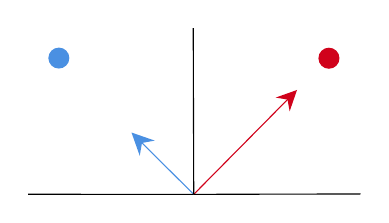
\begin{tikzpicture}[x=0.75pt,y=0.75pt,yscale=-1,xscale=1]
            %uncomment if require: \path (0,300); %set diagram left start at 0, and has height of 300
            
            %Straight Lines [id:da17586827840068286] 
            \draw [color={rgb, 255:red, 208; green, 2; blue, 27 }  ,draw opacity=1 ]   (190.24,200.32) -- (237.89,152.16) ;
            \draw [shift={(240,150.03)}, rotate = 494.69] [fill={rgb, 255:red, 208; green, 2; blue, 27 }  ,fill opacity=1 ][line width=0.08]  [draw opacity=0] (9.82,-4.72) -- (0,0) -- (9.82,4.72) -- (6.52,0) -- cycle    ;
            %Straight Lines [id:da23704064540856618] 
            \draw [color={rgb, 255:red, 74; green, 144; blue, 226 }  ,draw opacity=1 ]   (190.24,200.32) -- (162.38,172.64) ;
            \draw [shift={(160.25,170.53)}, rotate = 404.81] [fill={rgb, 255:red, 74; green, 144; blue, 226 }  ,fill opacity=1 ][line width=0.08]  [draw opacity=0] (10.72,-5.15) -- (0,0) -- (10.72,5.15) -- (7.12,0) -- cycle    ;
            %Shape: Circle [id:dp3839733612485111] 
            \draw  [color={rgb, 255:red, 208; green, 2; blue, 27 }  ,draw opacity=1 ][fill={rgb, 255:red, 208; green, 2; blue, 27 }  ,fill opacity=1 ] (250.58,134.73) .. controls (250.58,132.08) and (252.73,129.93) .. (255.38,129.93) .. controls (258.03,129.93) and (260.18,132.08) .. (260.18,134.73) .. controls (260.18,137.38) and (258.03,139.53) .. (255.38,139.53) .. controls (252.73,139.53) and (250.58,137.38) .. (250.58,134.73) -- cycle ;
            %Shape: Circle [id:dp009447430116501954] 
            \draw  [color={rgb, 255:red, 74; green, 144; blue, 226 }  ,draw opacity=1 ][fill={rgb, 255:red, 74; green, 144; blue, 226 }  ,fill opacity=1 ] (120.47,134.66) .. controls (120.47,132.02) and (122.61,129.88) .. (125.25,129.88) .. controls (127.89,129.88) and (130.03,132.02) .. (130.03,134.66) .. controls (130.03,137.29) and (127.89,139.43) .. (125.25,139.43) .. controls (122.61,139.43) and (120.47,137.29) .. (120.47,134.66) -- cycle ;
            %Straight Lines [id:da5714219654763008] 
            \draw    (190,120.28) -- (190.24,200.32) ;
            %Straight Lines [id:da22247567054966455] 
            \draw    (110.5,200.28) -- (190.24,200.32) ;
            %Straight Lines [id:da4124676757039665] 
            \draw    (270.64,200.12) -- (190.24,200.32) ;
            
            
            
            
            \end{tikzpicture}
    \end{adjustbox}
  \end{center}
\caption{\textbf{Motivation as a vector}. Blue and red dots represent two objects with different characteristics while the two arrows illustrate the hypothetical motivational propensity of an individual (or two individuals) towards them. The black segments delineate the space created by the combination of the objects' characteristics and the motivational propensity of the individuals. Here the red object has the potential to generate more behaviour than the blue object possibly as a result of its characteristics and those of the individual interacting with it.}
\label{fig: vect_mot}
\end{figure}
Summarizing we can say that from a motivational point of view, the behaviour of an individual is driven by the expectancy of pleasurable outcomes derived by the goal the behaviour is aiming to reach \cite{berridge2004motivation}. Therefore, if motivation acts as a single overarching process, we expect it to hold predictive and explanatory power over goal directed behaviour seamlessly across a heterogeneous range of situations and individuals. Motivational theories based on the concepts of reward and incentive are promising candidates for this because, relying on consistent and plausible psychobiological bases, they tend to operate abstracting from the nature of the individuals and the objects. \cite{ikemoto1999role,berridge1998role,salamone2002motivational,berridge2004motivation,armony2013cambridge,corbit2015learning}.

\subsection{An Historical View on Reward-driven Motivation}
\label{motivation_hist}
Introducing the processes of classical and operant conditioning is an essential step for describing theories of reward-driven motivation, in particular if we are interested in their behavioural correlates. Both constructs heavily rely on the general concepts of reinforcer and reinforcement process. Simply put, reinforcers are those objects or actions that have the ability to alter the likelyhood of appearance of specific behaviours \cite{kling1971woodworth,skinner1953science,squire2012fundamental}. A reinforcement process instead define the learning mechanisms by which a specific behaviour becomes, over time, more or less probable conditional on the presence of particular reinforcers \cite{kling1971woodworth}. In this view we can think of classical and operant conditioning as two complementary oprationalizations of the reinforcement process. Classical conditioning describes the learning process in which, independently from the activity of an individual, the repeated pairing of two objects will cause one to acquire the eliciting properties of the other \cite{squire2012fundamental}. In other words, the repeated pairing of a neutral object with reinforcing consequences will imbue the first with reinforcement properties making it a reinforcer. Operant conditioning on the other hand, extends the concept of classical conditioning introducing the agency of the individual \cite{skinner1953science}. The frequency of behaviour produced by an individual tends to increase when precise consequences are associated to it \cite{skinner1953science}. In this view, an operant is formalized as a goal directed behaviour while all the elements reinforcing the re-iteration of this behaviour are called reinforcers \cite{skinner1953science}. The learning process here results from the relationship between a behaviour and its consequences, therefore the probability of behaviour to take place is related to its capability to generate reinforcer \cite{kling1971woodworth}. Both classical and operant conditioning are of course very simplistic accounts of human behaviour, but nevertheless able to succinctly illustrate a fundamental process by which most (if not all) individuals are able to learn and leverage the association between actions and the positive (i.e. rewarding) consequences associated to them. In this regard, it is not surprising that many theories of reward-driven motivation stem directly from these two constructs. For example, in its work Bolles \cite{bolles1972reinforcement} suggested that individuals were motivated by the "expectations of incentive outcomes". These expectations are formed through a learning process where an association between actions and potential pleasurable outcomes is created \cite{bolles1972reinforcement,berridge2004motivation}. Expanding on this idea, Bindra suggested that the learning process does not just generate pleasure expectations in response to specific behaviours but it also allows individuals to perceive the behaviours themselves as a source of hedonic reward \cite{bindra1978adaptive,berridge2004motivation}.
This introduces the concept of learning through reinforcement: an object and the behaviours associated to it become relevant and salient for an individual as a consequence of learning its incentive properties \cite{berridge2004motivation}. A third theoretical formulation by Toates \cite{toates1994comparing}, asserted that the magnitude of the perceived incentives introduced by both Bolles and Bindra is modulated by the internal states of the individual \cite{toates1994comparing,berridge2004motivation}. In other words, the incentive expectations (and consequently the associated motivated behaviours) learned by an individual can change over time depending on the individual's internal state. Until now we have mainly used the terms reinforces and incentives for identifying objects able to drive and shape behaviour, but when it comes to define effective reinforces, it is not just a matter of merely pairing a behaviour with a stimulus but the stimulus itself has to have particular properties. In this view, stimuli able to generate pleasurable feelings in the individual are the best candidates for being effective reinforces, they are said having ‘rewarding properties’. But what is, and how can be defined the reward? The reward is a process generated in response to a stimulus making it desirable for its capacity to generate pleasurable responses. In this view, for being able to generate rewarding response, a stimulus needs two fundamental properties: it has to be wanted (i.e. it acquires the capacity to become desirable) and liked (i.e. it has to be able to generate pleasure in the individual) \cite{berridge2009dissecting}. But how a particular object acquires these properties? This is mostly carried out by the same learning processes mentioned in section \ref{motivation_hist}. The repeated pairing of a stimulus with the (positive) consequences it exerts on the individual will imbue the first with so called rewarding properties. Moreover, through operant conditioning  not just the stimulus itself but also the connected instrumental behaviour will likely acquire the same rewarding properties \cite{berridge2009dissecting}. As anticipated in section \ref{motivation}, a useful distinction that can be made is between objects having primary and secondary reward properties. Objects linked with essential evolutionary needs (i.e. satisfaction of homeostatic needs) are on a fast track for becoming reinforcers, their rewarding properties don’t have to be learned but are, up to a certain extent, intrinsic to them \cite{sescousse2013processing}. Classical examples of primary rewards are food, mating-related activities and drug of abuse \cite{berridge2004motivation, simpson2016behavioral}. On the other hand, objects with so called secondary rewarding properties don’t hold an innate capacity to generate pleasurable experiences, this capacity is acquired by means of the same learning mechanisms we've just presented \cite{sescousse2013processing}. 

\subsection{The Incentive Salience Theory of Motivation}
\label{incentive_salience}
The approaches proposed by Bolles, Bindra and Toates,  provide an account of reward-based motivation but they assume that there is no distinction between the affective dimension of an incentive (i.e. how pleasurable it is) and the purely motivational aspect of it (i.e. how much goal directed behaviour it can produce) \cite{bindra1978adaptive,toates1994comparing}. Expanding on this, Berridge and Robinson proposed that the motivational process controlling the interaction between individuals and objects might not be a unitary mechanism but rather a composite process having specific and dissociable components which rely on specialized neurobiological mechanisms, namely: \emph{liking}, \emph{wanting} and \emph{learning} \cite{berridge1998role,berridge2009dissecting,smith2011disentangling}.

\paragraph*{Liking}
\label{liking}
The \emph{liking} component describes the pleasure expected by an individual when interacting with an object \cite{berridge2009dissecting}. It is responsible for the hedonic quality of an experience and acts as a signal indicating that interacting again with that object might be beneficial. Despite the fact that \emph{liking} plays an important role in the incentive salience hypothesis of motivation it is difficult to measure it outside controlled laboratory environments \cite{berridge1998role} and it will not form a central theme of this thesis. Instead, we will focus on the "wanting" and "learning" components.

\paragraph*{Wanting}
\label{wanting}
The \emph{wanting} component, or "incentive salience", has the function of generating and holding latent representation of objects and behavioural acts and of attributing value to them through learning mechanisms. These "valued representations" can then be used by action selection systems in order to make certain behaviours more likely \cite{ikemoto1996dissociations,berridge1998role,mcclure2003computational,berridge2004motivation}. As a consequence of this, when an object is attributed with incentive salience it will more likely draw the subject's attention and become the focus of goal directed behaviours \cite{berridge2004motivation}. Interestingly, \emph{wanting} seems to be more than a simple form of value-caching but rather a dynamic process in constant change \cite{robinson1993neural,zhang2009neural,tindell2009dynamic,berridge2012prediction}. This is because the saliency of an object depends both on its attributed value but also on the state of the individual interacting with it. A change in the individual's internal state can dampen, magnify or even revert the amount of attributed salience. \cite{robinson1993neural,zhang2009neural,tindell2009dynamic,berridge2012prediction}. It is important to note that \emph{wanting} is not the hedonic expectation associated to an object, (which is designated by \emph{liking}), but rather the process promoting the approach towards an object and the interaction with it \cite{berridge2009dissecting,robinson2015roles}. Despite the fact that \emph{liking} and \emph{wanting} are often correlated (i.e. I want what I like and vice versa) they can occasionally be triggered separately: addictive behaviours for instance are a notable example of \emph{wanting} without \emph{liking} \cite{robinson1993neural}. The functional dissociation between these two components is linked to differences in the underlying neurobiological substrate \cite{berridge2009dissecting,smith2011disentangling}. Neurotransmitters and brain areas responsible for \emph{wanting} appear to be more numerous, diverse and easily activated than those for \emph{liking} \cite{berridge2009dissecting,robinson2015roles}. As a consequence, increased incentive salience can be obtained by raising dopamine levels in many portion of the striatum without the need for the synchronized activity in other areas \cite{berridge2009dissecting,smith2011disentangling,meyer2015motivational}. This implies that the \emph{wanting} component tends to produce more robust behavioural indicators in the form of increased amount and frequency of interactions between an individual and an object \cite{berridge1998role}, which makes it a promising candidate for behavioural studies in conditions where strict experimental control is not possible.

\paragraph*{Learning}
\label{learning}
The last component in the formulation proposed by Berridge and Robinson \cite{berridge1998role,berridge2004motivation} consists of mechanisms that provide an individual with the capability to predict, based on past experiences, the occurrence of future pleasurable outcomes (i.e. \emph{liking} reactions) when interacting with specific objects. These are similar to the learning processes illustrated in section \ref{motivation_hist} and have a twofold function. These mechanisms allow the attribution and change of incentive salience properties to previously \emph{liked} objects (e.g. primary reward objects) but they also enable subjects to learn the hedonic value of initially neutral stimuli (e.g. secondary reward objects). The \emph{learning} mechanism is based on classical conditioning: through repeated interactions with an object an individual will learn its hedonic properties and consequently attribute incentive salience to it \cite{berridge2004motivation,berridge2009dissecting}. This process is driven by mechanisms similar to those of reward-prediction error: learning is driven by spikes in dopaminergic activity generated by a mismatch between expected and experienced rewards. \cite{schultz1997neural,schultz2000multiple,flagel2011selective}.

\section{Engagement as a Derivative of Motivation}
\label{engagement}
We will now momentarily diverge from our discussion on motivation for introducing the construct of engagement. The reason for this brief detour lies in the fact that presenting the construct of engagement allows us to better understand the practical implication that motivational processes have in our everyday life. Despite engagement has applications in a wide range of contexts, we think it is better understood when framed within a specific class of activities. In this view, given the background from which this work has arisen, we will focus on the area of videogames but we will make evident how, by framing engagement as a byproduct of motivational processes, we can easily generalize it to other type of activities.

\subsection{Theories of Engagement}
\label{factors_engagement}
Playing games has always been present in human history as an occupation aiming to entertain and relax \cite{connolly2012systematic}, it can be defined as a free-time activity with spatial and temporal boundaries able to intensely absorb who is involved in it \cite{connolly2012systematic}. A special case of the broader group of games are those delivered and experienced in a digital format (i.e. videogames) which in the last decades has been substituting more traditional playful activities \cite{boyle2012engagement,connolly2012systematic}. This phenomenon has been reflected both in terms of number of people involved in playing videogames as well as in the amount of time spent engaging in this activity \cite{boyle2012engagement}. One of the main reasons for this explosive phenomenon is the fact that videogames seems to be perfect medium for delivering pleasurable experiences \cite{boyle2012engagement}, consequently holding a strong potential to engage and retain users involved in the playing activity. Various attempt has been made to understand engagement in videogames, both as unitary process and at the level of factors driving and influencing it \cite{boyle2012engagement}. The literature on the subject is abundant although extremely heterogeneous \cite{boyle2012engagement}. A clear example of this heterogeneity is the definition of engagement provided by O'Brien et al. \cite{o2008user}:
\\
\\
\textit{"...a quality of user experiences with technology that is characterized by challenge, aesthetic and sensory appeal, feedback, novelty, interactivity, perceived control and time, awareness, motivation, interest and affect..."}
\\
\\
this definition, although providing a good holistic description, makes it exceptionally hard to clearly define a unitary framework for defining engagement let alone specifying its mechanistic aspects. This lack of theoretical formalism is reflected in most (if not all) accounts of engagement and, to a certain extent, inevitable given the breadth of the behavioural, cognitive and affective aspects that the construct tries to cover. Nevertheless, inspecting some of the most prominent theories of engagement we can individuate some common themes useful for composing a unifed framework.

\paragraph*{Flow} This is a classical construct often occurring in the videogame literature for explaining the phenomenon of engagement. Developed by Csikszentmihalyi \cite{csikszentmihalyi2014toward}, the construct of flow prescribes that when an individual is absorbed in an activity perceived as valuable they will experience a rewarding state of optimal pleasure constituting the fuel for of engagement process \cite{boyle2012engagement}. In this view, conditio sine qua non for the flow state to arise is a balanced combination of the individual’ state level and the characteristics of the interaction in which they are involved \cite{boyle2012engagement,csikszentmihalyi2014toward}. Despite offering an interesting point of view, the concept of flow as a framework for explaining engagement might be prone to the fallacy of circular reasoning: is an individual engaged in a specific activity because this provides the optimal flow experience or this last one is a bi-product of being engaged in the activity itself? 

\paragraph*{Immersion} This construct is closely connected to that of flow but specifically concerned with the psychological experience of engaging with a computer game \cite{jennett2008measuring}. Immersion tries to describe the experience of engaging in a specific moment in time with a videogame  rather than posing itself as a factor influencing or driving engagement \cite{jennett2008measuring}. According to Jennet et al. \cite{jennett2008measuring}, as a result of a good gaming experience, an individual might loose track of time and space and will experience a sense of being completely "immersed" in the playing activity.

\paragraph*{Uses and gratification} This theory states that the consumption of media is a way for individuals to satisfy the need for gratification (i.e. reward). The gratification-seeking behaviour is then driven and characterized by the nature of the underlying motive generating them (e.g. my need to connect with other people drives my social-media consumption) \cite{lucas2004sex}. Again, according to this theory, individuals are not passive bystanders but will actively interact with a specific media object based on its ability to meet the individual's underlying motivational drive. Uses and gratification theory introduce two important concepts: first that individuals engage in a spontaneous activity (i.e. media object interaction) in search of some form of gratification and second that this interaction is not passive but rather an active process.

\subsubsection{The Engagement Process Model}
\label{eng_proc_model}
We will focus now on an relatively atypical formalization of the construct of engagement, the engagement process model formulated by O'Brien and colleagues \cite{o2008user}. This framework, instead of presenting engagement as a static entity proposes the idea that it is better understood as a dynamic process \cite{o2008user}. O'Brien et al. avoid to give an exact definition of engagement but rather describe it as a process with distinct phases each one possessing peculiar attributes \cite{o2008user}:
\begin{figure}[h]
\begin{center}
\begin{adjustbox}{width=\textwidth}

\tikzset {_ja3qzis2s/.code = {\pgfsetadditionalshadetransform{ \pgftransformshift{\pgfpoint{0 bp } { 0 bp }  }  \pgftransformrotate{0 }  \pgftransformscale{2 }  }}}
\pgfdeclarehorizontalshading{_2clqcmsm1}{150bp}{rgb(0bp)=(0.88,0.88,0.88);
rgb(37.5bp)=(0.88,0.88,0.88);
rgb(49.53571319580078bp)=(0.88,0.88,0.88);
rgb(62.5bp)=(1,0,0);
rgb(100bp)=(1,0,0)}
\tikzset{_wutnxytpv/.code = {\pgfsetadditionalshadetransform{\pgftransformshift{\pgfpoint{0 bp } { 0 bp }  }  \pgftransformrotate{0 }  \pgftransformscale{2 } }}}
\pgfdeclarehorizontalshading{_i9ez78zk2} {150bp} {color(0bp)=(transparent!61);
color(37.5bp)=(transparent!61);
color(49.53571319580078bp)=(transparent!75);
color(62.5bp)=(transparent!75);
color(100bp)=(transparent!75) } 
\pgfdeclarefading{_v08dyi49j}{\tikz \fill[shading=_i9ez78zk2,_wutnxytpv] (0,0) rectangle (50bp,50bp); } 

% Gradient Info
  
\tikzset {_v10pg96dp/.code = {\pgfsetadditionalshadetransform{ \pgftransformshift{\pgfpoint{0 bp } { 0 bp }  }  \pgftransformrotate{0 }  \pgftransformscale{2 }  }}}
\pgfdeclarehorizontalshading{_z95a3b8ok}{150bp}{rgb(0bp)=(1,0,0);
rgb(37.5bp)=(1,0,0);
rgb(62.5bp)=(0,0,1);
rgb(100bp)=(0,0,1)}
\tikzset{_f3vm7u4s3/.code = {\pgfsetadditionalshadetransform{\pgftransformshift{\pgfpoint{0 bp } { 0 bp }  }  \pgftransformrotate{0 }  \pgftransformscale{2 } }}}
\pgfdeclarehorizontalshading{_s7qnsrg0u} {150bp} {color(0bp)=(transparent!75);
color(37.5bp)=(transparent!75);
color(62.5bp)=(transparent!75);
color(100bp)=(transparent!75) } 
\pgfdeclarefading{_iduaxypal}{\tikz \fill[shading=_s7qnsrg0u,_f3vm7u4s3] (0,0) rectangle (50bp,50bp); } 

% Gradient Info
  
\tikzset {_q92g98s98/.code = {\pgfsetadditionalshadetransform{ \pgftransformshift{\pgfpoint{0 bp } { 0 bp }  }  \pgftransformrotate{0 }  \pgftransformscale{2 }  }}}
\pgfdeclarehorizontalshading{_0mqi486xx}{150bp}{rgb(0bp)=(0,0,1);
rgb(37.5bp)=(0,0,1);
rgb(62.5bp)=(0,0,1);
rgb(100bp)=(0,0,1)}
\tikzset{_hpxpij7iw/.code = {\pgfsetadditionalshadetransform{\pgftransformshift{\pgfpoint{0 bp } { 0 bp }  }  \pgftransformrotate{0 }  \pgftransformscale{2 } }}}
\pgfdeclarehorizontalshading{_5uin3k9a8} {150bp} {color(0bp)=(transparent!75);
color(37.5bp)=(transparent!75);
color(62.5bp)=(transparent!50);
color(100bp)=(transparent!50) } 
\pgfdeclarefading{_lm1jjwudb}{\tikz \fill[shading=_5uin3k9a8,_hpxpij7iw] (0,0) rectangle (50bp,50bp); } 

% Gradient Info
  
\tikzset {_31yctqmge/.code = {\pgfsetadditionalshadetransform{ \pgftransformshift{\pgfpoint{0 bp } { 0 bp }  }  \pgftransformrotate{0 }  \pgftransformscale{2 }  }}}
\pgfdeclarehorizontalshading{_3ntqju468}{150bp}{rgb(0bp)=(1,0,0);
rgb(37.5bp)=(1,0,0);
rgb(62.5bp)=(0.03,0,1);
rgb(100bp)=(0.03,0,1)}
\tikzset{_xkldkwpsn/.code = {\pgfsetadditionalshadetransform{\pgftransformshift{\pgfpoint{0 bp } { 0 bp }  }  \pgftransformrotate{0 }  \pgftransformscale{2 } }}}
\pgfdeclarehorizontalshading{_idcgzsidk} {150bp} {color(0bp)=(transparent!75);
color(37.5bp)=(transparent!75);
color(62.5bp)=(transparent!75);
color(100bp)=(transparent!75) } 
\pgfdeclarefading{_4908ehgtf}{\tikz \fill[shading=_idcgzsidk,_xkldkwpsn] (0,0) rectangle (50bp,50bp); } 
\tikzset{every picture/.style={line width=0.75pt}} %set default line width to 0.75pt        

\begin{tikzpicture}[x=0.75pt,y=0.75pt,yscale=-1,xscale=1]
%uncomment if require: \path (0,160); %set diagram left start at 0, and has height of 160

%Rounded Rect [id:dp8177682455870696] 
\path  [shading=_2clqcmsm1,_ja3qzis2s,path fading= _v08dyi49j ,fading transform={xshift=2}] (40.4,39.66) .. controls (40.4,35.17) and (44.04,31.52) .. (48.53,31.52) -- (131.24,31.52) .. controls (135.73,31.52) and (139.37,35.17) .. (139.37,39.66) -- (139.37,64.06) .. controls (139.37,68.55) and (135.73,72.19) .. (131.24,72.19) -- (48.53,72.19) .. controls (44.04,72.19) and (40.4,68.55) .. (40.4,64.06) -- cycle ; % for fading 
 \draw   (40.4,39.66) .. controls (40.4,35.17) and (44.04,31.52) .. (48.53,31.52) -- (131.24,31.52) .. controls (135.73,31.52) and (139.37,35.17) .. (139.37,39.66) -- (139.37,64.06) .. controls (139.37,68.55) and (135.73,72.19) .. (131.24,72.19) -- (48.53,72.19) .. controls (44.04,72.19) and (40.4,68.55) .. (40.4,64.06) -- cycle ; % for border 

%Straight Lines [id:da7662528874093815] 
\draw    (139.6,52.56) -- (175.16,52.56) ;
\draw [shift={(178.16,52.56)}, rotate = 180] [fill={rgb, 255:red, 0; green, 0; blue, 0 }  ][line width=0.08]  [draw opacity=0] (10.72,-5.15) -- (0,0) -- (10.72,5.15) -- (7.12,0) -- cycle    ;
%Rounded Rect [id:dp7926455800001433] 
\path  [shading=_z95a3b8ok,_v10pg96dp,path fading= _iduaxypal ,fading transform={xshift=2}] (179.51,39.56) .. controls (179.51,35.07) and (183.16,31.43) .. (187.65,31.43) -- (271.95,31.43) .. controls (276.44,31.43) and (280.09,35.07) .. (280.09,39.56) -- (280.09,63.96) .. controls (280.09,68.45) and (276.44,72.1) .. (271.95,72.1) -- (187.65,72.1) .. controls (183.16,72.1) and (179.51,68.45) .. (179.51,63.96) -- cycle ; % for fading 
 \draw   (179.51,39.56) .. controls (179.51,35.07) and (183.16,31.43) .. (187.65,31.43) -- (271.95,31.43) .. controls (276.44,31.43) and (280.09,35.07) .. (280.09,39.56) -- (280.09,63.96) .. controls (280.09,68.45) and (276.44,72.1) .. (271.95,72.1) -- (187.65,72.1) .. controls (183.16,72.1) and (179.51,68.45) .. (179.51,63.96) -- cycle ; % for border 

%Straight Lines [id:da9273537542158072] 
\draw    (280.09,52.4) -- (315.09,52.4) ;
\draw [shift={(318.09,52.4)}, rotate = 180] [fill={rgb, 255:red, 0; green, 0; blue, 0 }  ][line width=0.08]  [draw opacity=0] (10.72,-5.15) -- (0,0) -- (10.72,5.15) -- (7.12,0) -- cycle    ;
%Rounded Rect [id:dp5551618546481307] 
\path  [shading=_0mqi486xx,_q92g98s98,path fading= _lm1jjwudb ,fading transform={xshift=2}] (320.37,40.79) .. controls (320.37,36.43) and (323.91,32.89) .. (328.28,32.89) -- (412.18,32.89) .. controls (416.55,32.89) and (420.09,36.43) .. (420.09,40.79) -- (420.09,64.51) .. controls (420.09,68.88) and (416.55,72.41) .. (412.18,72.41) -- (328.28,72.41) .. controls (323.91,72.41) and (320.37,68.88) .. (320.37,64.51) -- cycle ; % for fading 
 \draw   (320.37,40.79) .. controls (320.37,36.43) and (323.91,32.89) .. (328.28,32.89) -- (412.18,32.89) .. controls (416.55,32.89) and (420.09,36.43) .. (420.09,40.79) -- (420.09,64.51) .. controls (420.09,68.88) and (416.55,72.41) .. (412.18,72.41) -- (328.28,72.41) .. controls (323.91,72.41) and (320.37,68.88) .. (320.37,64.51) -- cycle ; % for border 

%Rounded Rect [id:dp4578454458037269] 
\path  [shading=_3ntqju468,_31yctqmge,path fading= _4908ehgtf ,fading transform={xshift=2}] (249.51,99.66) .. controls (249.51,95.2) and (253.13,91.59) .. (257.58,91.59) -- (341.73,91.59) .. controls (346.19,91.59) and (349.8,95.2) .. (349.8,99.66) -- (349.8,123.85) .. controls (349.8,128.31) and (346.19,131.92) .. (341.73,131.92) -- (257.58,131.92) .. controls (253.13,131.92) and (249.51,128.31) .. (249.51,123.85) -- cycle ; % for fading 
 \draw  [dash pattern={on 4.5pt off 4.5pt}] (249.51,99.66) .. controls (249.51,95.2) and (253.13,91.59) .. (257.58,91.59) -- (341.73,91.59) .. controls (346.19,91.59) and (349.8,95.2) .. (349.8,99.66) -- (349.8,123.85) .. controls (349.8,128.31) and (346.19,131.92) .. (341.73,131.92) -- (257.58,131.92) .. controls (253.13,131.92) and (249.51,128.31) .. (249.51,123.85) -- cycle ; % for border 

%Straight Lines [id:da8026549590400252] 
\draw    (419.92,52.56) -- (455.72,52.56) ;
\draw [shift={(458.72,52.56)}, rotate = 180] [fill={rgb, 255:red, 0; green, 0; blue, 0 }  ][line width=0.08]  [draw opacity=0] (10.72,-5.15) -- (0,0) -- (10.72,5.15) -- (7.12,0) -- cycle    ;
%Rounded Rect [id:dp9517655993514624] 
\draw  [fill={rgb, 255:red, 8; green, 0; blue, 255 }  ,fill opacity=0.5 ] (460.37,40.43) .. controls (460.37,35.98) and (463.98,32.37) .. (468.44,32.37) -- (552.59,32.37) .. controls (557.05,32.37) and (560.66,35.98) .. (560.66,40.43) -- (560.66,64.63) .. controls (560.66,69.09) and (557.05,72.7) .. (552.59,72.7) -- (468.44,72.7) .. controls (463.98,72.7) and (460.37,69.09) .. (460.37,64.63) -- cycle ;
%Curve Lines [id:da08756710454619077] 
\draw    (230.57,77.7) .. controls (230.32,112.22) and (230.67,111.83) .. (249.51,111.83) ;
\draw [shift={(230.6,74.4)}, rotate = 90.44] [fill={rgb, 255:red, 0; green, 0; blue, 0 }  ][line width=0.08]  [draw opacity=0] (10.72,-5.15) -- (0,0) -- (10.72,5.15) -- (7.12,0) -- cycle    ;
%Curve Lines [id:da642505597469857] 
\draw    (370.14,74.57) .. controls (369.57,112.29) and (370.09,112.11) .. (349.8,112.11) ;

% Text Node
\draw (89.09,50.86) node  [font=\fontsize{0.67em}{0.8em}\selectfont] [align=left] {\begin{minipage}[lt]{47.87pt}\setlength\topsep{0pt}
\begin{center}
{\large Point of}\\{\large Engagement}
\end{center}

\end{minipage}};
% Text Node
\draw (230.5,51.76) node  [font=\fontsize{0.67em}{0.8em}\selectfont] [align=left] {\begin{minipage}[lt]{47.87pt}\setlength\topsep{0pt}
\begin{center}
{\large Sustained}\\{\large Engagement}
\end{center}

\end{minipage}};
% Text Node
\draw (370.23,52.65) node  [font=\fontsize{0.67em}{0.8em}\selectfont] [align=left] {\begin{minipage}[lt]{47.87pt}\setlength\topsep{0pt}
\begin{center}
{\large Dis}\\{\large Engagement}
\end{center}

\end{minipage}};
% Text Node
\draw (510.51,52.53) node  [font=\fontsize{0.67em}{0.8em}\selectfont] [align=left] {\begin{minipage}[lt]{32.64pt}\setlength\topsep{0pt}
\begin{center}
{\large Extintion}
\end{center}

\end{minipage}};
% Text Node
\draw (300.67,111.76) node  [font=\fontsize{0.67em}{0.8em}\selectfont] [align=left] {\begin{minipage}[lt]{47.87pt}\setlength\topsep{0pt}
\begin{center}
{\large Re}\\{\large Engagement}
\end{center}

\end{minipage}};
% Text Node
\draw (29.33,14.97) node [anchor=north west][inner sep=0.75pt]   [align=left] {{\large 1}};
% Text Node
\draw (166.53,14.97) node [anchor=north west][inner sep=0.75pt]   [align=left] {{\large 2}};
% Text Node
\draw (308.2,14.3) node [anchor=north west][inner sep=0.75pt]   [align=left] {{\large 3}};
% Text Node
\draw (236.53,127.97) node [anchor=north west][inner sep=0.75pt]   [align=left] {{\large 4}};
% Text Node
\draw (446.73,14.3) node [anchor=north west][inner sep=0.75pt]   [align=left] {{\large 5}};
\end{tikzpicture}
\end{adjustbox}
\end{center}
\caption{\textbf{Diagram summarizing the different stages of the negagement process mode}.}
\label{fig: eng_proc_model_1}
\end{figure}
\paragraph*{Point of engagement} This is the starting point of the engagement process, it is the moment in which the individual’s attention is directed towards a specific object or activity due its properties and capacity to fulfil specific motivational drives.

\paragraph*{Period of engagement} This is the period during which the individual has a sustained interaction with the object of interest. In this case, a situation of sustained and prolonged interaction is conditional on the ability of the object to provide a positive and stimulating experience.

\paragraph*{Disengagement} This stage defines the moment in which the individual reduces the interaction with the object due to internal or external factors. The internal factors are usually connected to loss of interest or pressure derived by the time passing, external factors instead relate more to the inability of the activity to provide a positive experience or to the occurrence of external events in the environment surrounding the individual.

\paragraph*{Re-engagement} It identifies the moment in which the user returns to a sustained level of activity after disengagement occurred. This can happen both in the short and long term and it is the result of positive experiences with the activity, which are usually linked to be exposed to rewarding incentives or novel content within the activity.

\paragraph*{Extinction} In case of prolonged disengagement, marked unsatisfying experiences or impactful external events, the individual might terminate its interactions with the object leaving no further possibility to re-engage with it.

\subsection{From Motivation to Engagement}
\label{eng_reward_motivation}
What emerged from this brief overview of the literature is that engagement seems to be best described as a process controlled by the characteristics of an object, the internal state of the individual interacting with it and eventual environmental factors external to both. In this view engagement appears as a second order factor generated by the internal state of the individual and concerned with the description and quantification  of their interactions with an object  \cite{lucas2004sex,o2008user,jennett2008measuring,boyle2012engagement,connolly2012systematic,csikszentmihalyi2014toward}.The quality and quantity of these interactions seem to be conditional on the ability of the object to provide feelings of enjoyment and pleasure \cite{lucas2004sex,o2008user,jennett2008measuring,boyle2012engagement,connolly2012systematic,csikszentmihalyi2014toward}. We can already see a connection between the construct of engagement and the reward-driven motivational processes presented in section \ref{motivation}, especially if we look at the behavioural level. In the context of videogames, motivational processes seem to pertain the formation and modulation of unobservable (i.e. latent) states characterizing the individual before, during and after the interaction with a videogame. On the other hand, engagement appears to describe the observable aspects of this interaction both at the behavioural and experiential level \cite{lucas2004sex,o2008user,jennett2008measuring,boyle2012engagement,connolly2012systematic,csikszentmihalyi2014toward}. A more clear illustration of this idea is presented in Figure \ref{fig: eng_proc_model_2} 
\begin{figure}[h]
\begin{center}
\begin{adjustbox}{width=\columnwidth}

\tikzset {_tol09vz9c/.code = {\pgfsetadditionalshadetransform{ \pgftransformshift{\pgfpoint{0 bp } { 0 bp }  }  \pgftransformrotate{0 }  \pgftransformscale{2 }  }}}
\pgfdeclarehorizontalshading{_j7rsmr3nr}{150bp}{rgb(0bp)=(0.93,0.93,0.93);
rgb(37.5bp)=(0.93,0.93,0.93);
rgb(62.5bp)=(1,0,0);
rgb(100bp)=(1,0,0)}
\tikzset{_yxq6cdpsj/.code = {\pgfsetadditionalshadetransform{\pgftransformshift{\pgfpoint{0 bp } { 0 bp }  }  \pgftransformrotate{0 }  \pgftransformscale{2 } }}}
\pgfdeclarehorizontalshading{_7yg524gtp} {150bp} {color(0bp)=(transparent!75);
color(37.5bp)=(transparent!75);
color(62.5bp)=(transparent!75);
color(100bp)=(transparent!75) } 
\pgfdeclarefading{_y4z1b8bbb}{\tikz \fill[shading=_7yg524gtp,_yxq6cdpsj] (0,0) rectangle (50bp,50bp); } 

% Gradient Info
  
\tikzset {_3ywdqyfah/.code = {\pgfsetadditionalshadetransform{ \pgftransformshift{\pgfpoint{0 bp } { 0 bp }  }  \pgftransformrotate{0 }  \pgftransformscale{2 }  }}}
\pgfdeclarehorizontalshading{_2t0kw1fpw}{150bp}{rgb(0bp)=(1,0,0);
rgb(37.5bp)=(1,0,0);
rgb(62.5bp)=(0,0,1);
rgb(100bp)=(0,0,1)}
\tikzset{_yvsljnreh/.code = {\pgfsetadditionalshadetransform{\pgftransformshift{\pgfpoint{0 bp } { 0 bp }  }  \pgftransformrotate{0 }  \pgftransformscale{2 } }}}
\pgfdeclarehorizontalshading{_fpvhgjdei} {150bp} {color(0bp)=(transparent!75);
color(37.5bp)=(transparent!75);
color(62.5bp)=(transparent!75);
color(100bp)=(transparent!75) } 
\pgfdeclarefading{_y32y00acn}{\tikz \fill[shading=_fpvhgjdei,_yvsljnreh] (0,0) rectangle (50bp,50bp); } 

% Gradient Info
  
\tikzset {_k82gbaai2/.code = {\pgfsetadditionalshadetransform{ \pgftransformshift{\pgfpoint{0 bp } { 0 bp }  }  \pgftransformrotate{0 }  \pgftransformscale{2 }  }}}
\pgfdeclarehorizontalshading{_mzd6axxaa}{150bp}{rgb(0bp)=(0,0,1);
rgb(37.5bp)=(0,0,1);
rgb(62.5bp)=(0,0,1);
rgb(100bp)=(0,0,1)}
\tikzset{_1ih9fwhej/.code = {\pgfsetadditionalshadetransform{\pgftransformshift{\pgfpoint{0 bp } { 0 bp }  }  \pgftransformrotate{0 }  \pgftransformscale{2 } }}}
\pgfdeclarehorizontalshading{_py52u7ab2} {150bp} {color(0bp)=(transparent!75);
color(37.5bp)=(transparent!75);
color(62.5bp)=(transparent!50);
color(100bp)=(transparent!50) } 
\pgfdeclarefading{_wr0vkxl3y}{\tikz \fill[shading=_py52u7ab2,_1ih9fwhej] (0,0) rectangle (50bp,50bp); } 

% Gradient Info
  
\tikzset {_3kvg59946/.code = {\pgfsetadditionalshadetransform{ \pgftransformshift{\pgfpoint{0 bp } { 0 bp }  }  \pgftransformrotate{-90 }  \pgftransformscale{2 }  }}}
\pgfdeclarehorizontalshading{_wvh4fdo7p}{150bp}{rgb(0bp)=(1,0,0);
rgb(37.5bp)=(1,0,0);
rgb(62.5bp)=(0,0,1);
rgb(100bp)=(0,0,1)}
\tikzset{_dv8t3n3dv/.code = {\pgfsetadditionalshadetransform{\pgftransformshift{\pgfpoint{0 bp } { 0 bp }  }  \pgftransformrotate{-90 }  \pgftransformscale{2 } }}}
\pgfdeclarehorizontalshading{_abfcxja44} {150bp} {color(0bp)=(transparent!75);
color(37.5bp)=(transparent!75);
color(62.5bp)=(transparent!75);
color(100bp)=(transparent!75) } 
\pgfdeclarefading{_tndnn1d2b}{\tikz \fill[shading=_abfcxja44,_dv8t3n3dv] (0,0) rectangle (50bp,50bp); } 

% Gradient Info
  
\tikzset {_475pso13i/.code = {\pgfsetadditionalshadetransform{ \pgftransformshift{\pgfpoint{0 bp } { 0 bp }  }  \pgftransformrotate{-90 }  \pgftransformscale{2 }  }}}
\pgfdeclarehorizontalshading{_f5gjc5tzr}{150bp}{rgb(0bp)=(0,0,1);
rgb(37.5bp)=(0,0,1);
rgb(62.5bp)=(1,0,0);
rgb(100bp)=(1,0,0)}
\tikzset{_fwuteqqte/.code = {\pgfsetadditionalshadetransform{\pgftransformshift{\pgfpoint{0 bp } { 0 bp }  }  \pgftransformrotate{-90 }  \pgftransformscale{2 } }}}
\pgfdeclarehorizontalshading{_gbjam9yyh} {150bp} {color(0bp)=(transparent!75);
color(37.5bp)=(transparent!75);
color(62.5bp)=(transparent!75);
color(100bp)=(transparent!75) } 
\pgfdeclarefading{_wo5obn5gu}{\tikz \fill[shading=_gbjam9yyh,_fwuteqqte] (0,0) rectangle (50bp,50bp); } 
\tikzset{every picture/.style={line width=0.75pt}} %set default line width to 0.75pt        

\begin{tikzpicture}[x=0.75pt,y=0.75pt,yscale=-1,xscale=1]
%uncomment if require: \path (0,357); %set diagram left start at 0, and has height of 357

%Rounded Rect [id:dp08887598870261693] 
\draw  [fill={rgb, 255:red, 236; green, 236; blue, 236 }  ,fill opacity=1 ] (30.4,81.08) .. controls (30.4,76.59) and (34.04,72.95) .. (38.53,72.95) -- (121.24,72.95) .. controls (125.73,72.95) and (129.37,76.59) .. (129.37,81.08) -- (129.37,105.48) .. controls (129.37,109.97) and (125.73,113.61) .. (121.24,113.61) -- (38.53,113.61) .. controls (34.04,113.61) and (30.4,109.97) .. (30.4,105.48) -- cycle ;
%Rounded Rect [id:dp06222122397376195] 
\draw  [fill={rgb, 255:red, 236; green, 236; blue, 236 }  ,fill opacity=1 ] (200.51,81.08) .. controls (200.51,76.59) and (204.16,72.95) .. (208.65,72.95) -- (292.95,72.95) .. controls (297.44,72.95) and (301.09,76.59) .. (301.09,81.08) -- (301.09,105.48) .. controls (301.09,109.97) and (297.44,113.61) .. (292.95,113.61) -- (208.65,113.61) .. controls (204.16,113.61) and (200.51,109.97) .. (200.51,105.48) -- cycle ;
%Rounded Rect [id:dp7821816318063516] 
\draw  [fill={rgb, 255:red, 236; green, 236; blue, 236 }  ,fill opacity=1 ] (368.77,81.42) .. controls (368.77,77.06) and (372.31,73.52) .. (376.68,73.52) -- (460.58,73.52) .. controls (464.95,73.52) and (468.49,77.06) .. (468.49,81.42) -- (468.49,105.14) .. controls (468.49,109.5) and (464.95,113.04) .. (460.58,113.04) -- (376.68,113.04) .. controls (372.31,113.04) and (368.77,109.5) .. (368.77,105.14) -- cycle ;
%Rounded Rect [id:dp20372970008362923] 
\draw  [fill={rgb, 255:red, 236; green, 236; blue, 236 }  ,fill opacity=1 ] (535.37,81.18) .. controls (535.37,76.73) and (538.98,73.12) .. (543.44,73.12) -- (627.59,73.12) .. controls (632.05,73.12) and (635.66,76.73) .. (635.66,81.18) -- (635.66,105.38) .. controls (635.66,109.83) and (632.05,113.44) .. (627.59,113.44) -- (543.44,113.44) .. controls (538.98,113.44) and (535.37,109.83) .. (535.37,105.38) -- cycle ;
%Shape: Circle [id:dp19552380180112794] 
\path  [shading=_j7rsmr3nr,_tol09vz9c,path fading= _y4z1b8bbb ,fading transform={xshift=2}] (146.05,93.28) .. controls (146.05,84) and (153.57,76.48) .. (162.85,76.48) .. controls (172.13,76.48) and (179.65,84) .. (179.65,93.28) .. controls (179.65,102.56) and (172.13,110.08) .. (162.85,110.08) .. controls (153.57,110.08) and (146.05,102.56) .. (146.05,93.28) -- cycle ; % for fading 
 \draw  [dash pattern={on 4.5pt off 4.5pt}] (146.05,93.28) .. controls (146.05,84) and (153.57,76.48) .. (162.85,76.48) .. controls (172.13,76.48) and (179.65,84) .. (179.65,93.28) .. controls (179.65,102.56) and (172.13,110.08) .. (162.85,110.08) .. controls (153.57,110.08) and (146.05,102.56) .. (146.05,93.28) -- cycle ; % for border 

%Shape: Circle [id:dp27430889542654724] 
\path  [shading=_2t0kw1fpw,_3ywdqyfah,path fading= _y32y00acn ,fading transform={xshift=2}] (317.46,93.28) .. controls (317.46,84) and (324.98,76.48) .. (334.26,76.48) .. controls (343.54,76.48) and (351.06,84) .. (351.06,93.28) .. controls (351.06,102.56) and (343.54,110.08) .. (334.26,110.08) .. controls (324.98,110.08) and (317.46,102.56) .. (317.46,93.28) -- cycle ; % for fading 
 \draw  [dash pattern={on 4.5pt off 4.5pt}] (317.46,93.28) .. controls (317.46,84) and (324.98,76.48) .. (334.26,76.48) .. controls (343.54,76.48) and (351.06,84) .. (351.06,93.28) .. controls (351.06,102.56) and (343.54,110.08) .. (334.26,110.08) .. controls (324.98,110.08) and (317.46,102.56) .. (317.46,93.28) -- cycle ; % for border 

%Rounded Rect [id:dp4578454458037269] 
\draw  [fill={rgb, 255:red, 236; green, 236; blue, 236 }  ,fill opacity=1 ] (284.11,148.66) .. controls (284.11,144.2) and (287.73,140.59) .. (292.18,140.59) -- (376.33,140.59) .. controls (380.79,140.59) and (384.4,144.2) .. (384.4,148.66) -- (384.4,172.85) .. controls (384.4,177.31) and (380.79,180.92) .. (376.33,180.92) -- (292.18,180.92) .. controls (287.73,180.92) and (284.11,177.31) .. (284.11,172.85) -- cycle ;
%Shape: Circle [id:dp8141702965644008] 
\path  [shading=_mzd6axxaa,_k82gbaai2,path fading= _wr0vkxl3y ,fading transform={xshift=2}] (484.05,93.28) .. controls (484.05,84) and (491.57,76.48) .. (500.85,76.48) .. controls (510.13,76.48) and (517.65,84) .. (517.65,93.28) .. controls (517.65,102.56) and (510.13,110.08) .. (500.85,110.08) .. controls (491.57,110.08) and (484.05,102.56) .. (484.05,93.28) -- cycle ; % for fading 
 \draw  [dash pattern={on 4.5pt off 4.5pt}] (484.05,93.28) .. controls (484.05,84) and (491.57,76.48) .. (500.85,76.48) .. controls (510.13,76.48) and (517.65,84) .. (517.65,93.28) .. controls (517.65,102.56) and (510.13,110.08) .. (500.85,110.08) .. controls (491.57,110.08) and (484.05,102.56) .. (484.05,93.28) -- cycle ; % for border 

%Shape: Circle [id:dp5389996328417695] 
\path  [shading=_wvh4fdo7p,_3kvg59946,path fading= _tndnn1d2b ,fading transform={xshift=2}] (234.05,160.76) .. controls (234.05,151.48) and (241.57,143.96) .. (250.85,143.96) .. controls (260.13,143.96) and (267.65,151.48) .. (267.65,160.76) .. controls (267.65,170.03) and (260.13,177.56) .. (250.85,177.56) .. controls (241.57,177.56) and (234.05,170.03) .. (234.05,160.76) -- cycle ; % for fading 
 \draw  [dash pattern={on 4.5pt off 4.5pt}] (234.05,160.76) .. controls (234.05,151.48) and (241.57,143.96) .. (250.85,143.96) .. controls (260.13,143.96) and (267.65,151.48) .. (267.65,160.76) .. controls (267.65,170.03) and (260.13,177.56) .. (250.85,177.56) .. controls (241.57,177.56) and (234.05,170.03) .. (234.05,160.76) -- cycle ; % for border 

%Shape: Circle [id:dp655926787503073] 
\path  [shading=_f5gjc5tzr,_475pso13i,path fading= _wo5obn5gu ,fading transform={xshift=2}] (403.43,160.76) .. controls (403.43,151.48) and (410.95,143.96) .. (420.23,143.96) .. controls (429.51,143.96) and (437.03,151.48) .. (437.03,160.76) .. controls (437.03,170.03) and (429.51,177.56) .. (420.23,177.56) .. controls (410.95,177.56) and (403.43,170.03) .. (403.43,160.76) -- cycle ; % for fading 
 \draw  [dash pattern={on 4.5pt off 4.5pt}] (403.43,160.76) .. controls (403.43,151.48) and (410.95,143.96) .. (420.23,143.96) .. controls (429.51,143.96) and (437.03,151.48) .. (437.03,160.76) .. controls (437.03,170.03) and (429.51,177.56) .. (420.23,177.56) .. controls (410.95,177.56) and (403.43,170.03) .. (403.43,160.76) -- cycle ; % for border 

%Shape: Rectangle [id:dp8053989914309859] 
\draw   (9.1,51.6) -- (659.6,51.6) -- (659.6,201.3) -- (9.1,201.3) -- cycle ;
%Straight Lines [id:da46348057228029615] 
\draw    (130,93.45) -- (146.05,93.28) ;
%Straight Lines [id:da06616438858203633] 
\draw    (179.65,93.28) -- (196.1,93.59) ;
\draw [shift={(199.1,93.65)}, rotate = 181.09] [fill={rgb, 255:red, 0; green, 0; blue, 0 }  ][line width=0.08]  [draw opacity=0] (10.72,-5.15) -- (0,0) -- (10.72,5.15) -- (7.12,0) -- cycle    ;
%Straight Lines [id:da6977755883492565] 
\draw    (350.65,93.28) -- (363.6,93.58) ;
\draw [shift={(366.6,93.65)}, rotate = 181.33] [fill={rgb, 255:red, 0; green, 0; blue, 0 }  ][line width=0.08]  [draw opacity=0] (10.72,-5.15) -- (0,0) -- (10.72,5.15) -- (7.12,0) -- cycle    ;
%Straight Lines [id:da47311877150256343] 
\draw    (301,93.45) -- (317.05,93.28) ;
%Straight Lines [id:da21451072469562127] 
\draw    (468,93.45) -- (484.05,93.28) ;
%Straight Lines [id:da7997515132020875] 
\draw    (517.65,93.28) -- (530.6,93.58) ;
\draw [shift={(533.6,93.65)}, rotate = 181.33] [fill={rgb, 255:red, 0; green, 0; blue, 0 }  ][line width=0.08]  [draw opacity=0] (10.72,-5.15) -- (0,0) -- (10.72,5.15) -- (7.12,0) -- cycle    ;
%Straight Lines [id:da5942266070774226] 
\draw    (420.23,143.98) -- (420.32,112.84) ;
%Straight Lines [id:da1853788628800106] 
\draw  [dash pattern={on 4.5pt off 4.5pt}]  (250.85,144.98) -- (250.47,117.1) ;
\draw [shift={(250.42,114.1)}, rotate = 89.2] [fill={rgb, 255:red, 0; green, 0; blue, 0 }  ][line width=0.08]  [draw opacity=0] (10.72,-5.15) -- (0,0) -- (10.72,5.15) -- (7.12,0) -- cycle    ;
%Straight Lines [id:da47123825108915496] 
\draw    (403.43,160.78) -- (384.32,160.6) ;
%Straight Lines [id:da3253725947262416] 
\draw    (283.52,160.68) -- (267.65,160.55) ;

% Text Node
\draw (334.26,160.76) node  [font=\fontsize{0.67em}{0.8em}\selectfont] [align=left] {\begin{minipage}[lt]{47.87pt}\setlength\topsep{0pt}
\begin{center}
{\large Re}\\{\large Engagement}
\end{center}

\end{minipage}};
% Text Node
\draw (79.09,93.28) node  [font=\fontsize{0.67em}{0.8em}\selectfont] [align=left] {\begin{minipage}[lt]{47.87pt}\setlength\topsep{0pt}
\begin{center}
{\large Point of}\\{\large Engagement}
\end{center}

\end{minipage}};
% Text Node
\draw (60.5,38.28) node  [font=\fontsize{0.67em}{0.8em}\selectfont] [align=left] {\begin{minipage}[lt]{68.75pt}\setlength\topsep{0pt}
\begin{center}
{\LARGE Environment}
\end{center}

\end{minipage}};
% Text Node
\draw (418.23,93.28) node  [font=\fontsize{0.67em}{0.8em}\selectfont] [align=left] {\begin{minipage}[lt]{47.87pt}\setlength\topsep{0pt}
\begin{center}
{\large Dis}\\{\large Engagement}
\end{center}

\end{minipage}};
% Text Node
\draw (585.51,93.28) node  [font=\fontsize{0.67em}{0.8em}\selectfont] [align=left] {\begin{minipage}[lt]{32.64pt}\setlength\topsep{0pt}
\begin{center}
{\large Extintion}
\end{center}

\end{minipage}};
% Text Node
\draw (250.8,93.28) node  [font=\fontsize{0.67em}{0.8em}\selectfont] [align=left] {\begin{minipage}[lt]{47.87pt}\setlength\topsep{0pt}
\begin{center}
{\large Sustained}\\{\large Engagement}
\end{center}

\end{minipage}};
\end{tikzpicture}

\end{adjustbox}
\end{center}
\caption{\textbf{Diagram summarizing the different stages of the engagement process model introducing the contribution of the individual's motivational state}. Solid and dashed lines represent observable and unobservable element in the process. The description of the process is the same as described in Figure \ref{fig: eng_proc_model_1} but the transition between observable engagement stages is controlled by a latent variable defining the motivational propensity of the individual towards the object they are engaging with.}
\label{fig: eng_proc_model_2}
\end{figure}
Here we adapted the engagement process model of O'Brien and colleagues \cite{o2008user} presented in Figure \ref{fig: eng_proc_model_1} incorporating the state of the individual. In this view, the motivational state of an individual precede (on an arbitrary temporal scale) and contribute at determining in which phase of the engagement process an individual will be located when interacting with as specific object (i.e. a videogame) again in the future. This implies that, at any point in time, the history of observed engagement indicators (e.g. frequency and amount of interactions) can provide information on the current unobservable motivational state of the individual. In section \ref{motivation_hist} we specified that the motivational propensity that an individual might have towards a certain object is in part determined by the rewarding properties of the object itself \cite{berridge2004motivation}. But how would these properties look in the context of a videogame? Surely playing videogames is not relevant for satisfying fundamental physiological needs nor it is directly linked to other type of powerful reinforcers (e.g. money). In this case, the distinction between primary and secondary rewards made in section \ref{motivation_hist} becomes particularly useful for understating the framework in which videogames lies: what acts as a reinforcer during the playing behaviour are the structural characteristics defining the videogame itself \cite{king2010role, king2010video, yannakakis2013player}. We will better define the concept of videogame structural characteristics later on but for now we can think of them as any type of in-game element that an individual might interact with during the playing behaviour \cite{king2010role,king2010video}. None of these structural characteristics are intrinsically rewarding, but they can become so over time, through conventional learning processes, if they are able to provide pleasurable experiences to the individual \cite{skinner1953science, berridge2004motivation, przybylski2010motivational}. In a dynamic fashion, interacting with specific features in the videogame might produce positive reactions in the individual and make new interactions more probable. In this view engagement can be seen as the observable manifestation of the unobservable motivational propensity that an individual has towards a specific videogame. In other words, we can think of engagement as the behavioural realisation of a motivational process aimed at maximizing the positive experiences provided by the in-game elements. 

\subsection{Videogames Structural Characteristics}
\label{factors_engagement}
It should be evident by now that the ability to construct videogames with effective rewarding characteristics is of pivotal importance for generating and sustaining engagement \cite{king2010role, king2010video, yannakakis2013player}. Various attempt has been made to build a taxonomy of these characteristics, King et al. \cite{king2010video} for instance outlined a series of features that effective videogames structural characteristics should have. These are: social features, manipulation (e.g. crafting) feature, narrative features, achievement and punishing features and aesthetic features. Westwood et al. \cite{westwood2010role} were able to use this taxonomy for effectively individuating which specific structural characteristic were driving playing behaviour in a group of videogame players. The taxonomy provided by King et al., although exhaustive, provides a descriptive rather than mechanistic account of the structural characteristic driving playing behaviour \cite{king2010role}. Adopting a different approach, Wang and Sun proposed to frame the work of King et al. in terms of reinforcers \cite{king2010video, wang2011game}. In this view, playing behaviour in different games is sustained by different reinforcing mechanics covering the areas described by King et al. \cite{king2010video, wang2011game}. Among these mechanics there are: scoring systems, in-game items and resources, achievements systems, feedback messages, animation events and the unlocking of new game contents \cite{wang2011game}. The authors also described a series of attributed that the in-game rewards should have for being effective: they need to possess social value within a shared environment, they need to have visible effects within the game world and they need time and effort for being obtained \cite{wang2011game}. Extending the work of Wang and Sun, Philips and colleagues focused on a description of the temporal characteristics that in-game reinforcers may possess, namely being limited in duration, transient and context dependent, permanent or consumable \cite{phillips2013videogame}. A connected although separate stream of research tried to categorize which elements inside a videogame might produce pleasurable experiences for the players however focusing more on the characteristics of the individuals rather than those of the game itself. Similarly to trait theories in psychology, this approach assume that different individual have static, consistent and well defined preferences for some aspects (i.e. structural characteristics). of the playing experience. In his seminal work Bartle tried to identify different approaches that players might have had in playing Multi User Dungeons (MUDs), an early version of the modern Massively Multiplayer Online Role Playing Games (MMORPGs) \cite{bartle1996hearts}. Projecting the players’ attitudes towards the game on two axis: oriented towards action or interaction and oriented towards the game world or the players, Bartle proposed four mutually exclusive categories \cite{bartle1996hearts}. 
\begin{table}[h]
\caption{\textbf{Bartle Taxonomy}}
\label{bartle}
\begin{tabularx}{\textwidth}{|l|X|}
\hline
Achievers   & Action oriented towards the game world. Players interested in mastering the game, aiming to build a status within the game towards their interaction with the environment.                      \\ \hline
Socializers & Interaction with other players. Players driven by the perspective of interacting with other players, deriving satisfaction from their friendship, contacts and social influence within the game \\ \hline
Explorers   & Interaction with the game world. Players aiming to be surprised by the game world, seeking the stimulation derived by the discovery of new areas and the acquisition of knowledge.              \\ \hline
Killers     & Action oriented towards other players. Players interested in demonstrating their superiority over other players posing great value on the reputation obtained through in-game fighting skills.  \\ \hline
\end{tabularx}
\end{table}
Despite this early formulation only considers a specific subset of games and lacks any kind of empirical validation, Bartle's work was the starting point for most of the later efforts on the subject \cite{bartle1996hearts}. Bartle's taxonomy was built on assumptions that were never tested and the proposed categories showed a certain degree of inter-correlation. For this reason Yee tried to develop a methodology for assessing the players’ tendencies towards specific game characteristics \cite{yee2006motivations}. After gathering information from a large sample of players and performing a first round of dimensionality reduction, 10 major factors emerged, these were then condensed in 3 additional facets performing an ulterior round of dimensionality reduction over the previously obtained components \cite{yee2006motivations}. The three main factors that emerged were: 
\begin{table}[h]
\caption{\textbf{Yee Taxonomy}}
\label{yee}
\begin{tabularx}{\textwidth}{|l|X|}
\hline
Achievement & Factor indicating a tendency towards advancing in the game, exploiting its mechanics or competing with it.                           \\ \hline
Social      & Factor indicating a preference for those game characteristics centred on socializing, creating relationship and developing teamwork. \\ \hline
Immersion   & Factor  represents the drive towards the discovery, role-playing and customization mechanics of the game.                            \\ \hline
\end{tabularx}
\end{table}
The model proposed by Yee introduced two interesting variations on what has been done by Bartle: the components are not necessarily mutually exclusive and the focus is shifted from a characterization of the players to a characterization of the in-game elements with which the individuals interact \cite{bartle1996hearts,yee2006motivations}. Despite these improvements, the focus was still on a specific game genre and heavily relied on static and potentially biased measures (i.e. self-report). In order to overcome the limitations of a taxonomy heavily influenced by a specific game genre, Nacke et al. developed a more comprehensive system with the intent to capture the players’ preferences for particular game mechanics regardless of the genre \cite{nacke2011brainhex}. The categories proposed by this model were: 
\begin{table}[h]
\caption{\textbf{BrainHex Taxonomy}}
\label{nacke}
\begin{tabularx}{\textwidth}{|l|X|}
\hline
Seekers     & Players driven by in game mechanics which produces interest and satisfy curiosity..                                                    \\ \hline
Daredevils  & Players motivated by the thrill derived from taking risks in the game.                                                                 \\ \hline
Masterminds & Players who enjoys solving puzzles and finding the best strategies to adopt within the game.                                           \\ \hline
Conquerors  & Players who derive satisfaction from overcoming the challenges provided by the game and from the struggles characterizing the process. \\ \hline
Socializers & Players driven by the interaction with other players.                                                                                  \\ \hline
Achievers   & Players driven by reaching long term goals, often aiming to fully complete the game.                                                   \\ \hline
Survivors   & Players driven by thrilling experiences provided by the game and by the ability of the game environment to generate arousal.           \\ \hline
\end{tabularx}
\end{table}
This formulation appear to have a higher level of details than the approaches of Yee and Bartle, however the number of considered factors grows proportional with the number of game characteristics taken into consideration \cite{nacke2011brainhex}. We won't expand on the supposed link between facets, "neurobiology" and personality components proposed by the authors. The first is purely anecdotal, not supported by any evidence and adopt a conceptualization of the human brain that is, at the very least, primitive \cite{nacke2011brainhex}. Evaluating the relationship between the facets and personality traits could have been an interesting angle to explore, but the use of the infamous Mayers-Briggs model of personality \cite{boyle1995myers} makes the results hard to interpret. Differently from most taxonomies presented so far, which are specific to the videogame literature, the work of Przybylski and colleagues leverage the self determination theory of Rayan and Deci \cite{ryan2000self,ryan2006motivational}, a socio-psychological theory of  motivation, for explaining in an empirical way the process through which videogames drive sustained engagement \cite{przybylski2010motivational}. The original work by Ryan and Deci states that humans are driven in their every-day life by the satisfaction of basic needs which are more effective motivational factors than any kind of  external incentive \cite{ryan2000self,ryan2006motivational}. These basic needs are radically different from the physiological one presented in section \ref{motivation} and pertain the need for competence, autonomy, relatedness and control. On the other side, the external incentive mentioned by the theory are closely related to the concept of reinforcers presented in section \ref{motivation_hist}. Ryan and Deci make a distinction between intrinsically motivated behaviours (behaviours motivated by the satisfaction of one of the aforementioned fundamental needs) and extrinsically motivated ones (behaviours motivated by reinforcers coming from the environment like money or tokens). In this view, Przybylski and colleagues proposed that videogames, lacking the presence of external reinforcers, provide appeal via the inherent properties of the playing experience \cite{przybylski2010motivational}. If a videogame is able, through its structural characteristics, to satisfy the individual in one or more of the four fundamental dimension mentioned before it will also be able to promote a state of sustained engagement \cite{przybylski2010motivational}.
\begin{table}[h]
\caption{\textbf{Self-Determination Taxonomy}}
\label{deci}
\begin{tabularx}{\textwidth}{|l|X|}
\hline
Competence  & The satisfaction of this need can be provided by the optimal balance between game difficulty and player skill. The player should never be bored or overwhelmed by the game instead should feel competent while playing.  \\ \hline
Autonomy    & The satisfaction of this need can be provided allowing the player to advance through different challenges and shape the game world in accordance to their will, allowing them to act with freedom within the game.       \\ \hline
Relatedness & The satisfaction of this need can be achieved though social interactions within the game.                                                                                                                                \\ \hline
Control     & The satisfaction of this need can be achieved allowing the player to master the controls of the game putting them in the position of experiencing a sense of control and receiving appropriated feedbacks from the game. \\ \hline
\end{tabularx}
\end{table}
One of the core idea behind the work of Przybylski et al. is that when the playing activity is focused on obtaining reinforcers and avoiding punishments it fosters extrinsic motivation, with potential negative effect on engagement \cite{przybylski2010motivational}.  Despite the effort made for creating a connection between psychology and the literature on videogames, we found the work of Przybylski et al. to fall short in reconciliating with a long experimental tradition highlighting the pivotal role of (relevant) reinforcers in shaping and driving motivation at the behavioural, cognitive and affective level \cite{skinner1953science,schultz1997neural,berridge2004motivation}. Moreover, a less scientific but potentially more evident proof of the limitation of applying Ryan and Deci theory for understanding the motivational drive of videogames is the staggering success of titles heavily and explicitly relying on reinforcement and punishment mechanisms \cite{darksouls,candyc}. We won’t go into the merit of arguing if self determination theory is an appropriate approximation of motivational processes in humans, but what we can highlight how its application to the videogame context seems to be more appropriate for describing issues related to usability and only tangentially relevant for describing the motivational drive of videogames.\\
\\
In summary we could say that each videogame can be considered as an object with peculiar structural characteristics (i.e. in-game features) and rules (i.e. games mechanics). Individuals purposely decide to interact with these objects without any (in most cases) requirement from the external world. What drives these interactions are solely the characteristics of the game that if able to provide a pleasurable experience in a particular point in time will promote more interactions between the individual and the game object. We have seen how there is no real consensus in the literature over a specific taxonomy describing the structural characteristics underlying the motivational drive offered by videogames, however some common themes seem to emerge. A structural characteristic acts as a reinforcer if it is able to generate positive reactions in the player. At any given point in time, the game feature with which an individual interact the most can be seen as a promising candidate for the role of motivational driver (i.e. reinforcer). A common set of characteristics and facets that could act as reinforcers seem to emerge across the works presented so far, namely: achievement, socialization, exploration and fighting. However, this might be an artefact created by the fact that most taxonomies appear to have the work of Bartle as a common ancestor \cite{bartle1996hearts,yee2006motivations,nacke2011brainhex}. In conclusion, we can say that the lack of a general and unified theory defining how videogames produce motivated behaviour (reads engagement) might be the result of various factors. One, a particular attention for holistic descriptions of the experiential aspects of engagement rather than its mechanistic functioning. Two, a strong focus on producing (relatively game specific) taxonomies of videogames structural characteristics rather than a general theory deriving how these contribute to control engagement. Three, a disconnect between theories of engagement in a videogame setting and robust and well established psychological and neuroscientific constructs (e.g. motivation).

\section{Measuring Engagement and Motivation}
\label{measuring_motivation_engagement}
In the previous section we proposed the idea of engagement being the observable realization of latent states generated by those psychological processes controlling the interactions between individuals and videogames. This implies that differently from constructs like motivational states it should be easier to derive quantitative and qualitative measures of the ammount and direction of engagement. We report here three different approaches, with their relative strengths and weaknesses, for the measurement of engagement (in particular withing a videogame setting).

\subsection{Self-report Measures}
\label{self_report}
These measures include all those techniques requiring individuals to report their experiences and personal, psychological or demographic characteristics usually with the aim of measuring static/stable attributes. Most of the time the measurement is carried out through questionnaires constructed to reliably measure a common construct. Typical examples used for gathering measures of motivational propensity are the BIS-BAS scale \cite{carver1994behavioral}, focusing on assessing the responsiveness to incentives, and the many different questionnaires developed for measuring the constructs of intrinsic and extrinsic motivation proposed by Ryan and Deci \cite{ryan2000self}. The advantages provided by these measures can be found in their relative simplicity, easiness of use, scalability and possibility to simultaneously investigate large sets of constructs. That said, they are not exempt from limitations: questionnaires often require the cognitive appraisal of actions, emotions or attitudes. This is an important component for a questionnaire to be effective, nevertheless individuals are not always aware (or able to retrieve and precisely describe) of the motives behind a set of actions or emotional responses \cite{avserivskis2017computational}. Indeed we must stress that conscious appraisal and actual experience may interact and overlap but often do not coincide \cite{poeller2018let}. This is supported by the fact that despite many attempts has been carried out for finding an associations between in-game behaviour and self-report measures the findings has often resulted fragmented, inconsistent or inconclusive \cite{canossa2013give, stankevicius2015factor, schaekermann2017curiously}. In a work by Van Lankveld and colleagues \cite{van2009psychologically} the authors investigated the relationship between a large number of behavioural metrics (derived from the interaction of 44 participants with a game) and the score to the NEO-PI-R (a questionnaire for the evaluation of the five-factor model of personality) \cite{costa2008revised}. The results highlighted multiple, but a-specific, correlational patterns. Following this approach, Canossa and colleagues \cite{canossa2013give} also tried to investigate the relationship between self-report measures of psychological characteristics and gaming behaviour however in a larger sample. The results were similar to the work of Van Lankveld et al in the sense that in-game behaviours appeared to relate with various psychological traits but the underlying meaning of this relationships was hard to derive. In another work by Lankveld et al. the authors narrowed the focus on a single personality trait (i.e. extraversion)  and specifically designed a short game for retrieving behavioural metrics supposedly able to mirror the specific constructs under investigation  although promising the results can be regarded as borderline inconclusive (i.e. of the 26 in-games metrics considered only 5 showed to be related with the construct of extraversion) \cite{van2011games}. One reason for these unsatisfactory results might reside in the nature of the employed questionnaire: conventional psychometric measures have not been developed for describing an individual's behaviour withing a digital setting \cite{yannakakis2013player}. Ad-hoc questionnaires have been developed for measuring game specific constructs \cite{yee2006motivations,tondello2016gamification}, but differently from their psychological counterpart they often seem to not rely on extensive validation procedures. A series of other limitations can be found in the adoption of self report measure, namely: the adherence of the respondents to social desirability norms, erroneous interpretation of the questions, untruthful answers, constrains in the possible answers, random or systematic measurement errors and in case of mass administrations (i.e. mailing or online recruiting) poor sampling control \cite{van2009psychologically}.

\subsection{Psychophysiological Measures}
\label{psychophisio} 
As we mentioned in section \ref{self_report}, self-report methods aim to measure a latent construct, be it a trait or a state, through a series of questions. This quantification is by definition static and, as we mentioned before, relatively prone to bias or systematic measurement errors \cite{van2009psychologically}. On the opposite side of the spectrum we can find those measures acquired through the recording of the physiological responses of an individual. These approaches are based on the assumption that particular physiological responses from the body are linked to affective and cognitive processes and can therefore be used as proxy measures for the underlying psychological process (i.e. psychophysiological measures) \cite{cacioppo2007handbook}. These kind of indices can be derived through various techniques ranging from more basic and generic (e.g. skin conductance, electrocardiogram) to more sophisticated and specific ones (e.g. electroencephalogram, Functional Magnetic Resonance Imaging). Gathering psychophysiological measures in a videogame context is motivated by the idea that what happens inside the game can trigger specific psychological processes altering the individual' state, and these can be inferred measuring the body’s physiological response \cite{yannakakis2013player}. Monitoring these body alterations during a game session can help reconstructing the player experience \cite{mirza2013does} as well as producing more rich players’ profiles and models \cite{yannakakis2013player}. Typical indices used for assessing the motivational propensity of individuals range from more specific (e.g. the late positive potential, the contingent negative variation of blood oxygenation in the dopaminergic pathways \cite{cacioppo2007handbook}) to more generic ones (e.g. skin conductance responses or variations in pupil dilation \cite{cacioppo2007handbook}). Differently from self-report measures, psychophysiological indices can be very precise, are by nature dynamic measures and robustly reflect the activity of various cognitive and affective processes \cite{cacioppo2007handbook}. Moreover, they tend to be less prone to bias generated by the individual as they do not require a cognitive appraisal for being generated. That said, their adoption might be hindered by a series of limitations: they are often perceived as invasive by the individual \cite{yannakakis2013player}, depending on the employed hardware they might be expensive, they require particular care in the recording phase, they are extremely prone to artefacts, the signal pre-processing is often a long and laborious activity, their interpretability may be difficult if not a priori hypothesis are formulated, they often require appropriated and minimalist experimental designs for controlling confounds and investigating only variables of interest \cite{liu2017toward}.
    
\subsection{Behavioural Measures}
\label{behavioural_indices}
In between the two extremes defined by self-report and pyschophysiological measures, we can find indices derived by the behavioural responses of the individual. These measures can account for external manifestations of some of the individual's cognitive and affective processes in a more objective and naturalistic way than questionnaires but at the same time lack the ability of pyschophysiological measures to more precisely capture the dynamics of these processes. Typical example of behavioural indices used for quantifying the motivational state of an individual are measures of the frequency, ammount and duration of approach or consumatory behaviour \cite{berridge2004motivation, simpson2016behavioral}. In experimental settings these measure are usually acquired keeping track of the actions performed by the individual during a specific task \cite{berridge2009dissecting, simpson2016behavioral} while in a videogames context this is carried out by telemetry systems \cite{el2016game}. These systems are tasked to gather, at a high frequency,  large and heterogeneous records of the player behaviour inside the game world \cite{el2016game}. Given the context in which these measures are acquired, they behaves similarly to psychophysiological measures in terms of bias reduction while retaining a greater degree of ecological validity and, most importantly, scalability \cite{el2016game}. The availability of such measures seems particularly appealing for deriving more faithful measures of the motivational drives underlying the engagement in videogame playing overcoming some of the limitation we highlighted at the end of section \ref{engagement}.
    
\paragraph*{Challenges from Large Scale Behavioural Measures}
\label{challenges_large_scale}
Although appealing, the use of large volumes of behavioural data acquired through ecologically robust but uncontrolled methods (i.e. telemetries) is not exempt from limitations. Among the most relevant we can find the complexity of the data under scrutiny, the lack of strict experimental control (which can worsen the noise to signal ratio) and the excess of statistical power granted by the large number of observations \cite{orben2019association}. These issues in combination with the availability of a high number of "researcher degrees of freedom" \cite{simmons2016false} make the use of conventional statistical testing procedures somewhat problematic. In this view, predictive or inferential modelling approaches appear to provide a more flexible framework where the lack of experimental control is counterbalanced by the creation of more holistic representation of the individual (i.e. models) that can leverage the complexity of the data in a more principled way \cite{yannakakis2013player}.

\section{Estimating Motivation and Predicting Engagement from Large Scale Behavioural Measures}
\label{estpred_motivation_engagement}
Before diving into potential approaches for modelling the state of an individual from large scale behavioural metrics (i.e. videogames telemetries) a distinction between profiling and modelling needs to be done. Profiling mostly pertains a static description of latent or observable characteristics of an individual that supposedly doesn’t change during the gameplay \cite{yannakakis2013player}. Classical examples of profiling are the work of Bartle, Yee and Nacke presented in section \ref{factors_engagement} \cite{bartle1996hearts, yee2006motivations, nacke2011brainhex}. A profiling approach aims to define a restricted number of categories in which players can be divided, the characteristics of each category should be able to describe the player behaviour in a wide range of situations \cite{yannakakis2013player, van2009psychologically, van2011games}. One way for relaxing this requirement is to not have any constrains on the number or type of categories and derive them directly from the data (Yee used a similar approach for defining the factors in its questionnaires \cite{yee2006motivations}), Drachen and colleagues pioneered this approach in the context of videogames by applying unsupervised machine learning algorithms (i.e. partitioning and clustering) to telemetry data \cite{tychsen2008defining,drachen2009player, drachen2012guns}. On the other hand modelling can be seen as the realization of a computational description of the individual behaviour within the game environment \cite{yannakakis2013player}. A modelling approach aims to predict the player’s experience through the evaluation of cognitive, affective and behavioural patterns arising from the dynamic interaction player-environment during gameplay \cite{yannakakis2013player}. In the context of modelling a further distinction in approaches has to be made:

\paragraph*{Model based approach (top down)} Following this approach, in a first moment a theoretical model is hypothesized for explaining a phenomena (usually derived from a specific theoretical framework) then an empirical phase is carried out for experimentally determine if the previously hypothesized model fits the observations. Caution has to be posed in the selection of the framework in respect to its generalizability, for instance theories of motivation developed for explaining real world phenomena may not extend to a gaming context \cite{yannakakis2013player}.

\paragraph*{Model free approach (bottom up)} In this other approach, observation are collected and analysed to generate models without a strong initial assumption on what the model captures. This approach assumes the presence of an unknown function between the data and the reality but does not assume anything about the structure of this function \cite{yannakakis2013player}. Despite being able to providing satisfying results, usually this approach provides difficult to interpreter insights on the causes behind a specific phenomenon.

\paragraph*{Hybrid approach} A more flexible strategy is to consider a blend of the two aforementioned approaches where insights derived from a specific theoretical framework (or from a sets of experiments) are employed for better informing the construction of a model from a bottom up perspective \cite{yannakakis2013player}. 
\\
\\
This last approach is especially relevant for the present work as it will constitute the general framework for our proposed methodology: we will employ the scaffolding provided in section \ref{motivation} for defining and constraining a powerful bottom-up approach in the attempt to approximate the motivational state of players and consequently predict its associated behavioural manifestations (i.e. engagement). This is not a trivial tasks, states generated by motivational processes are not directly observable or measurable. As we illustrated in section \ref{eng_reward_motivation} they are latent constructs influencing measurable outcomes \cite{yannakakis2007game, bauckhage2012players}. In this view the challenge then becomes individuating the appropriated behavioural indicators from which we can try to reconstruct the underlying latent state. 

\subsection{Selecting the Appropriated Behavioural Measures} In a work by Yannakakis and colleagues \cite{yannakakis2007game}, the authors retrieved a series of behavioural features derived from the interaction between player and hardware in a physical game an attempted to predict the players' level of involvement and enjoyment. The authors found that the most informative features for this type of task were those representing the frequency and strength of interaction between the player and the physical hardware \cite{yannakakis2007game}. Narrowing the aim of the predictive model, we often see works in the literature focusing exclusively on behavioural indices of disengagement or extinction, in the attempt to individuate when a player transition in a state of low motivational propensity \cite{el2021game}. In this view, various works leveraged meta-behavioural metrics related to the frequency and amount of gaming behaviour in order to predict future dis-engagement \cite{runge2014churn, kim2017churn, hadiji2014predicting}. What seems to emerge is that metrics related to frequency and amount of playing behaviour appear to be suitable for constructing predictive models of engagement. This is in accordance to common practices in behavioural science when it comes to quantify the amount of motivational drive \cite{cacioppo2007handbook} but we will expand on this in the next section. As we mentioned in section \ref{factors_engagement}, the structural characteristics of a videogame have a pivotal role in determining the motivational drive that an individual might have towards the playing behaviour. In this view, if metrics of ammount and frequency of playing behaviour can be interpreted as a proxy for the motivational saliency attributed to the act of playing in general, knowing in which aspect of the game the playing behaviour has been produced can give us a sense of the direction of the motivational drive. Cowley and colleagues for instance proposed a methodology based on in-game behaviour for evaluating which specific in-game elements were driving engagement \cite{cowley2016behavlets}. The underlying idea was that the actions performed by a player within a videogame could be grouped in three different categories depending on their goal (a similar approach can be found in \cite{bartle1996hearts}): social (directed towards other players), achievement (directed towards in-game goals) and fantasy (directed towards escapism). In this view, analyzing the type of actions taken by the player in a completely natural setting could provide an indication of the underlying motivational state driving engagement \cite{cowley2016behavlets}. As we can see the resulting categories resemble those individuated by some of the models previously presented \cite{yee2006motivations, bartle1996hearts}, but the approach here is based on in-game behaviour rather than relying on self-report measures. Despite being an interesting perspective and introducing a novel approach in which the player propensity can be inferred from the game behaviour, again the use of pre-defined categories fails to generalize to a wider range of games (e.g. an user evaluated in a game which does not have social features won’t be able to express the propensity towards that specific engaging factor). In a similar fashion Wang et al. attempted to infer, using telemetry data, which elements inside a videogame were acting as reinforcers and supporting the playing behaviour \cite{wang2018beyond}. If we recall our illustration of the engagement process model in Figures \ref{fig: eng_proc_model_1} and \ref{fig: eng_proc_model_2} we can see how the entire process is better understood when embedded within what we call environment. Environment here refers to all those external factors interfering or favouring the engagement process (e.g. cultural norms or temporal factors). Bialas and colleagues for instate investigated the influence of country of origin (used as a proxy measure for the players’ cultural characteristics) on playing behaviour \cite{bialas2014cultural}, despite some differences between countries emerged, the estimated effect sizes were quite modest. In a work carried out by Vihanga et al. the authors individuated a series of temporal patterns in how individuals distribute their gaming behaviour, indicating the hour of the day or the period of the year might (quite understandably) have an impact on the ammount of engagement \cite{vihanga2019weekly}. It is worth stressing however that these factors do not necessarily influence the motivational propensity of the individual (which should mostly be driven by the reinforcing mechanics specified in section \ref{eng_reward_motivation}) but rather its behavioural manifestation.

\subsection{Models for Engagement Prediction and Profiling}
\label{engagement_prediction}
In this section we will provide an overview of the most prominent model-based approaches aiming to predict engagement from behavioural indices. In particular we will focus on methodologies relying on telemetry data acquired within a videogame context. Our focus will be on highlighting common themes connecting the various approached as well as creating connections with the construct of motivation. The work on engagement modelling comes, generally, in two forms: prediction and description of in-game behaviour \cite{el2016game}. The prediction of in-game behaviour is usually formulated as the solution to a supervised learning problem \cite{el2016game}. In this context a set of metrics of interests $X$ are used for predicting one or multiple targets $y$ by estimating the parameters of a function $y = f(X; \theta)$ \cite{bishop2006pattern}. In this context the focus is less on the parameters of the function (which nevertheless must be inferred in an unbiased manner) and more on the accuracy of the performed predictions. The focus of the literature on predictive modelling for videogame engagement almost exclusively focus on two targets: churn and survival time. Churn can be defined as the decision of an individual to stop interacting with a specific game due to internal or external reasons, since this event in almost never fully observed it is usually formalized as a prolonged period of inactivity \cite{hadiji2014predicting,runge2014churn, drachen2016rapid,milovsevic2017early, kim2017churn}. Churn can be mapped to specific stages in the engagement process model of O'Brien et al., namely entering either the disengagement or extinction stages \cite{o2008user}. From a psychological point of view we can imagine the decision of an individual to churn from a specific videogame as partially influenced by their motivation state. If we use the incentive salience framework presented in section \ref{motivation}, this would correspond to a decrease in the \textit{wanting} component potentially caused by the inability of the game to provide enough rewarding experiences \cite{berridge2004motivation}. Survival time on the other hand, despite being closely related to churn, does not map to a specific stage of the engagement process model but rather quantify the extension of the process itself (i.e. how much playing activity can we observe from the point of engagement to disengagement or extinction) \cite{perianez2016churn, demediuk2018player, bertens2017games, kim2017churn, viljanen2018playtime}. Despite we can think of churn as a discretized version of survival time \cite{el2021game}, from the perspective of the underlying motivational state, survival time is a much more interesting and complex problem to solve. Indeed when predicting survival time we are not just interested in estimating  if an individual is in a state of low motivational drive but rather where is located on the full spectrum. What is intriguing about engagement predictive modelling is that when we task a machine learning algorithm to solve $y = f(X; \theta)$ what we are implicitly doing is to infer the underlying data generating process that, conditional on the nature of $X$, can end up being a good approximation of the latent motivational state of the individual (we will expand on this in the next chapter). As we said before, the description of in-game behaviour is usually the other goal of engagement modelling. Contrary of engagement prediction, this usually pertains tackling a specific type of unsupervised problem of the form $C = f(X; \theta)$ where $C$ is a set of groups, clusters or partitions in which $X$ can be divided by a suitable procedure $f$ (we keep the functional notation for convenience) once appropriated parameters are estimated \cite{bishop2006pattern} \footnote{We want to stress that despite our notation assumes that $f$ is parametric, this is not always the case.}. This approach is more closely related to the idea of profiling presented in section \ref{estpred_motivation_engagement} and more concerned with the estimation of the direction of the underlying motivation drive rather than its magnitude: individuals are assigned to different clusters or partitions based on how frequently and intensely they interact with specific mechanics inside the game (see section \ref{estpred_motivation_engagement}). When inspecting the literature on engagement modelling (see Table \ref{eng_model_overview}) 
\begin{table}[h]
\caption[\textbf{Overview of Engagement Modelling Approaches}]{\textbf{ANN}: Artificial Neural Network, \textbf{DT}: Decision Trees, \textbf{KNN}: K-Nearest Neighbour, \textbf{HMM}: Hidden Markov Model, \textbf{LR}: Logistic Regression, \textbf{RL}: Reinforcement Learning, \textbf{CR}: Cox Regression, \textbf{AA}: Archetypal Analysis, \textbf{MF}: Matrix Factorization, \textbf{KM}: K-Means, \textbf{SC}: Spectral Clustering, \textbf{GMM}: Gaussian Mixture Model, \textbf{HS}: HDBSCAN, \textbf{DC}: DEDICOM.}
\label{eng_model_overview}
\centering
\begin{tabularx}{\textwidth}{|l|l|l|X|} 
\hline
\multicolumn{1}{|c|}{\textbf{Algorithm}} & \multicolumn{1}{c|}{\textbf{Task}} & \multicolumn{1}{c|}{\textbf{Author}}                                 & \multicolumn{1}{c|}{\textbf{Year}}  \\ 
\hline
ANN                                      & Churn Prediction                   & Runge et al. \cite{runge2014churn}                  & 2014                                \\ 
\hline
DT                                       & Churn Prediction                   & Hadiji et al. \cite{hadiji2014predicting}           & 2014                                \\ 
\hline
KNN                                      & Churn Prediction                   & Castro et al. \cite{castro2015churn}                & 2015                                \\ 
\hline
HMM                                      & Churn Prediction                   & Rothenbuehler et al. \cite{rothenbuehler2015hidden} & 2015                                \\ 
\hline
HMM                                      & Churn Prediction                   & Tamassia et al. \cite{tamassia2016predicting}       & 2016                                \\ 
\hline
DT                                       & Churn Prediction                   & Drachen et al. \cite{drachen2016rapid}              & 2016                                \\ 
\hline
DT                                       & Churn Prediction                   & Milosevic et al. \cite{milovsevic2017early}         & 2017                                \\ 
\hline
DT, ANN, LR                              & Churn Prediction                   & Kim et al. \cite{kim2017churn}                    & 2017                                \\ 
\hline
ANN                                      & Churn Prediction                   & Guitart et al. \cite{guitart2018winning}            & 2018                                \\ 
\hline
ANN                                      & Churn Prediction                   & Liu et al. \cite{liu2018semi}                       & 2018                                \\ 
\hline
ANN                                      & Churn Prediction                   & Kristensen et al. \cite{kristensen2019combining}    & 2019                                \\ 
\hline
ANN                                      & Churn Prediction                   & Liu et al. 
 \cite{liu2019micro}                    & 2020                                \\ 
\hline
RL                                       & Churn Prediction                   & Roohi et al. \cite{roohi2020predicting}             & 2020                                \\ 
\hline
CR                                       & Survival Time Prediction           & Bertens et al. \cite{bertens2017games}              & 2017                                \\ 
\hline
CR                                       & Survival Time Prediction           & Perianez et al. \cite{perianez2016churn}            & 2017                                \\ 
\hline
CR                                       & Survival Time Prediction           & Demediuk et al. \cite{demediuk2018player}           & 2018                                \\ 
\hline
CR                                       & Survival Time Prediction           & Viljanen et al. \cite{viljanen2018playtime}         & 2018                                \\ 
\hline
CR                                       & Survival Time Prediction           & Guitart et al. \cite{guitart2019understanding}      & 2019                                \\ 
\hline
CR                                       & Survival Time Prediction           & Fernandez del Rio et al. \cite{del2019profiling}    & 2019                                \\ 
\hline
DT                                       & Survival Time Prediction           & Liu et al. \cite{lee2018game}                       & 2019                                \\ 
\hline
AA, MF, KM                               & Profiling                          & Drachen et al. \cite{drachen2014comparison}         & 2014                                \\ 
\hline
KM, MF, SC                               & Profiling                          & Bauckhage et. al. \cite{bauckhage2014clustering}    & 2014                                \\ 
\hline
GMM, AA, KM                              & Profiling                          & Drachen et al.~
 \cite{bauckhage2014clustering}     & 2016                                \\ 
\hline
KM, HS                                   & Profiling                          & Makarovychet al. \cite{makarovych2018like}          & 2018                                \\ 
\hline
DC                                       & Profiling                          & Aung et al. \cite{aung2019trails}                   & 2019                                \\
\hline
\end{tabularx}
\end{table}
we noticed how the focus was very often on the applied side: individuating and selecting the right algorithm for solving a specific practical problem at hand. Most (if not all) the works focused on what we can call "local models": a specific machine learning algorithm was selected, fitted and tested on data coming from a single videogame title \cite{runge2014churn, hadiji2014predicting, xie2015predicting, kim2017churn}. These type of approaches are bounded to learn models that are "local" to that specific context under scrutiny rather than being "global" and able to describe the interaction of an individual with different game objects. As we mentioned in section \ref{motivation}, this last characteristic is essential for constructing a good approximation of the motivational state of an individual. A notable exception was the work done by Liu et al. \cite{liu2018semi}, where churn was formalized as edge prediction in a dynamic graph and modelled through an ANN. This produced a single model able to generalize across multiple game titles however with the limitation of them being all mobile titles and only considering a relatively low number of users (i.e. less than 20 thousand). In regard to the literature on survival analysis, we found that most works employed Cox Regression \cite{cox1972regression}, or some variation of it, for estimating the probability to survive (i.e. not have churned) after a specific period of time \cite{perianez2016churn, bertens2017games, demediuk2018player}. Despite being a similar formulation, this is not equivalent to estimating the survival time (i.e. the amount of future playing time), which becomes much more interesting when trying to assess not only measures of disengagement but also measures of future sustained engagement. A notable exception to this is the churn and survival analysis competition presented by Lee et al. \cite{lee2018game}, where the goal was to estimate both churn probability and survival time. What appears to emerge here is a strong tendency to tackle the problem from a bottom-up perspective (see section \ref{estpred_motivation_engagement}). Usually compelling solutions for practical problems are produced though a black box approach: a machine-learned model is generated for solving a specific task but no attempts are made to inspect or interpret it \cite{lee2018game, liu2019micro, del2020time, kristensen2019combining}. Moreover, when these attempts are made, the lack of a solid and predefined theoretical framework tends to lead to post-hoc interpretations which are sometimes difficult to verify or relate with actual human behaviour \cite{drachen2016rapid, del2019profiling}. One of the reason is that these solutions are usually produced considering an unconstrained set of game-specific metrics. As a result, \textit{a-posteriori} justifications are provided \cite{drachen2012guns, makarovych2018like, drachen2009player}, which, without an overarching explanatory theoretical framework, appear to be be very context-specific and difficult to interpret. What we see in the literature is that attempts are made to model a single behavioural manifestation of engagement rather than the construct in its entirety. A noticeable exception in this regard is the work by Reguera et al. \cite{reguera2020quantifying}, who adopting a complete data-driven approach managed to derive a general law for describing and quantifying the engagement process, similarly to what Bauckhage at all. did in \cite{bauckhage2012players}. However, neither group interpret their findings through the lens of existing theories of human behaviour. We believe that a holistic model of engagement can be generated, constraining the great flexibility provided by data-driven approaches by employing solid and well established theoretical priors \cite{yannakakis2013player}. To do so, an \textit{a-priori} theoretical framework which is guaranteed to generalise to different situations should be defined. Such a framework should clearly state what are the observable and measurable indicators of engagement and how they are expected to vary in relations with the construct's dynamics. In doing so the findings emerging from data-driven approaches can be compared with what the theoretical framework prescribes. 

\subsection{Models for Estimating Motivation-related Latent States}
\label{latent_states_estimation}
In the course of this chapter we often referred to the concepts of "motivational state" or "latent state" but what do we mean by state? We know that individuals' body and mind are subject to continuous changes driven by physiological, cognitive and affective processes. These changes are the constituent parts of so called "internal states"  which can be thought as dynamical latent constructs able to modulate observable behaviour \cite{eyjolfsdottir2016learning,song2017reward,merel2019deep,calhoun2019unsupervised}. Coming back to what we presented in section \ref{incentive_salience}, we can think of the concept of \textit{wanting} (i.e. level of attributed incentive salience) as a latent internal states generated by reward and motivational processes and tasked to bias and direct behaviour and cognitive processes towards specific objects \cite{berridge2008affective}. Despite their relevance, the study of these entities in naturalistic contexts is not straightforward: their inference is often the solutions to an "inverse problem" \cite{bishop2006pattern} where observable and easy to acquire measures (e.g. patterns of behaviour) are used to estimate the internal factors that generated them (e.g. latent states related to motivation and reward processing) \cite{song2017reward,wang2018prefrontal}. This idea is not new \cite{spearman1961general}, but it has regained traction in recent years because of the increased availability of large volumes of data collected both inside and outside controlled experimental settings. Because they enable the study of phenomena in naturalistic settings, data collected with ecologically valid approaches are particularly interesting but come with their own set of challenges \cite{hashem2015rise} which largely overlap with what presented in paragraph \ref{challenges_large_scale}. Recent approaches based on latent variable models have shown promise in taming some of these problems \cite{calhoun2019unsupervised}. Calhoun et al. for instance employed a combination of hidden-markov-model (HMM) and generalized linear model (GLM) for deriving the latent states underlying motor behaviour \cite{calhoun2019unsupervised}. Approaches based on HMM, despite being easily interpretable might struggle to overcome the issues related to complexity  \cite{eyjolfsdottir2016learning,schuster2007introduction} and scalability (e.g. challenges in fitting large state spaces) \cite{touloupou2020scalable}. In this regard, a promising line of research is the approximation of latent states through the representation generated by Artificial Neural Networks (ANNs) \cite{eyjolfsdottir2016learning,song2017reward,merel2019deep,luxem2020identifying, pereira2020quantifying, mccullough2021unsupervised, shi2021learning}. ANNs are designed for applications with large amounts of data \cite{oh2004gpu}, provide noise resiliency and are able to capture complex interactions in the data \cite{bengio2017deep}. The underlying assumption is that the latent states, despite being embedded in a high dimensional space (e.g. patterns of behaviour or brain activity), lie on a so called manifold (we will expand on this concept in the next chapters) that can be effectively described using much less degrees of freedom \cite{seung2000manifold, pang2016dimensionality, luxem2020identifying}. As we illustrated in Figure \ref{fig: vect_mot} for instance, the motivational drive of a particular individual could be reduced, at any given time, to a 2D plane representing the intensity and the target of the the goal-directed behaviour \cite{simpson2016behavioral}. The type of tasks that these models attempt to accomplish are very similar to the unsupervised problem presented in section \ref{engagement_prediction}, however given an input $X \in \mathbb{R}^{D}$ instead of trying to find a suitable way for clustering or partitioning it the objective is to derive a representation $h \in \mathbb{R}^{K}$ able to explain most of the variations in $X$ with the constrain $K \ll D$ \cite{bishop2006pattern,murphy2022probabilistic}. At this point, the problems boils down to finding the right algorithm for capturing and representing (as faithfully as possible) the complexity of the latent representation \cite{eyjolfsdottir2016learning,schuster2007introduction} while also being able to scale to large volumes of data \cite{touloupou2020scalable}. Approaches based on ANN seems to make use for the most part of unsupervised (e.g. autoencoders) \cite{luxem2020identifying, mccullough2021unsupervised} or generative methods (e.g. generative adversarial networks) \cite{eyjolfsdottir2016learning, mccullough2021unsupervised}, with a particular attention to algorithms able to capture the dynamics underlying changes in latent states \cite{eyjolfsdottir2016learning, song2017reward}. These techniques usually serve the purpose of individuating the manifold structure of the latent states \cite{eyjolfsdottir2016learning} which however might still be embedded in a very high dimensional space (i.e. the size of the representation generated by the model). In this view, in order to inspect the generated representations, non-linear dimensionality reduction is usually applied \cite{mccullough2021unsupervised} using algorithms like the t-distributed stochastic neighbor embedding \cite{van2008visualizing} (t-SNE) or Uniform Manifold Approximation and Projection (UMAP) \cite{mcinnes2018umap-software}. The advantage of ANN lies not just in their scalability and representational power but also in their architectural flexibility, indeed it is possible to design an ANN in such a way that its computation obeys to specific constrains imposed by the experimenter \cite{eyjolfsdottir2016learning}.These desirable properties however come at the cost of interpretability and ANNs are often declared inaccessible black boxes only capable of  efficient input-output mapping. In line with a growing tendency in the literature \cite{barak2017recurrent,kietzmann2018deep, luxem2020identifying, pereira2020quantifying, mccullough2021unsupervised, shi2021learning}, we argue that this is only partially true and that given full access to the computations performed by an ANN, a certain degree of interpretability can be achieved. Through the use of prior theoretical knowledge, it is possible to constrain the input, the objective and the architecture of an ANN in order to generate so called "latent representations" (which can be thought as un-observed variables able to explain observable phenomena). Through reverse engineering, it is possible to extract the manifold structure embedded in these high dimensional representations and test it against theory driven hypotheses \cite{barak2017recurrent,kietzmann2018deep}. 

\section{Discussion}
\label{discussion_litreview}
In this chapter we provided an overview of the concept of reward driven motivation focusing in particular on the incentive salience hypothesis proposed by Berridge and Robinson \cite{berridge1998role}. This construct can be thought as a psycho-biological process that helps individuals constructing latent representations of objects which are imbued with saliency and used for directing behaviour \cite{berridge2004motivation}. We then presented an overview of the concept of engagement in digital games proposing the idea that it can be interpreted as a behavioural manifestation of the changes occurring in the latent motivational states of players \cite{o2008user,berridge2004motivation}. These latent states would be constructed and modified by individuals in a dynamic fashion when interacting with a specific game objects \cite{o2008user,berridge2004motivation}. Various factors are involved in the underlying dynamics, namely: the ability of the game objects to provide pleasurable experiences to the individuals (i.e. through their structural characteristics), the internal state of the individual (e.g. cognitive, affective and physiological changes) and the surrounding environment \cite{lucas2004sex,o2008user,jennett2008measuring,boyle2012engagement,connolly2012systematic,berridge2004motivation,csikszentmihalyi2014toward}. We then proceeded with a small introduction on the methods employed for assessing and estimating the engagement and motivational state of individuals. Form this brief overview it emerged how behavioural metrics appear to be a good compromise between scalable and easy to interpret measures (e.g. self-report questionnaires) and objective indices (e.g. psychophysiological measures). Moreover, when acquired through telemetry systems, these indices offer a reliable source of ecologically robust measurements that can span across many different dimensions (i.e. virtually any type of behaviour if tracked by the telemetry system) and can be acquired in large ammount \cite{el2016game}. However, the complexity of the the data and the lack of experimental control during their recording makes it so that modelling approaches (usually carried out through machine-learning techniques) are usually preferred over conventional hypothesis testing or inferential statics ones. In this view, we argue that a connection models used for estimated latent states of individuals and those employed in the videogame literature for performing engagement prediction. Indeed, many of the approaches presented in section \ref{engagement_prediction} more or less explicitly rely on the estimation of a latent representation which is instead the focus of the solutions presented in section \ref{latent_states_estimation}. For instance, we could re-write the supervised learning problem previously presented as a chain of two functions: one producing the latent representation $h = f_1(X; \theta_1)$, and another performing the prediction $y = f_2(h; \theta_2)$. In this view engagement prediction model can be easily connected with the latent-states estimation techniques presented in section \ref{latent_states_estimation} and be considered under a unified modelling framework. In line with this idea, the next chapter will outline theoretical and methodological foundations for approximating the manifold structure of motivation and reward related latent states using behavioural data and ANN.  We will show how the estimation of the motivational state of an individual is strongly connected with engagement prediction and can be cast to a supervised learning problem. Our approach will be a blend of bottom-up and top-down modelling \cite{yannakakis2013player}, indeed we will try to subject the expressing power of ANN to specific theoretical constrains in order to increase their interpretability and test specific a-priori hypotheses. Although our work aims to generalize to various areas of application, our experimental efforts will exclusively make use of telemetry data coming from videogames. Since video games rely heavily on reward and motivational processes for producing playing behaviour  \cite{chumbley2006affect,wang2011game,phillips2013videogame,avserivskis2017computational, agarwal2017quitting, steyvers2019joint} and allow to record large volumes of behavioural data in a naturalistic fashion \cite{drachen2015behavioral}, we considered them to be a suitable initial test bed for our work. \\





\chapter{From Theory to Modelling}
\label{chapter_theory_modelling}
\section{Introduction}
In this chapter, we will lay down the theoretical and computational foundations of our approach for approximating the manifold structure of attributed incentive salience in scenarios where only large volumes of behavioural data are available. First, we will briefly illustrate how previous work has framed the modelling of this construct as a reinforcement learning problem and solved it using Temporal Difference Learning (TD Learning) \cite{sutton1988learning}. This, will provide us with a psycho-biologically plausible computational model of attribute incentive salience and constitute the starting point for our approach. Then, we will highlight how video games are promising candidates for studying the behavioural aspects of incentive salience attribution in naturalistic settings. Finally, combining these two ideas, we will show how estimating the manifold structure of attributed incentive salience can be cast as the solution to a supervised learning problem and why Artificial Neural Networks (ANNs), thanks to their representation learning capabilities, are well suited for the task.

\section{Manifold Representation of Attributed Incentive Salience}
\label{manifold_rep_incentive_salience}
As anticipated in the previous chapter, we can think of the level of attributed incentive salience (i.e. the amount of \textit{Wanting} attached to a particular object) as a latent state influencing motivated behaviour. The representation of these latent states is usually carried out by the activity of multiple brain regions responsible to generate patterns of observable behaviour. As we mentioned before, these multidimensional patterns are believed to reside on a manifold \cite{seung2000manifold, pang2016dimensionality}: a connected low dimensional region embedded within a high dimensional space \cite{bengio2017deep}. An intuitive example of this is how the brain generates and stores mental maps of the environment which are then used for navigation tasks \cite{derdikman2011manifold, nieh2021geometry}. The dimensionality of the encoding signal is much larger than the intrinsic dimensionality of the spatial information encoded within it, indeed the activity of large neuronal populations is involved in generating a mapping that needs to be only 3 dimensional. When applied to incentive salience an intuitive representation sees the manifold as a 2 dimensional space, similar to what presented in Figure \ref{fig: vect_mot}, generated by the activity of all those brain areas involved in the attribution of value and subsequent modulation of future motivated behaviour. This two dimensional space would represent, at any given time, the motivational saliency than an organism attributes to a potentially rewarding object and therefore also the intensity of the related  behaviour \cite{berridge1998role, simpson2016behavioral}. This idea of a neural manifold has found experimental support in different areas (e.g. motor control \cite{gallego2017neural}, mnemonic processes \cite{derdikman2011manifold, nieh2021geometry}, reward processing \cite{bromberg2010coding} visual \cite{seung2000manifold, ganmor2015thesaurus} and olfactory \cite{stopfer2003intensity} perception) and rely on the fact that neural activity is highly redundant and reducible to just few correlation patterns \cite{gallego2017neural}. In light of this, the use of dimensionality reduction techniques able to represent the manifold structure of highly dimensional data have proven to be valuable in making abstract entities like latent states more easily accessible and interpretable, while also facilitating their mapping onto brain \cite{gao2021nonlinear, rue2021decoding} and behavioural data \cite{luxem2020identifying, pereira2020quantifying, mccullough2021unsupervised, shi2021learning}.

\section{Computational Framework}
\label{comp_framework}
The theoretical approaches presented in chapter \ref{chapter_lit_review} might appear to provide an over-simplistic view on motivation. However, processes such as classical and operant condition (and by extension reinforcement learning) are some of the most important and elegant (in terms of complexity to explanatory power ratio) mechanism able to describe motivated behaviour \cite{berridge2004motivation, schultz1997neural}. Due to relative formalism in which they are described it is easier to leverage them for deriving computational models of reward-driven motivational processes such as incentive salience attribution \cite{mcclure2003computational,berridge2004motivation,zhang2009neural}. 

\subsection{Temporal Difference Learning}
\label{td_learning}

The first attempt to model incentive salience attribution was carried out by McClure \textit{et. al.} using TD Learning \cite{mcclure2003computational}. The use of TD Learning in simulation studies involving reward learning, is often motivated by its good approximation of the reward-prediction error signal generated by dopaminergic neurons \cite{schultz1997neural,flagel2011selective}. Algorithms in the family of TD Learning attempt to learn a value function $V$ by iteratively refining an estimate $\widehat{V}$ over time \cite{sutton2018reinforcement}. In the most basic form, called TD(0), this is done by simply observing the reward $r$ associated with a particular state $s$ at time $t_{+1}$ and using it to adjust the estimate of $V$ produced at time $t$ \cite{sutton2018reinforcement}. Here $t$ is an arbitrary unit of time, it can be specific (i.e. seconds) or generic (i.e. a point in an ordered series of events) depending on the type of application. If we let $S=\{s_{t}: t \in T\}$ be a sequence of states, then the value $V$  at $s_{t}$ is given by the sum of all future discounted rewards expected when transitioning from $s_t$ to $s_{t+1}$
\begin{align}
\label{td_v}
    V(s_t) 
        &= \mathbb{E}[
            r_{t+1} + 
            \gamma r_{t+2} + 
            \gamma^{2} r_{t+3} +
            ... +
            \gamma^{T} r_{T}
        ]\\
        &= \mathbb{E}[
            r_{t+1} + 
            \gamma V(s_{t+1}) 
        ] \nonumber
\end{align}
with $\gamma \in [0, 1]$ being a discounting factor for $r$. The iterative refining of $\widehat{V}$ carried out by TD learning is achieved by first computing an error signal $\delta$ at time $t$
\begin{align}
    \label{td_error}
    \delta(t) = r_{t+1} + \gamma \widehat{V}(s_{t+1}) - \widehat{V}(s_{t})
\end{align}
which quantifies the difference between the current $\widehat{V}$ and what is expected when transitioning to $s_{t+1}$. Once the error signal is computed, $\widehat{V}(s_{t})$ is updated as: 
\begin{align}
    \label{td_update}
    \widehat{V}(s_t)  \leftarrow \widehat{V}(s_t) + \alpha(\delta)
\end{align}
where $\alpha \in [0, 1]$ is a constant controlling the amount of updating or the "learning rate". This process called TD update is illustrated by the diagram presented in Figure \ref{fig: td_learning}. Conventionally the transition from $s$ to $s_{t+1}$ is the result of an action selection process guided by $\widehat{V}$, because in optimal control settings the role of reinforcement learning is to select the course of action that maximizes future rewards \cite{schultz1997neural,mcclure2003computational,sutton2018reinforcement}.
\begin{figure}[h]
  \begin{center}
    \begin{adjustbox}{width=0.7\columnwidth}

        \tikzset{every picture/.style={line width=0.75pt}}       
        
        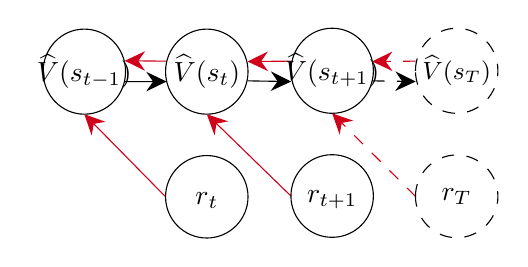
\begin{tikzpicture}[x=0.75pt,y=0.75pt,yscale=-1,xscale=1]
        
        %Straight Lines [id:da2592063600931961] 
        \draw [color={rgb, 255:red, 208; green, 2; blue, 27 }  ,draw opacity=1 ]   (282.5,135.16) -- (300.67,135.02) ;
        \draw [shift={(279.5,135.18)}, rotate = 359.55] [fill={rgb, 255:red, 208; green, 2; blue, 27 }  ,fill opacity=1 ][line width=0.08]  [draw opacity=0] (9.82,-4.72) -- (0,0) -- (9.82,4.72) -- (6.52,0) -- cycle    ;
        %Straight Lines [id:da41585806917853485] 
        \draw [color={rgb, 255:red, 208; green, 2; blue, 27 }  ,draw opacity=1 ]   (223.33,134.87) -- (240.67,135.02) ;
        \draw [shift={(220.33,134.85)}, rotate = 0.47] [fill={rgb, 255:red, 208; green, 2; blue, 27 }  ,fill opacity=1 ][line width=0.08]  [draw opacity=0] (9.82,-4.72) -- (0,0) -- (9.82,4.72) -- (6.52,0) -- cycle    ;
        %Shape: Ellipse [id:dp31493856088290983] 
        \draw   (181,140.07) .. controls (181,128.75) and (189.89,119.58) .. (200.86,119.58) .. controls (211.83,119.58) and (220.72,128.75) .. (220.72,140.07) .. controls (220.72,151.4) and (211.83,160.57) .. (200.86,160.57) .. controls (189.89,160.57) and (181,151.4) .. (181,140.07) -- cycle ;
        %Shape: Ellipse [id:dp5103941395609547] 
        \draw  [dash pattern={on 4.5pt off 4.5pt}] (360.4,139.66) .. controls (360.4,128.34) and (369.29,119.16) .. (380.26,119.16) .. controls (391.23,119.16) and (400.12,128.34) .. (400.12,139.66) .. controls (400.12,150.98) and (391.23,160.16) .. (380.26,160.16) .. controls (369.29,160.16) and (360.4,150.98) .. (360.4,139.66) -- cycle ;
        %Straight Lines [id:da30559831832260953] 
        \draw [color={rgb, 255:red, 0; green, 0; blue, 0 }  ,draw opacity=1 ]   (220.07,144.9) -- (237.5,144.86) ;
        \draw [shift={(240.5,144.85)}, rotate = 539.86] [fill={rgb, 255:red, 0; green, 0; blue, 0 }  ,fill opacity=1 ][line width=0.08]  [draw opacity=0] (9.82,-4.72) -- (0,0) -- (9.82,4.72) -- (6.52,0) -- cycle    ;
        %Shape: Ellipse [id:dp12377292733336898] 
        \draw  [color={rgb, 255:red, 0; green, 0; blue, 0 }  ,draw opacity=1 ] (240,140.07) .. controls (240,128.75) and (248.89,119.58) .. (259.86,119.58) .. controls (270.83,119.58) and (279.72,128.75) .. (279.72,140.07) .. controls (279.72,151.4) and (270.83,160.57) .. (259.86,160.57) .. controls (248.89,160.57) and (240,151.4) .. (240,140.07) -- cycle ;
        %Shape: Ellipse [id:dp9248757796917767] 
        \draw   (300.4,139.66) .. controls (300.4,128.34) and (309.29,119.16) .. (320.26,119.16) .. controls (331.23,119.16) and (340.12,128.34) .. (340.12,139.66) .. controls (340.12,150.98) and (331.23,160.16) .. (320.26,160.16) .. controls (309.29,160.16) and (300.4,150.98) .. (300.4,139.66) -- cycle ;
        %Straight Lines [id:da050274800713848156] 
        \draw [color={rgb, 255:red, 208; green, 2; blue, 27 }  ,draw opacity=1 ]   (202.96,162.71) -- (240,200.37) ;
        \draw [shift={(200.86,160.57)}, rotate = 45.48] [fill={rgb, 255:red, 208; green, 2; blue, 27 }  ,fill opacity=1 ][line width=0.08]  [draw opacity=0] (9.82,-4.72) -- (0,0) -- (9.82,4.72) -- (6.52,0) -- cycle    ;
        %Straight Lines [id:da7059353635730191] 
        \draw [color={rgb, 255:red, 208; green, 2; blue, 27 }  ,draw opacity=1 ]   (262.01,162.66) -- (300.4,200) ;
        \draw [shift={(259.86,160.57)}, rotate = 44.2] [fill={rgb, 255:red, 208; green, 2; blue, 27 }  ,fill opacity=1 ][line width=0.08]  [draw opacity=0] (9.82,-4.72) -- (0,0) -- (9.82,4.72) -- (6.52,0) -- cycle    ;
        %Straight Lines [id:da17885982011746426] 
        \draw [color={rgb, 255:red, 208; green, 2; blue, 27 }  ,draw opacity=1 ] [dash pattern={on 4.5pt off 4.5pt}]  (322.38,162.28) -- (360.4,200.16) ;
        \draw [shift={(320.26,160.16)}, rotate = 44.9] [fill={rgb, 255:red, 208; green, 2; blue, 27 }  ,fill opacity=1 ][line width=0.08]  [draw opacity=0] (9.82,-4.72) -- (0,0) -- (9.82,4.72) -- (6.52,0) -- cycle    ;
        %Shape: Ellipse [id:dp3523005799699832] 
        \draw  [dash pattern={on 4.5pt off 4.5pt}] (360.4,200.16) .. controls (360.4,189.16) and (369.29,180.23) .. (380.26,180.23) .. controls (391.23,180.23) and (400.12,189.16) .. (400.12,200.16) .. controls (400.12,211.17) and (391.23,220.09) .. (380.26,220.09) .. controls (369.29,220.09) and (360.4,211.17) .. (360.4,200.16) -- cycle ;
        %Shape: Ellipse [id:dp3509500153089894] 
        \draw   (300.4,200) .. controls (300.4,189) and (309.29,180.09) .. (320.26,180.09) .. controls (331.23,180.09) and (340.12,189) .. (340.12,200) .. controls (340.12,210.99) and (331.23,219.9) .. (320.26,219.9) .. controls (309.29,219.9) and (300.4,210.99) .. (300.4,200) -- cycle ;
        %Shape: Ellipse [id:dp17336392317383575] 
        \draw  [color={rgb, 255:red, 0; green, 0; blue, 0 }  ,draw opacity=1 ] (240,200.37) .. controls (240,189.4) and (248.89,180.5) .. (259.86,180.5) .. controls (270.83,180.5) and (279.72,189.4) .. (279.72,200.37) .. controls (279.72,211.34) and (270.83,220.23) .. (259.86,220.23) .. controls (248.89,220.23) and (240,211.34) .. (240,200.37) -- cycle ;
        %Straight Lines [id:da21459790152477998] 
        \draw [color={rgb, 255:red, 0; green, 0; blue, 0 }  ,draw opacity=1 ]   (279.5,144.52) -- (297.5,144.8) ;
        \draw [shift={(300.5,144.85)}, rotate = 180.91] [fill={rgb, 255:red, 0; green, 0; blue, 0 }  ,fill opacity=1 ][line width=0.08]  [draw opacity=0] (9.82,-4.72) -- (0,0) -- (9.82,4.72) -- (6.52,0) -- cycle    ;
        %Straight Lines [id:da8588950475203374] 
        \draw [color={rgb, 255:red, 208; green, 2; blue, 27 }  ,draw opacity=1 ] [dash pattern={on 4.5pt off 4.5pt}]  (342.5,135.16) -- (360.67,135.02) ;
        \draw [shift={(339.5,135.18)}, rotate = 359.55] [fill={rgb, 255:red, 208; green, 2; blue, 27 }  ,fill opacity=1 ][line width=0.08]  [draw opacity=0] (9.82,-4.72) -- (0,0) -- (9.82,4.72) -- (6.52,0) -- cycle    ;
        %Straight Lines [id:da9169375689094925] 
        \draw [color={rgb, 255:red, 0; green, 0; blue, 0 }  ,draw opacity=1 ] [dash pattern={on 4.5pt off 4.5pt}]  (339.5,144.52) -- (357.5,144.8) ;
        \draw [shift={(360.5,144.85)}, rotate = 180.91] [fill={rgb, 255:red, 0; green, 0; blue, 0 }  ,fill opacity=1 ][line width=0.08]  [draw opacity=0] (9.82,-4.72) -- (0,0) -- (9.82,4.72) -- (6.52,0) -- cycle    ;
        
        % Text Node
        \draw (320.26,201.59) node    {$r_{t+1}$};
        % Text Node
        \draw (200.86,140.07) node    {$\widehat{V}(s_{t-1})$};
        % Text Node
        \draw (320.26,139.66) node    {$\widehat{V}(s_{t+1})$};
        % Text Node
        \draw (380.26,139.66) node  [font=\small]  {$\widehat{V}(s_{T})$};
        % Text Node
        \draw (259.86,202) node  [color={rgb, 255:red, 208; green, 9; blue, 2 }  ,opacity=1 ]  {$\textcolor[rgb]{0,0,0}{r}\textcolor[rgb]{0,0,0}{_{t}}$};
        % Text Node
        \draw (259.86,140.07) node  [color={rgb, 255:red, 208; green, 9; blue, 2 }  ,opacity=1 ]  {$\textcolor[rgb]{0,0,0}{\widehat{V}}\textcolor[rgb]{0,0,0}{(s_{t})}$};
        % Text Node
        \draw (380.26,200.16) node    {$r_{T}$};

        \end{tikzpicture}
    \end{adjustbox}
  \end{center}
\caption{\textbf{Graphical representation of TD Learning}. Red arrows indicate the flow of the computations for deriving $\delta$ and updating $\widehat{V}$ expressed by equations \ref{td_error} and \ref{td_update}. Black arrows instead indicate the changes of $\widehat{V}$ moving from $s$ to $s_{t+1}$. Solid circles indicate states which have already been observed while dashed ones represent future not-yet observed states.}
\label{fig: td_learning}
\end{figure}
McClure \textit{et. al.} proposed that incentive salience is represented by $V$ as defined in equation \ref{td_v} while the error signal expressed by equation \ref{td_error} represents the activity of dopaminergic neurons with the dual function of driving the attribution of incentive salience (through reward prediction error coding as specified in section \ref{incentive_salience}) and guiding the previously mentioned action selection process \cite{schultz1997neural,mcclure2003computational,o2003temporal}. However, in later work, Zhang \textit{et. al.} highlighted the fact that the model proposed by McClure \textit{et. al.} fails to take into account an important part of the original incentive salience hypothesis: the dynamic modulation produced by the individual's internal state (see section \ref{wanting}) \cite{toates1994comparing,mcclure2003computational,berridge2004motivation,zhang2009neural,tindell2009dynamic,berridge2012prediction}. Zhang \textit{et. al.} therefore proposed a modification of the original TD Learning model to include a modulatory factor $k \in [0, +\infty]$ which can enhance ($k > 1$), dampen or even revert ($k < 1$) previously learned incentive salience values
\begin{align}
    \label{zhang_td_v}
    V(s_t) = \mathbb{E}[\tilde{r}(r_{t+1},k_{t}) + \gamma V(s_{t+1})]
\end{align}
here $\tilde{r}(.,.)$ is a function of two variables and can assume either an additive or multiplicative form \footnote{See \cite{zhang2009neural} for detailed description of the two forms and their functional differences.}. The main difference between the approaches of McClure \textit{et. al.} and Zhang \textit{et. al.} lies in the interpretation of $V$. Both authors see it as a combination of cached value (i.e. what has been learned from past experiences) and expectation over future $r$ but for McClure \textit{et. al.} all the future $r$ have the same weight while for Zhang \textit{et. al.} the state of the individual dynamically modulates the weighting of $r$. Using the notation from section \ref{incentive_salience}, we can say that the interaction $s$ between $I$ and $O$ at time $t_{+1}$ arises from the $V$ (i.e. incentive salience) generated after $s_{t}$. The mismatch between the predicted amount of reward and the actual reward received at time $t_{+1}$ generates an error signal that allows $I$ to learn about the "correct" magnitude of $V(s_{t})$ \cite{schultz2017reward} . As an example, an individual may anticipate that eating their favourite meal would be a rewarding experience but instead (for some reason) it was underwhelming. They therefore reduce the salience previously attributed to it. Importantly, $V(s_{t})$ does not just encompass the previous history of interactions between an individual and an object but also the current state of the individual themselves: the individual has learned from long experience that eating is a pleasurable activity but currently, since they are sated they do not expect much reward from doing it again in the near future.  \\
\\
In this view, motivation can be described as a mechanism that guides the interaction between individuals and objects. It controls and selects behaviours which are expected to lead to pleasurable outcomes for the individual (i.e. incentives or reward). These expectancies are the product of a learning process that can be modulated by the internal state of the individual. Therefore, from a behavioural point of view, an objects $O$ can acquire salience for an individual $I$ conditioned on its capacity to elicit rewarding experience $r$ \cite{berridge1998role,mcclure2003computational}. The amount of attributed salience is a valued representation of $O$ generated by $I$ and controls how likely and intense future interactions between the two will be. \cite{berridge1998role,mcclure2003computational}. Let $B$ represents the strength of an interaction between $I$ and $O$, $r$ a measure of how rewarding the interaction with $O$ is perceived to be and $V$ the generated attributed incentive salience.
\begin{figure}[h]
  \begin{center}
    \begin{adjustbox}{width=0.5\columnwidth}

        \tikzset{every picture/.style={line width=0.75pt}}
        
        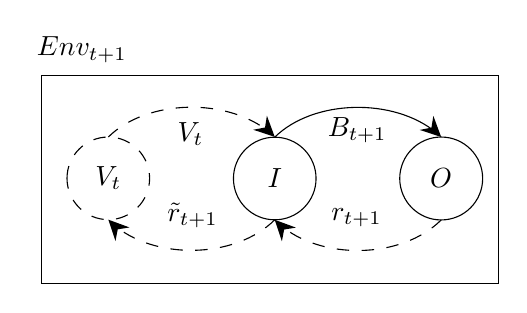
\begin{tikzpicture}[x=0.75pt,y=0.75pt,yscale=-1,xscale=1]
        
        %Shape: Circle [id:dp8739177923629333] 
        \draw   (123.48,130.05) .. controls (123.48,119.06) and (132.39,110.15) .. (143.38,110.15) .. controls (154.37,110.15) and (163.28,119.06) .. (163.28,130.05) .. controls (163.28,141.04) and (154.37,149.95) .. (143.38,149.95) .. controls (132.39,149.95) and (123.48,141.04) .. (123.48,130.05) -- cycle ;
        %Curve Lines [id:da2726669379173874] 
        \draw    (143.38,110.15) .. controls (161.99,91.83) and (200.82,90.88) .. (221.41,108.12) ;
        \draw [shift={(223.57,110.07)}, rotate = 224.02] [fill={rgb, 255:red, 0; green, 0; blue, 0 }  ][line width=0.08]  [draw opacity=0] (9.82,-4.72) -- (0,0) -- (9.82,4.72) -- (6.52,0) -- cycle    ;
        %Curve Lines [id:da4485667818478689] 
        \draw  [dash pattern={on 4.5pt off 4.5pt}]  (223.57,150.02) .. controls (204.36,169.14) and (165.2,169.5) .. (145.45,151.93) ;
        \draw [shift={(143.38,149.95)}, rotate = 405.89] [fill={rgb, 255:red, 0; green, 0; blue, 0 }  ][line width=0.08]  [draw opacity=0] (9.82,-4.72) -- (0,0) -- (9.82,4.72) -- (6.52,0) -- cycle    ;
        %Shape: Circle [id:dp8060688469385651] 
        \draw   (203.6,130.05) .. controls (203.6,119.01) and (212.54,110.07) .. (223.57,110.07) .. controls (234.6,110.07) and (243.55,119.01) .. (243.55,130.05) .. controls (243.55,141.08) and (234.6,150.02) .. (223.57,150.02) .. controls (212.54,150.02) and (203.6,141.08) .. (203.6,130.05) -- cycle ;
        %Shape: Rectangle [id:dp6054697635081123] 
        \draw   (31.2,80.5) -- (251.2,80.5) -- (251.2,180.83) -- (31.2,180.83) -- cycle ;
        %Shape: Circle [id:dp6091430023771998] 
        \draw  [dash pattern={on 4.5pt off 4.5pt}] (43.29,129.97) .. controls (43.29,118.98) and (52.2,110.07) .. (63.19,110.07) .. controls (74.18,110.07) and (83.09,118.98) .. (83.09,129.97) .. controls (83.09,140.96) and (74.18,149.87) .. (63.19,149.87) .. controls (52.2,149.87) and (43.29,140.96) .. (43.29,129.97) -- cycle ;
        %Curve Lines [id:da9876749075069771] 
        \draw  [dash pattern={on 4.5pt off 4.5pt}]  (143.38,149.95) .. controls (124.17,169.06) and (85.01,169.42) .. (65.26,151.85) ;
        \draw [shift={(63.19,149.87)}, rotate = 405.89] [fill={rgb, 255:red, 0; green, 0; blue, 0 }  ][line width=0.08]  [draw opacity=0] (9.82,-4.72) -- (0,0) -- (9.82,4.72) -- (6.52,0) -- cycle    ;
        %Curve Lines [id:da9412329086480583] 
        \draw  [dash pattern={on 4.5pt off 4.5pt}]  (63.19,110.07) .. controls (81.8,91.76) and (120.63,90.8) .. (141.21,108.05) ;
        \draw [shift={(143.38,110)}, rotate = 224.02] [fill={rgb, 255:red, 0; green, 0; blue, 0 }  ][line width=0.08]  [draw opacity=0] (9.82,-4.72) -- (0,0) -- (9.82,4.72) -- (6.52,0) -- cycle    ;
        
        % Text Node
        \draw (143.38,130.05) node  [font=\normalsize]  {$I$};
        % Text Node
        \draw (223.57,130.05) node  [font=\normalsize]  {$O$};
        % Text Node
        \draw (183.14,106.95) node  [font=\normalsize]  {$B_{t+1}$};
        % Text Node
        \draw (182.81,148.81) node  [font=\normalsize]  {$r_{t+1}$};
        % Text Node
        \draw (50.45,68.01) node  [font=\normalsize,rotate=-0.16]  {$Env_{t+1}$};
        % Text Node
        \draw (63.19,129.97) node  [font=\normalsize]  {$V_{t}$};
        % Text Node
        \draw (103.81,147.81) node  [font=\normalsize]  {$\tilde{r}_{t+1}$};
        % Text Node
        \draw (102.81,108.81) node  [font=\normalsize]  {$V_{t}$};
        \end{tikzpicture}
    \end{adjustbox}
  \end{center}
\caption[\textbf{The process of incentive salience attribution}]{Solid and dashed elements represent respectively observable (i.e. behavioural) and latent aspects of the process. The individual and the object that they interact with are indicated by $I$ and $O$. The strength of the interaction is represented by $B$. The salience that $I$ attributes to $O$ is expressed by $V$ while $r$ and $\tilde{r}$ are the experienced reward and its weighted version produced by the state of $I$. All the contextual factors influencing both the amount of $r$ perceived and the magnitude of $B$ produced are represented by $Env$. The dynamical natures of the process is expressed though the arbitrary temporal unit $t$.}
\label{fig: incs}
\end{figure}
Following Figure \ref{fig: incs}, at time $t+1$ an individual will produce an interaction with an object of strength $B$ according to the previous $V_{t}$. If we recall from section \ref{learning}, this process relies heavily on learning mechanisms making $V$ by nature dynamic and mutable. It should be noted that $B$ can be represented as a multidimensional variable defined by the instrumental behaviours conventionally used for assessing the \emph{wanting} component in animal studies (e.g. frequency, amount and duration of feeding behaviours like bites, nibbles and sniffs) \cite{berridge1998role}. During and after the interaction $I$ will experience a variable degree of reward $r_{t+1}$ that, weighted by their internal state, will then be used for updating $V_{t}$.  It is worth noting that the individual's internal state is not the only factor involved in the modulation of $r$, also the context in which $I$ and $O$ interact ($Env_{t+1}$ in Figure \ref{fig: incs}) seems to contribute to this \cite{palminteri2015contextual}. Following the idea presented in section \ref{manifold_rep_incentive_salience}, the latent state defined by $V$ could be represented as a manifold defined by the activity of those regions responsible for the attribution of incentive salience. Moreover, given the strong coupling between attributed incentive salience and behaviour \cite{berridge1998role} we would also expect the structure of this manifold to be a suitable descriptor of the behavioural aspects of attributed incentive salience.

\paragraph*{\textbf{From TD to Supervised Learning}}
\label{td_to_supervised}The approaches discussed above frame the estimation of attributed incentive salience as a reinforcement learning task. This requires the simulation of a sequence of interactions between $I$ and $O$ and the concomitant delivery of $r$  \cite{schultz1997neural,mcclure2003computational,zhang2009neural}. However, it is not always straightforward to replicate these interactions in real world scenarios, especially when dealing with human participants. The control on the internal state of $I$ and amount of $r$ delivered that McClure and Zhang assume is usually based on strict assumptions and can be achieved only in controlled experimental settings \cite{mcclure2003computational,zhang2009neural}. As an alternative solution for inferring $V$ outside the laboratory we propose to learn its manifold structure through supervised learning. Differently to what reported in the literature \cite{calhoun2019unsupervised, mccullough2021unsupervised, luxem2020identifying, pereira2020quantifying, shi2021learning} we argue that in this case the use of supervised in place of un-supervised techniques is to be preferred. Indeed, since we are dealing exclusively with behavioural data and trying to solve an inverse problem  we would like to learn a manifold structure which is not just a generic indicator of behavioural phenotype \cite{luxem2020identifying} but also obeys to specific functional constrains.\\
\\
In this approach, an experimenter gathers data on a set of interactions between $I$ and $O$ and let a learning algorithm to estimate two functions:
\begin{gather}
\label{supervised_v}
    V(s_{t}) = f^{1}(O, \tilde{r_{t}}, V(s_{t-1}); \theta^{1}) \\
    r_{t+1} = f^{2}(V(s_{t}); \theta^{2}) \nonumber
\end{gather}
here $f^{1}$ and $f^{2}$ are arbitrarily complex functions while $\theta^{1}$ and $\theta^{2}$ are parameters that the learning algorithm has to infer. The future reward that an individual expects after an interaction with an object is produced by the current level of attributed salience, which  itself is a function of the current internal state of the individual (expressed through the amount of reward just experienced) and the incentive salience previously attributed to the object. It is important to note that the two functions above need to be recursive over all $s \in S$ (see equations \ref{td_v} and \ref{zhang_td_v}) in order to provide $V(s_{t})$ with the dual purpose of caching all the past $V$ and being a suitable predictor for all the $r$. This formulation however still requires a measure of the $r$ experienced by $I$ (or more precisely its weighted version $\tilde{r}$) after interacting with $O$, which is not easily accessible. However, Thorndike's law of effect \cite{thorndike1927law} and Skinner's operant conditioning principles \cite{skinner1965science} suggest that $r$, which  like $V$ is a non observable latent variable, manifests itself through the intensity of interactions between $I$ and $O$ (i.e. $B$ in Figure \ref{fig: incs}): the frequency and amount of object-directed behaviours increase or decrease as a function of the rewards an individual expects to receive \cite{berridge2004motivation,schultz2017reward}. Since $V(s_{t})$ predicts how much $r$ an $I$ expects to receive from interacting with $O$, we should also expect the strength of their future interactions to be a function of $V(s_{t})$. This can be represented re-arranging the equations in \ref{supervised_v} in a more compact form as a chain of functions
\begin{align}
\label{supervised_b}
    B_{t+1} = f^{2}(f^{1}(O, B_{t}, V(s_{t-1}); \theta^{1});  \theta^{2})
\end{align}
To approximate the above expression, a learning algorithm would require records of behaviours generated by individuals while interacting with a diverse set of potentially rewarding objects. Here, we argue that video games are one way to obtain this type of data at scale while also achieving some level of ecological validity.

\subsection{Video Games and Telemetry}
\label{videogame_telemetries}
As we highlighted in chapter \ref{chapter_lit_review}, interacting with video games is a volitional activity driven largely by the capacity of the games to provide pleasurable experiences \cite{boyle2012engagement}. Behaviour within the game is best understood as the result of a value attribution process similar to that of secondary reward objects (see section \ref{incentive_salience}). Indeed, it appears that the play behaviour is often produced and maintained by the structural characteristics of the game (e.g. game mechanics) \cite{king2010video} which, working like conventional reinforcement mechanisms \cite{chumbley2006affect,wang2011game,phillips2013videogame,avserivskis2017computational}, produce effects similar to operant conditioning \cite{skinner1965science}. Although caution should be applied when complex activities are investigated using neuroimaging techniques, evidence suggest that the maintenance of video games playing behaviour engages the same cortico-striatal structures \cite{hoeft2008gender,mathiak2011reward,cole2012interactivity,klasen2012neural,lorenz2015video,gleich2017functional} and neurotransmitters \cite{koepp1998evidence} involved in reward processing. This, seems also supported at the behavioural level where the ammount of experienced in-game reward appears to play a role in controlling how likely is an individual to keep engaging in playing behaviour \cite{agarwal2017quitting, steyvers2019joint}. This, in conjunction with a growing literature highlighting similarities between certain video game mechanics and activities driven by secondary rewards (e.g. gambling) \cite{king2010role,drummond2018video,zendle2018video}, corroborates the idea that video games are able to elicit behavioural responses through incentive mechanics. In this view, video games with different structural characteristics could be seen as objects possessing rewarding properties that heavily depend on the individuals interacting with them (e.g. an individual's preference for a specific game mechanic). Hence, similarly to the process specified in chapter \ref{chapter_lit_review}, we can expect that through repeated interactions, an individual will experience varying degrees of reward determined by their internal state and the characteristics of the game. These interactions will produce continuous adjustments in the level of saliency attributed to playing that specific game which in turn will influence the frequency and amount of future interactions with that same game. Other than offering a context for observing the process of incentive salience attribution, video games allow us to obtain large volumes of behavioural data (similar to those mentioned in chapter \ref{chapter_lit_review}) in a naturalistic fashion. This is made possible by the widespread practice of obtaining high frequency records (i.e. telemetry\footnote{See \cite{el2016game} for a more technical description of telemetry in video games.}) of players' behaviour during the game \cite{drachen2015behavioral}. This approach, despite offering less control and rigour than conventional experimental procedures, allows us to obtain a more faithful representation of natural behaviour (similarly to field studies) while avoiding some of the limitations connected with laboratory-based studies (e.g. sampling and observer biases).
\newline
\newline
In order to use this type of behavioural data to model attributed incentive salience, a learning algorithm should possess the following properties. First, it should be scalable and noise resilient, to leverage large volumes of naturalistic data in an efficient and effective manner. Second, it should be able to approximate arbitrarily complex functions, given that the shape of the functions specified in equation \ref{td_to_supervised} is not known a-priori. And finally, it should be able to produce an approximation of $V(s_{t})$ that can be inspected in order to evaluate if its functional properties can be compared with those of attributed incentive salience. Artificial Neural Networks (ANNs) appear to satisfy these requirements.

\subsection{Artificial Neural Networks}
\label{artificial_neural_networks}
In their conventional form, ANNs can be seen as chains of nested functions (the layers of the network). These layers are vector valued (there are multiple units or neurons in each layer) and organized as directed acyclic computational graphs (information only flows forward). When the number of layers is greater than two, the prefix "deep" is usually applied \cite{bengio2017deep}. The goal of this ensemble of functions is to create a mapping between an input $x$ and a target $y$. Following the example illustrated in Figure \ref{fig: ffnn}, given the set of parameters $\Theta = \{\theta^1, \theta^2 \}$ an ANN would first infer a function $h = f(x;\theta^{1})$, mapping the input to a new representation $h$. The same representation $h$ would then become the input of a second function $\widehat{y} = f^{1}(h;\theta^{2})$ which produces an estimate of the target \cite{bengio2017deep}. In this sense, we can think of each layer as a collection of many non-linear vector to scalar functions taking the previous layer as input and generating the units for the layer that follows \cite{bengio2017deep}. By increasing the number of layers and units, ANNs can approximate an extremely large class of functions \cite{rumelhart1986learning}.
\begin{figure}
    \begin{center}
        \begin{adjustbox}{width=0.4\textwidth}
            \tikzset{every picture/.style={line width=0.75pt}} %set default line width to 0.75pt        
            
            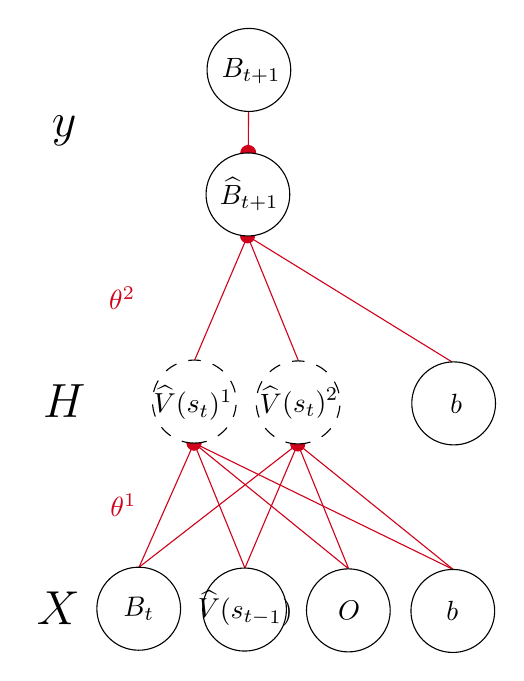
\begin{tikzpicture}[x=0.75pt,y=0.75pt,yscale=-1,xscale=1]
            %uncomment if require: \path (0,350); %set diagram left start at 0, and has height of 350
            
            %Straight Lines [id:da8866607252953388] 
            \draw [color={rgb, 255:red, 208; green, 2; blue, 27 }  ,draw opacity=1 ]   (227.88,279.44) -- (254.36,219.65) ;
            \draw [shift={(254.36,219.65)}, rotate = 293.89] [color={rgb, 255:red, 208; green, 2; blue, 27 }  ,draw opacity=1 ][fill={rgb, 255:red, 208; green, 2; blue, 27 }  ,fill opacity=1 ][line width=0.75]      (0, 0) circle [x radius= 3.02, y radius= 3.02]   ;
            %Straight Lines [id:da0731191645042184] 
            \draw [color={rgb, 255:red, 208; green, 2; blue, 27 }  ,draw opacity=1 ]   (254.68,179.65) -- (280.16,119.85) ;
            \draw [shift={(280.16,119.85)}, rotate = 293.08] [color={rgb, 255:red, 208; green, 2; blue, 27 }  ,draw opacity=1 ][fill={rgb, 255:red, 208; green, 2; blue, 27 }  ,fill opacity=1 ][line width=0.75]      (0, 0) circle [x radius= 3.02, y radius= 3.02]   ;
            %Straight Lines [id:da4826752085294559] 
            \draw [color={rgb, 255:red, 208; green, 2; blue, 27 }  ,draw opacity=1 ]   (304.68,180.05) -- (280.16,119.85) ;
            \draw [shift={(280.16,119.85)}, rotate = 247.84] [color={rgb, 255:red, 208; green, 2; blue, 27 }  ,draw opacity=1 ][fill={rgb, 255:red, 208; green, 2; blue, 27 }  ,fill opacity=1 ][line width=0.75]      (0, 0) circle [x radius= 2.01, y radius= 2.01]   ;
            %Straight Lines [id:da39539248901414714] 
            \draw [color={rgb, 255:red, 208; green, 2; blue, 27 }  ,draw opacity=1 ]   (328.88,280.25) -- (304.36,220.05) ;
            \draw [shift={(304.36,220.05)}, rotate = 247.84] [color={rgb, 255:red, 208; green, 2; blue, 27 }  ,draw opacity=1 ][fill={rgb, 255:red, 208; green, 2; blue, 27 }  ,fill opacity=1 ][line width=0.75]      (0, 0) circle [x radius= 3.02, y radius= 3.02]   ;
            %Straight Lines [id:da8990891706173756] 
            \draw [color={rgb, 255:red, 208; green, 2; blue, 27 }  ,draw opacity=1 ]   (278.88,279.85) -- (254.36,219.65) ;
            \draw [shift={(254.36,219.65)}, rotate = 247.84] [color={rgb, 255:red, 208; green, 2; blue, 27 }  ,draw opacity=1 ][fill={rgb, 255:red, 208; green, 2; blue, 27 }  ,fill opacity=1 ][line width=0.75]      (0, 0) circle [x radius= 3.02, y radius= 3.02]   ;
            %Straight Lines [id:da1147021220204143] 
            \draw [color={rgb, 255:red, 208; green, 2; blue, 27 }  ,draw opacity=1 ]   (328.88,280.25) -- (254.36,219.65) ;
            \draw [shift={(254.36,219.65)}, rotate = 219.12] [color={rgb, 255:red, 208; green, 2; blue, 27 }  ,draw opacity=1 ][fill={rgb, 255:red, 208; green, 2; blue, 27 }  ,fill opacity=1 ][line width=0.75]      (0, 0) circle [x radius= 3.02, y radius= 3.02]   ;
            %Straight Lines [id:da30405558125224674] 
            \draw [color={rgb, 255:red, 208; green, 2; blue, 27 }  ,draw opacity=1 ]   (278.88,279.85) -- (304.36,220.05) ;
            \draw [shift={(304.36,220.05)}, rotate = 293.08] [color={rgb, 255:red, 208; green, 2; blue, 27 }  ,draw opacity=1 ][fill={rgb, 255:red, 208; green, 2; blue, 27 }  ,fill opacity=1 ][line width=0.75]      (0, 0) circle [x radius= 3.02, y radius= 3.02]   ;
            %Straight Lines [id:da7841365763851936] 
            \draw [color={rgb, 255:red, 208; green, 2; blue, 27 }  ,draw opacity=1 ]   (227.88,279.44) -- (304.36,220.05) ;
            \draw [shift={(304.36,220.05)}, rotate = 322.17] [color={rgb, 255:red, 208; green, 2; blue, 27 }  ,draw opacity=1 ][fill={rgb, 255:red, 208; green, 2; blue, 27 }  ,fill opacity=1 ][line width=0.75]      (0, 0) circle [x radius= 3.02, y radius= 3.02]   ;
            %Straight Lines [id:da5618158283475858] 
            \draw [color={rgb, 255:red, 208; green, 2; blue, 27 }  ,draw opacity=1 ]   (379.21,280.52) -- (304.36,220.05) ;
            \draw [shift={(304.36,220.05)}, rotate = 218.93] [color={rgb, 255:red, 208; green, 2; blue, 27 }  ,draw opacity=1 ][fill={rgb, 255:red, 208; green, 2; blue, 27 }  ,fill opacity=1 ][line width=0.75]      (0, 0) circle [x radius= 3.02, y radius= 3.02]   ;
            %Straight Lines [id:da4509011415852858] 
            \draw [color={rgb, 255:red, 208; green, 2; blue, 27 }  ,draw opacity=1 ]   (378.61,180.51) -- (280.16,119.85) ;
            \draw [shift={(280.16,119.85)}, rotate = 211.64] [color={rgb, 255:red, 208; green, 2; blue, 27 }  ,draw opacity=1 ][fill={rgb, 255:red, 208; green, 2; blue, 27 }  ,fill opacity=1 ][line width=0.75]      (0, 0) circle [x radius= 3.02, y radius= 3.02]   ;
            %Straight Lines [id:da7242656967921071] 
            \draw [color={rgb, 255:red, 208; green, 2; blue, 27 }  ,draw opacity=1 ]   (379.21,280.52) -- (254.36,219.65) ;
            \draw [shift={(254.36,219.65)}, rotate = 205.99] [color={rgb, 255:red, 208; green, 2; blue, 27 }  ,draw opacity=1 ][fill={rgb, 255:red, 208; green, 2; blue, 27 }  ,fill opacity=1 ][line width=0.75]      (0, 0) circle [x radius= 3.02, y radius= 3.02]   ;
            %Shape: Ellipse [id:dp9097533963365589] 
            \draw  [fill={rgb, 255:red, 255; green, 255; blue, 255 }  ,fill opacity=1 ][dash pattern={on 4.5pt off 4.5pt}] (304.36,220.05) .. controls (293.22,219.96) and (284.26,210.94) .. (284.35,199.89) .. controls (284.44,188.84) and (293.54,179.96) .. (304.68,180.05) .. controls (315.82,180.14) and (324.77,189.17) .. (324.69,200.21) .. controls (324.6,211.26) and (315.5,220.14) .. (304.36,220.05) -- cycle ;
            %Shape: Ellipse [id:dp9467435778420286] 
            \draw  [fill={rgb, 255:red, 255; green, 255; blue, 255 }  ,fill opacity=1 ][dash pattern={on 4.5pt off 4.5pt}] (254.36,219.65) .. controls (243.22,219.56) and (234.27,210.53) .. (234.36,199.49) .. controls (234.44,188.44) and (243.54,179.56) .. (254.68,179.65) .. controls (265.82,179.74) and (274.78,188.77) .. (274.69,199.81) .. controls (274.6,210.86) and (265.5,219.74) .. (254.36,219.65) -- cycle ;
            %Shape: Ellipse [id:dp4514100854948462] 
            \draw  [fill={rgb, 255:red, 255; green, 255; blue, 255 }  ,fill opacity=1 ] (379.29,220.52) .. controls (368.15,220.43) and (359.2,211.4) .. (359.29,200.36) .. controls (359.37,189.31) and (368.47,180.43) .. (379.61,180.52) .. controls (390.75,180.61) and (399.71,189.64) .. (399.62,200.68) .. controls (399.53,211.73) and (390.43,220.61) .. (379.29,220.52) -- cycle ;
            %Shape: Ellipse [id:dp2836578028815524] 
            \draw  [fill={rgb, 255:red, 255; green, 255; blue, 255 }  ,fill opacity=1 ] (227.56,319.44) .. controls (216.42,319.35) and (207.46,310.32) .. (207.55,299.28) .. controls (207.64,288.23) and (216.74,279.35) .. (227.88,279.44) .. controls (239.02,279.53) and (247.97,288.56) .. (247.89,299.6) .. controls (247.8,310.65) and (238.7,319.53) .. (227.56,319.44) -- cycle ;
            %Shape: Ellipse [id:dp10987171532240936] 
            \draw  [fill={rgb, 255:red, 255; green, 255; blue, 255 }  ,fill opacity=1 ] (278.56,319.85) .. controls (267.42,319.76) and (258.46,310.73) .. (258.55,299.69) .. controls (258.64,288.64) and (267.74,279.76) .. (278.88,279.85) .. controls (290.02,279.94) and (298.97,288.96) .. (298.88,300.01) .. controls (298.79,311.06) and (289.69,319.94) .. (278.56,319.85) -- cycle ;
            %Shape: Ellipse [id:dp5734471221931936] 
            \draw  [fill={rgb, 255:red, 255; green, 255; blue, 255 }  ,fill opacity=1 ] (328.56,320.25) .. controls (317.42,320.16) and (308.46,311.13) .. (308.55,300.09) .. controls (308.64,289.04) and (317.74,280.16) .. (328.88,280.25) .. controls (340.01,280.34) and (348.97,289.37) .. (348.88,300.41) .. controls (348.79,311.46) and (339.69,320.34) .. (328.56,320.25) -- cycle ;
            %Shape: Ellipse [id:dp8405299754625457] 
            \draw  [fill={rgb, 255:red, 255; green, 255; blue, 255 }  ,fill opacity=1 ] (378.89,320.52) .. controls (367.75,320.43) and (358.79,311.4) .. (358.88,300.36) .. controls (358.97,289.31) and (368.07,280.43) .. (379.21,280.52) .. controls (390.35,280.61) and (399.3,289.64) .. (399.21,300.68) .. controls (399.13,311.73) and (390.03,320.61) .. (378.89,320.52) -- cycle ;
            %Straight Lines [id:da531681756338569] 
            \draw [color={rgb, 255:red, 208; green, 2; blue, 27 }  ,draw opacity=1 ]   (280.48,79.86) -- (280.64,59.86) ;
            \draw [shift={(280.48,79.86)}, rotate = 270.46] [color={rgb, 255:red, 208; green, 2; blue, 27 }  ,draw opacity=1 ][fill={rgb, 255:red, 208; green, 2; blue, 27 }  ,fill opacity=1 ][line width=0.75]      (0, 0) circle [x radius= 3.35, y radius= 3.35]   ;
            %Shape: Ellipse [id:dp7122318662628844] 
            \draw  [fill={rgb, 255:red, 255; green, 255; blue, 255 }  ,fill opacity=1 ] (280.64,59.86) .. controls (269.51,59.77) and (260.55,50.74) .. (260.64,39.69) .. controls (260.73,28.65) and (269.83,19.77) .. (280.97,19.86) .. controls (292.1,19.95) and (301.06,28.97) .. (300.97,40.02) .. controls (300.88,51.06) and (291.78,59.95) .. (280.64,59.86) -- cycle ;
            %Shape: Ellipse [id:dp8923679098088735] 
            \draw  [fill={rgb, 255:red, 255; green, 255; blue, 255 }  ,fill opacity=1 ] (280.16,119.85) .. controls (269.03,119.76) and (260.07,110.74) .. (260.16,99.69) .. controls (260.25,88.65) and (269.35,79.77) .. (280.48,79.86) .. controls (291.62,79.94) and (300.58,88.97) .. (300.49,100.02) .. controls (300.4,111.06) and (291.3,119.94) .. (280.16,119.85) -- cycle ;
            
            % Text Node
            \draw (279.05,299.33) node  [rotate=-0.94] [align=left] {$\displaystyle \widehat{V}(s_{t-1})$};
            % Text Node
            \draw (329.04,300.22) node  [rotate=-1.88] [align=left] {$\displaystyle O$};
            % Text Node
            \draw (378.8,300.47) node  [rotate=-359.63] [align=left] {$\displaystyle b$};
            % Text Node
            \draw (380.6,200.87) node  [rotate=-358.65] [align=left] {$\displaystyle b$};
            % Text Node
            \draw (253.92,200.36) node  [rotate=-0.88] [align=left] {$\displaystyle \widehat{V}(s_{t})^1$};
            % Text Node
            \draw (305.05,199.96) node  [rotate=-358.47] [align=left] {$\displaystyle \widehat{V}(s_{t})^2$};
            % Text Node
            \draw (280.95,99.59) node  [rotate=-359.67] [align=left] {$\displaystyle \widehat{B}_{t+1}$};
            % Text Node
            \draw (189,299.2) node  [font=\LARGE,rotate=-0.33]  {$X$};
            % Text Node
            \draw (191.8,199.22) node  [font=\LARGE,rotate=-359.71]  {$H$};
            % Text Node
            \draw (191.84,69.22) node  [font=\LARGE,rotate=-0.13]  {$y$};
            % Text Node
            \draw (220.4,249.43) node  [font=\normalsize,color={rgb, 255:red, 0; green, 0; blue, 0 }  ,opacity=1 ,rotate=-359.94]  {$\textcolor[rgb]{0.82,0.01,0.11}{\theta }\textcolor[rgb]{0.82,0.01,0.11}{^{1}}$};
            % Text Node
            \draw (219.7,149.93) node  [font=\normalsize,color={rgb, 255:red, 208; green, 2; blue, 27 }  ,opacity=1 ,rotate=-359.3]  {$\textcolor[rgb]{0.82,0.01,0.11}{\theta }\textcolor[rgb]{0.82,0.01,0.11}{^{2}}$};
            % Text Node
            \draw (227.72,299.44) node  [rotate=-358] [align=left] {$\displaystyle B_{t}$};
            % Text Node
            \draw (281.85,40.31) node  [rotate=-359.39] [align=left] {$\displaystyle B_{t+1}$};
            
            
            \end{tikzpicture}
        \end{adjustbox}
    \end{center}
\caption[\textbf{Feedforward ANN with a 2-units hidden layer}]{The figure represents how a feedforward ANN could be used for estimating $V(s_t)$ given a sequence of observed behaviors ($B$) produced while interacting with an object ($O$). Here $X$ and $H$ indicates the model's input and the inferred representation.  $y$ indicates both the target and the estimate produced by the model while $b$ is a bias term. The collection of all the red lines indicates the $\Theta$ that the ANN has to estimate while each line represents a single parameter $w$ or $b$. The circles are computational units (i.e. artificial neurons) whose outputs are given by $\phi(W_i^ \top X+ b )$. Here, $\phi$ is a non-linear function conventionally called activation, $W_i$ the weight matrix for the $i^{th}$ unit, $b$ the bias vector and $X$ the output from the previous layer.}
\label{fig: ffnn}
\end{figure}
An ANN finds the optimal values for $\Theta$ by taking forward and a backward passes through the computational graph. In the forward pass, information flows from the input $x$ to the estimate $\widehat{y}$ according to the operations specified in Figure \ref{fig: ffnn}. During the backward pass, the error between $\widehat{y}$ and the target is first computed
\begin{gather}
\label{loss}
    \mathcal{L} = l(y, \widehat{y})
\end{gather}
Here $l$ is a generic convex and differentiable function measuring the distance between $y$ and $\widehat{y}$. Then, the gradient of the error with respect to all the parameters is found and an update is performed taking steps of size $\alpha \in [0, 1]$ in the direction opposite to the gradient
\begin{gather}
\label{delta_rule}
    \Delta w^{j}_{i} = -\alpha\frac{\partial \mathcal{L}}{\partial w^{j}_{i}} \\
    w^{j}_{i} \leftarrow w^{j}_{i} + \Delta w^{j}_{i} \nonumber
\end{gather}
What we illustrated here is the application of the delta rule for updating the $i^{th}$ parameter of the $j^{th}$ layer through gradient descent \cite{widrow1960adaptive}. Deep feedforward ANNs rely on a generalization of this rule (i.e. backpropagation \cite{rumelhart1986learning}) for efficiently computing the gradient for all the parameters in the network.  
\\
\\
Returning to the supervised learning problem specified in section \ref{td_to_supervised}, a feedforward ANN approximates $V(s_{t})$ by mapping the inputs of equation \ref{supervised_b} to a candidate $\widehat{V}(s_{t})$ which is then used to generate an estimate $\widehat{B}_{t+1}$. Then, during the backward pass $\widehat{V}(s_{t})$ is adjusted based on the degree of mismatch between the estimation that it produced and the real value of $B_{t+1}$. It is of interest to note that there is a certain degree of overlap between how ANNs adjust their weights and the TD update illustrated in section \ref{td_learning}. Indeed, in single-step scenarios (i.e. predicting $s_{t+1}$ based on $s_{t}$ for each $s \in S$) the parameter changes produced by the two methods are the same \cite{sutton1988learning}. The major difference lies in the delivery of the update: TD learning performs it at every step while backpropagation-based algorithms must  wait until the end of the sequence in order to collate all the observed errors in a single term \cite{sutton1988learning}.

\paragraph*{\textbf{Recurrent Neural Networks}}
\label{rnn_theory}
Despite their universal function approximation properties \cite{hornik1989multilayer}, feedforward ANNs are not suitable for the type of recursive operations expressed in paragraph \ref{td_to_supervised} \cite{bengio2017deep}. As we can see from Figure \ref{fig: ffnn_rnn}A, given a sequence of inputs and targets, a conventional feedforward ANN would be limited to learning a temporally local function of the form
\begin{gather}
\label{td_ffnn}
    B_{t+1} = f^2(f^1(O, B_{t}; \theta^{1}); \theta^{2})
\end{gather}
Even when $\Theta$ are shared across time, the estimated $\widehat{V}(s_t)$ cannot incorporate information from past $\widehat{V}(s)$ nor guarantee predictive power for the future $B$. A solution to this problem is offered by ANNs with feedback connections like Recurrent Neural Networks (RNNs). These  are a class of ANNs that are able to efficiently process long sequences of data while also relaxing the requirements of conventional feedforward ANNs for fixed length inputs \cite{bengio2017deep}. Looking at Figure \ref{fig: ffnn_rnn}B, we see that for each $t \in T$ a RNN would compute $\widehat{V}(s_t)$ using both the input $OB_{t}$ and the previously estimated representation $\widehat{V}(s_{t-1})$. This, in combination with the recursive application of $\Theta$, allows the network to learn a function over the entire temporal sequence and to provide $\widehat{V}(s_t)$ with the desirable properties mentioned in section \ref{td_to_supervised}. The structure of $\Theta$ is more complex in RNNs than in feedforward ANNs \footnote{See \cite{bengio2017deep} for a description of the parameters' structure in RNNs.} and a detailed derivation of the underlying optimization process is outside the scope of the present work. Nevertheless, it is worth singling out how the recurrent nature of the computations underlying the generation of $\widehat{V}(s_t)$  makes RNNs suitable for approximating the function specified in section \ref{td_to_supervised}. \\
\\
Following Figure \ref{fig: ffnn_rnn}B, let $\widehat{V}(s_t)$ be the representation inferred by the model at time $t$ and its associated parameters. Optimal parameter values are found through the same update rule used in feedforward ANNs
\begin{gather}
\label{bptt_1}
    \widehat{V}(s_t) \leftarrow \widehat{V}(s_t) + -\alpha \frac{\partial \mathcal{L}}{\partial \widehat{V}(s_t)}
\end{gather}
however, since $\mathcal{L}$ can now only be observed at the end of a temporal sequence, computing $\frac{\partial \mathcal{L}}{\partial \widehat{V}(s_t)}$ requires us to take into account all the intermediate steps from $t$ to $T$. This is achieved applying the chain rule and propagating the error gradient backward in time \cite{bengio2017deep,lillicrap2019backpropagation}
\begin{gather}
\label{bptt_2}
    \frac{\partial \mathcal{L}}{\partial \widehat{V}(s_t)} = 
    \frac{\partial \mathcal{L}}{\partial \widehat{V}(s_{T})}
    \frac{\partial \widehat{V}(s_{T})}{\partial \widehat{V}(s_{T-1})}
    \dots
    \frac{\partial \widehat{V}(s_{T-n})}{\partial \widehat{V}(s_{t})}
\end{gather}
This implies that, similarly to TD update, the error flow forces $\widehat{V}(s_t)$ to retain information from $OB_t$ and $\widehat{V}(s_{t-1})$ in order to perform estimation of $B_{t+1}$ while still being useful for generating $\widehat{V}(s_{t+1})$ as we can see from Figure \ref{fig: ffnn_rnn}B. This process is made more efficient by an RNN variant called Long Short-Term Memory (LSTM) \cite{hochreiter1997long}, which, as well as improving the propagation of the error gradient, has specialized mechanisms for inferring, at each point in time, which portion of information should be kept or discarded in order to minimize $\mathcal{L}$ \cite{hochreiter1997long,bengio2017deep}.
\begin{figure}[h]
\begin{center}
\begin{adjustbox}{width=0.5\columnwidth}
    \tikzset{every picture/.style={line width=0.75pt}} %set default line width to 0.75pt        
    
    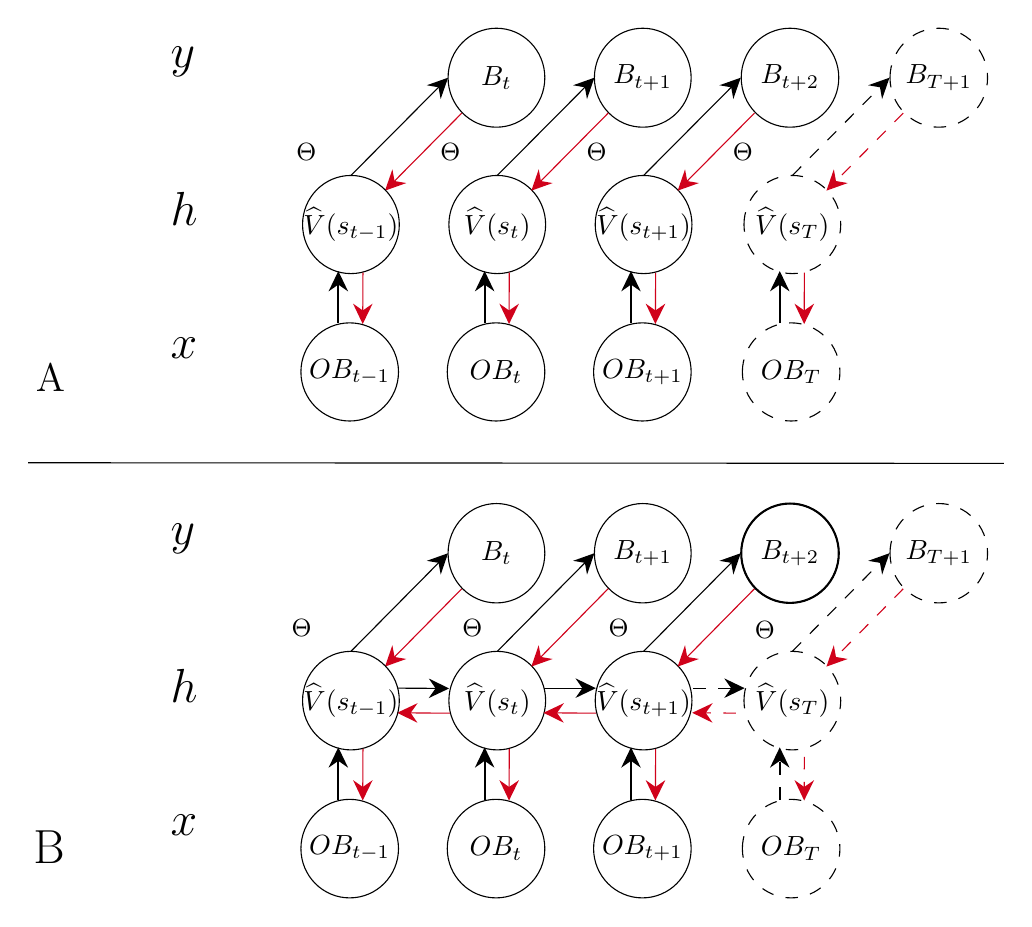
\begin{tikzpicture}[x=0.75pt,y=0.75pt,yscale=-1,xscale=1]
    %uncomment if require: \path (0,432); %set diagram left start at 0, and has height of 432
    
    %Shape: Ellipse [id:dp9152556376471453] 
    \draw   (252.87,325.26) .. controls (252.87,312.15) and (263.3,301.52) .. (276.18,301.52) .. controls (289.05,301.52) and (299.48,312.15) .. (299.48,325.26) .. controls (299.48,338.37) and (289.05,349) .. (276.18,349) .. controls (263.3,349) and (252.87,338.37) .. (252.87,325.26) -- cycle ;
    %Straight Lines [id:da0084456304461753] 
    \draw [color={rgb, 255:red, 208; green, 2; blue, 27 }  ,draw opacity=1 ]   (230.94,331.15) -- (253.32,331.31) ;
    \draw [shift={(227.94,331.12)}, rotate = 0.43] [fill={rgb, 255:red, 208; green, 2; blue, 27 }  ,fill opacity=1 ][line width=0.08]  [draw opacity=0] (9.82,-4.72) -- (0,0) -- (9.82,4.72) -- (6.52,0) -- cycle    ;
    %Shape: Ellipse [id:dp18326344407352502] 
    \draw   (181.58,396.56) .. controls (181.58,383.45) and (192.11,372.82) .. (205.08,372.82) .. controls (218.06,372.82) and (228.59,383.45) .. (228.59,396.56) .. controls (228.59,409.67) and (218.06,420.3) .. (205.08,420.3) .. controls (192.11,420.3) and (181.58,409.67) .. (181.58,396.56) -- cycle ;
    %Shape: Ellipse [id:dp4732045107682973] 
    \draw   (252.09,396.56) .. controls (252.09,383.45) and (262.61,372.82) .. (275.59,372.82) .. controls (288.57,372.82) and (299.09,383.45) .. (299.09,396.56) .. controls (299.09,409.67) and (288.57,420.3) .. (275.59,420.3) .. controls (262.61,420.3) and (252.09,409.67) .. (252.09,396.56) -- cycle ;
    %Straight Lines [id:da9106304988340169] 
    \draw    (205.67,301.52) -- (250.37,256.37) ;
    \draw [shift={(252.48,254.24)}, rotate = 494.71] [fill={rgb, 255:red, 0; green, 0; blue, 0 }  ][line width=0.08]  [draw opacity=0] (9.82,-4.72) -- (0,0) -- (9.82,4.72) -- (6.52,0) -- cycle    ;
    %Straight Lines [id:da5186602107869037] 
    \draw [color={rgb, 255:red, 208; green, 2; blue, 27 }  ,draw opacity=1 ]   (259.09,271.36) -- (224.2,306.73) ;
    \draw [shift={(222.1,308.86)}, rotate = 314.62] [fill={rgb, 255:red, 208; green, 2; blue, 27 }  ,fill opacity=1 ][line width=0.08]  [draw opacity=0] (9.82,-4.72) -- (0,0) -- (9.82,4.72) -- (6.52,0) -- cycle    ;
    %Shape: Ellipse [id:dp6434768624828036] 
    \draw   (322.59,396.56) .. controls (322.59,383.45) and (333.11,372.82) .. (346.09,372.82) .. controls (359.07,372.82) and (369.59,383.45) .. (369.59,396.56) .. controls (369.59,409.67) and (359.07,420.3) .. (346.09,420.3) .. controls (333.11,420.3) and (322.59,409.67) .. (322.59,396.56) -- cycle ;
    %Shape: Ellipse [id:dp4847846412537088] 
    \draw   (252.48,254.24) .. controls (252.48,241.02) and (262.91,230.3) .. (275.78,230.3) .. controls (288.65,230.3) and (299.09,241.02) .. (299.09,254.24) .. controls (299.09,267.46) and (288.65,278.18) .. (275.78,278.18) .. controls (262.91,278.18) and (252.48,267.46) .. (252.48,254.24) -- cycle ;
    %Shape: Ellipse [id:dp07973567399208026] 
    \draw   (322.98,254.24) .. controls (322.98,241.02) and (333.42,230.3) .. (346.29,230.3) .. controls (359.16,230.3) and (369.59,241.02) .. (369.59,254.24) .. controls (369.59,267.46) and (359.16,278.18) .. (346.29,278.18) .. controls (333.42,278.18) and (322.98,267.46) .. (322.98,254.24) -- cycle ;
    %Shape: Ellipse [id:dp05423142626898558] 
    \draw   (393.72,254.24) .. controls (393.72,241.02) and (404.24,230.3) .. (417.22,230.3) .. controls (430.2,230.3) and (440.72,241.02) .. (440.72,254.24) .. controls (440.72,267.46) and (430.2,278.18) .. (417.22,278.18) .. controls (404.24,278.18) and (393.72,267.46) .. (393.72,254.24) -- cycle ;
    %Shape: Ellipse [id:dp22782348689960996] 
    \draw   (182.37,325.26) .. controls (182.37,312.15) and (192.8,301.52) .. (205.67,301.52) .. controls (218.54,301.52) and (228.98,312.15) .. (228.98,325.26) .. controls (228.98,338.37) and (218.54,349) .. (205.67,349) .. controls (192.8,349) and (182.37,338.37) .. (182.37,325.26) -- cycle ;
    %Straight Lines [id:da8044112442211012] 
    \draw [line width=0.75]    (270.1,372.91) -- (270.1,350.76) ;
    \draw [shift={(270.1,347.76)}, rotate = 450] [fill={rgb, 255:red, 0; green, 0; blue, 0 }  ][line width=0.08]  [draw opacity=0] (9.82,-4.72) -- (0,0) -- (9.82,4.72) -- (6.52,0) -- cycle    ;
    %Straight Lines [id:da4352361095595384] 
    \draw [color={rgb, 255:red, 208; green, 2; blue, 27 }  ,draw opacity=1 ]   (281.87,370.38) -- (281.97,348.47) ;
    \draw [shift={(281.85,373.38)}, rotate = 270.27] [fill={rgb, 255:red, 208; green, 2; blue, 27 }  ,fill opacity=1 ][line width=0.08]  [draw opacity=0] (9.82,-4.72) -- (0,0) -- (9.82,4.72) -- (6.52,0) -- cycle    ;
    %Straight Lines [id:da9840961706533492] 
    \draw [color={rgb, 255:red, 0; green, 0; blue, 0 }  ,draw opacity=1 ]   (228.41,319.25) -- (249.98,319.36) ;
    \draw [shift={(252.98,319.38)}, rotate = 180.28] [fill={rgb, 255:red, 0; green, 0; blue, 0 }  ,fill opacity=1 ][line width=0.08]  [draw opacity=0] (9.82,-4.72) -- (0,0) -- (9.82,4.72) -- (6.52,0) -- cycle    ;
    %Straight Lines [id:da9105454079139469] 
    \draw [line width=0.75]    (340.61,372.91) -- (340.61,350.76) ;
    \draw [shift={(340.61,347.76)}, rotate = 450] [fill={rgb, 255:red, 0; green, 0; blue, 0 }  ][line width=0.08]  [draw opacity=0] (9.82,-4.72) -- (0,0) -- (9.82,4.72) -- (6.52,0) -- cycle    ;
    %Straight Lines [id:da2563913907740285] 
    \draw [color={rgb, 255:red, 208; green, 2; blue, 27 }  ,draw opacity=1 ]   (352.37,370.38) -- (352.48,348.47) ;
    \draw [shift={(352.36,373.38)}, rotate = 270.27] [fill={rgb, 255:red, 208; green, 2; blue, 27 }  ,fill opacity=1 ][line width=0.08]  [draw opacity=0] (9.82,-4.72) -- (0,0) -- (9.82,4.72) -- (6.52,0) -- cycle    ;
    %Shape: Ellipse [id:dp3682545800349367] 
    \draw   (323.37,325.26) .. controls (323.37,312.15) and (333.81,301.52) .. (346.68,301.52) .. controls (359.55,301.52) and (369.98,312.15) .. (369.98,325.26) .. controls (369.98,338.37) and (359.55,349) .. (346.68,349) .. controls (333.81,349) and (323.37,338.37) .. (323.37,325.26) -- cycle ;
    %Straight Lines [id:da5491729665822646] 
    \draw [line width=0.75]    (199.6,372.91) -- (199.6,350.76) ;
    \draw [shift={(199.6,347.76)}, rotate = 450] [fill={rgb, 255:red, 0; green, 0; blue, 0 }  ][line width=0.08]  [draw opacity=0] (9.82,-4.72) -- (0,0) -- (9.82,4.72) -- (6.52,0) -- cycle    ;
    %Straight Lines [id:da6906936296691885] 
    \draw [color={rgb, 255:red, 208; green, 2; blue, 27 }  ,draw opacity=1 ]   (211.37,370.38) -- (211.47,348.47) ;
    \draw [shift={(211.35,373.38)}, rotate = 270.27] [fill={rgb, 255:red, 208; green, 2; blue, 27 }  ,fill opacity=1 ][line width=0.08]  [draw opacity=0] (9.82,-4.72) -- (0,0) -- (9.82,4.72) -- (6.52,0) -- cycle    ;
    %Straight Lines [id:da8976403312606693] 
    \draw [color={rgb, 255:red, 208; green, 2; blue, 27 }  ,draw opacity=1 ]   (301.45,331.15) -- (323.82,331.31) ;
    \draw [shift={(298.45,331.12)}, rotate = 0.43] [fill={rgb, 255:red, 208; green, 2; blue, 27 }  ,fill opacity=1 ][line width=0.08]  [draw opacity=0] (9.82,-4.72) -- (0,0) -- (9.82,4.72) -- (6.52,0) -- cycle    ;
    %Straight Lines [id:da7873502214297404] 
    \draw [color={rgb, 255:red, 0; green, 0; blue, 0 }  ,draw opacity=1 ]   (298.92,319.25) -- (320.69,319.25) ;
    \draw [shift={(323.69,319.25)}, rotate = 180] [fill={rgb, 255:red, 0; green, 0; blue, 0 }  ,fill opacity=1 ][line width=0.08]  [draw opacity=0] (9.82,-4.72) -- (0,0) -- (9.82,4.72) -- (6.52,0) -- cycle    ;
    %Straight Lines [id:da38615546041268245] 
    \draw    (276.18,301.52) -- (320.87,256.37) ;
    \draw [shift={(322.98,254.24)}, rotate = 494.71] [fill={rgb, 255:red, 0; green, 0; blue, 0 }  ][line width=0.08]  [draw opacity=0] (9.82,-4.72) -- (0,0) -- (9.82,4.72) -- (6.52,0) -- cycle    ;
    %Straight Lines [id:da8727709104298054] 
    \draw [color={rgb, 255:red, 208; green, 2; blue, 27 }  ,draw opacity=1 ]   (329.6,271.36) -- (294.71,306.73) ;
    \draw [shift={(292.6,308.86)}, rotate = 314.62] [fill={rgb, 255:red, 208; green, 2; blue, 27 }  ,fill opacity=1 ][line width=0.08]  [draw opacity=0] (9.82,-4.72) -- (0,0) -- (9.82,4.72) -- (6.52,0) -- cycle    ;
    %Straight Lines [id:da025606451942667974] 
    \draw    (346.68,301.52) -- (391.37,256.37) ;
    \draw [shift={(393.48,254.24)}, rotate = 494.71] [fill={rgb, 255:red, 0; green, 0; blue, 0 }  ][line width=0.08]  [draw opacity=0] (9.82,-4.72) -- (0,0) -- (9.82,4.72) -- (6.52,0) -- cycle    ;
    %Straight Lines [id:da7157498693904918] 
    \draw [color={rgb, 255:red, 208; green, 2; blue, 27 }  ,draw opacity=1 ]   (400.1,271.36) -- (365.21,306.73) ;
    \draw [shift={(363.1,308.86)}, rotate = 314.62] [fill={rgb, 255:red, 208; green, 2; blue, 27 }  ,fill opacity=1 ][line width=0.08]  [draw opacity=0] (9.82,-4.72) -- (0,0) -- (9.82,4.72) -- (6.52,0) -- cycle    ;
    %Shape: Ellipse [id:dp1944088973906778] 
    \draw   (252.87,95.88) .. controls (252.87,82.82) and (263.3,72.23) .. (276.18,72.23) .. controls (289.05,72.23) and (299.48,82.82) .. (299.48,95.88) .. controls (299.48,108.94) and (289.05,119.52) .. (276.18,119.52) .. controls (263.3,119.52) and (252.87,108.94) .. (252.87,95.88) -- cycle ;
    %Shape: Ellipse [id:dp7540301212468546] 
    \draw   (181.58,166.89) .. controls (181.58,153.83) and (192.11,143.25) .. (205.08,143.25) .. controls (218.06,143.25) and (228.59,153.83) .. (228.59,166.89) .. controls (228.59,179.95) and (218.06,190.54) .. (205.08,190.54) .. controls (192.11,190.54) and (181.58,179.95) .. (181.58,166.89) -- cycle ;
    %Shape: Ellipse [id:dp5780436923676984] 
    \draw   (252.09,166.89) .. controls (252.09,153.83) and (262.61,143.25) .. (275.59,143.25) .. controls (288.57,143.25) and (299.09,153.83) .. (299.09,166.89) .. controls (299.09,179.95) and (288.57,190.54) .. (275.59,190.54) .. controls (262.61,190.54) and (252.09,179.95) .. (252.09,166.89) -- cycle ;
    %Straight Lines [id:da6776717368806907] 
    \draw    (205.67,72.23) -- (250.36,27.27) ;
    \draw [shift={(252.48,25.14)}, rotate = 494.83] [fill={rgb, 255:red, 0; green, 0; blue, 0 }  ][line width=0.08]  [draw opacity=0] (9.82,-4.72) -- (0,0) -- (9.82,4.72) -- (6.52,0) -- cycle    ;
    %Straight Lines [id:da030655313121066063] 
    \draw [color={rgb, 255:red, 208; green, 2; blue, 27 }  ,draw opacity=1 ]   (259.09,42.2) -- (224.21,77.42) ;
    \draw [shift={(222.1,79.55)}, rotate = 314.73] [fill={rgb, 255:red, 208; green, 2; blue, 27 }  ,fill opacity=1 ][line width=0.08]  [draw opacity=0] (9.82,-4.72) -- (0,0) -- (9.82,4.72) -- (6.52,0) -- cycle    ;
    %Shape: Ellipse [id:dp9167477381870462] 
    \draw   (322.59,166.89) .. controls (322.59,153.83) and (333.11,143.25) .. (346.09,143.25) .. controls (359.07,143.25) and (369.59,153.83) .. (369.59,166.89) .. controls (369.59,179.95) and (359.07,190.54) .. (346.09,190.54) .. controls (333.11,190.54) and (322.59,179.95) .. (322.59,166.89) -- cycle ;
    %Shape: Ellipse [id:dp28076940126490224] 
    \draw   (252.48,25.14) .. controls (252.48,11.97) and (262.91,1.3) .. (275.78,1.3) .. controls (288.65,1.3) and (299.09,11.97) .. (299.09,25.14) .. controls (299.09,38.31) and (288.65,48.98) .. (275.78,48.98) .. controls (262.91,48.98) and (252.48,38.31) .. (252.48,25.14) -- cycle ;
    %Shape: Ellipse [id:dp018136489069107253] 
    \draw   (322.98,25.14) .. controls (322.98,11.97) and (333.42,1.3) .. (346.29,1.3) .. controls (359.16,1.3) and (369.59,11.97) .. (369.59,25.14) .. controls (369.59,38.31) and (359.16,48.98) .. (346.29,48.98) .. controls (333.42,48.98) and (322.98,38.31) .. (322.98,25.14) -- cycle ;
    %Shape: Ellipse [id:dp43337791741971476] 
    \draw   (393.72,25.14) .. controls (393.72,11.97) and (404.24,1.3) .. (417.22,1.3) .. controls (430.2,1.3) and (440.72,11.97) .. (440.72,25.14) .. controls (440.72,38.31) and (430.2,48.98) .. (417.22,48.98) .. controls (404.24,48.98) and (393.72,38.31) .. (393.72,25.14) -- cycle ;
    %Shape: Ellipse [id:dp27462372888763276] 
    \draw   (182.37,95.88) .. controls (182.37,82.82) and (192.8,72.23) .. (205.67,72.23) .. controls (218.54,72.23) and (228.98,82.82) .. (228.98,95.88) .. controls (228.98,108.94) and (218.54,119.52) .. (205.67,119.52) .. controls (192.8,119.52) and (182.37,108.94) .. (182.37,95.88) -- cycle ;
    %Straight Lines [id:da29813692702208516] 
    \draw [line width=0.75]    (270.1,143.33) -- (270.1,121.29) ;
    \draw [shift={(270.1,118.29)}, rotate = 450] [fill={rgb, 255:red, 0; green, 0; blue, 0 }  ][line width=0.08]  [draw opacity=0] (9.82,-4.72) -- (0,0) -- (9.82,4.72) -- (6.52,0) -- cycle    ;
    %Straight Lines [id:da3349478757051123] 
    \draw [color={rgb, 255:red, 208; green, 2; blue, 27 }  ,draw opacity=1 ]   (281.87,140.81) -- (281.97,118.99) ;
    \draw [shift={(281.85,143.81)}, rotate = 270.27] [fill={rgb, 255:red, 208; green, 2; blue, 27 }  ,fill opacity=1 ][line width=0.08]  [draw opacity=0] (9.82,-4.72) -- (0,0) -- (9.82,4.72) -- (6.52,0) -- cycle    ;
    %Straight Lines [id:da9602295578636938] 
    \draw [line width=0.75]    (340.61,143.33) -- (340.61,121.29) ;
    \draw [shift={(340.61,118.29)}, rotate = 450] [fill={rgb, 255:red, 0; green, 0; blue, 0 }  ][line width=0.08]  [draw opacity=0] (9.82,-4.72) -- (0,0) -- (9.82,4.72) -- (6.52,0) -- cycle    ;
    %Straight Lines [id:da63886615565973] 
    \draw [color={rgb, 255:red, 208; green, 2; blue, 27 }  ,draw opacity=1 ]   (352.37,140.81) -- (352.48,118.99) ;
    \draw [shift={(352.36,143.81)}, rotate = 270.27] [fill={rgb, 255:red, 208; green, 2; blue, 27 }  ,fill opacity=1 ][line width=0.08]  [draw opacity=0] (9.82,-4.72) -- (0,0) -- (9.82,4.72) -- (6.52,0) -- cycle    ;
    %Shape: Ellipse [id:dp8361207322156409] 
    \draw   (323.37,95.88) .. controls (323.37,82.82) and (333.81,72.23) .. (346.68,72.23) .. controls (359.55,72.23) and (369.98,82.82) .. (369.98,95.88) .. controls (369.98,108.94) and (359.55,119.52) .. (346.68,119.52) .. controls (333.81,119.52) and (323.37,108.94) .. (323.37,95.88) -- cycle ;
    %Straight Lines [id:da4551016346165171] 
    \draw [line width=0.75]    (199.6,143.33) -- (199.6,121.29) ;
    \draw [shift={(199.6,118.29)}, rotate = 450] [fill={rgb, 255:red, 0; green, 0; blue, 0 }  ][line width=0.08]  [draw opacity=0] (9.82,-4.72) -- (0,0) -- (9.82,4.72) -- (6.52,0) -- cycle    ;
    %Straight Lines [id:da561902479346039] 
    \draw [color={rgb, 255:red, 208; green, 2; blue, 27 }  ,draw opacity=1 ]   (211.37,140.81) -- (211.47,118.99) ;
    \draw [shift={(211.35,143.81)}, rotate = 270.27] [fill={rgb, 255:red, 208; green, 2; blue, 27 }  ,fill opacity=1 ][line width=0.08]  [draw opacity=0] (9.82,-4.72) -- (0,0) -- (9.82,4.72) -- (6.52,0) -- cycle    ;
    %Straight Lines [id:da8478794915247372] 
    \draw    (276.18,72.23) -- (320.87,27.27) ;
    \draw [shift={(322.98,25.14)}, rotate = 494.83] [fill={rgb, 255:red, 0; green, 0; blue, 0 }  ][line width=0.08]  [draw opacity=0] (9.82,-4.72) -- (0,0) -- (9.82,4.72) -- (6.52,0) -- cycle    ;
    %Straight Lines [id:da27798944049873586] 
    \draw [color={rgb, 255:red, 208; green, 2; blue, 27 }  ,draw opacity=1 ]   (329.6,42.2) -- (294.71,77.42) ;
    \draw [shift={(292.6,79.55)}, rotate = 314.73] [fill={rgb, 255:red, 208; green, 2; blue, 27 }  ,fill opacity=1 ][line width=0.08]  [draw opacity=0] (9.82,-4.72) -- (0,0) -- (9.82,4.72) -- (6.52,0) -- cycle    ;
    %Straight Lines [id:da24137509475938523] 
    \draw    (346.68,72.23) -- (391.37,27.27) ;
    \draw [shift={(393.48,25.14)}, rotate = 494.83] [fill={rgb, 255:red, 0; green, 0; blue, 0 }  ][line width=0.08]  [draw opacity=0] (9.82,-4.72) -- (0,0) -- (9.82,4.72) -- (6.52,0) -- cycle    ;
    %Straight Lines [id:da5361482602236827] 
    \draw [color={rgb, 255:red, 208; green, 2; blue, 27 }  ,draw opacity=1 ]   (400.1,42.2) -- (365.21,77.42) ;
    \draw [shift={(363.1,79.55)}, rotate = 314.73] [fill={rgb, 255:red, 208; green, 2; blue, 27 }  ,fill opacity=1 ][line width=0.08]  [draw opacity=0] (9.82,-4.72) -- (0,0) -- (9.82,4.72) -- (6.52,0) -- cycle    ;
    %Shape: Ellipse [id:dp9428082939545759] 
    \draw  [dash pattern={on 4.5pt off 4.5pt}] (394.27,166.89) .. controls (394.27,153.83) and (404.79,143.25) .. (417.77,143.25) .. controls (430.75,143.25) and (441.27,153.83) .. (441.27,166.89) .. controls (441.27,179.95) and (430.75,190.54) .. (417.77,190.54) .. controls (404.79,190.54) and (394.27,179.95) .. (394.27,166.89) -- cycle ;
    %Shape: Ellipse [id:dp12638273249032017] 
    \draw  [dash pattern={on 4.5pt off 4.5pt}] (465.4,25.14) .. controls (465.4,11.97) and (475.92,1.3) .. (488.9,1.3) .. controls (501.88,1.3) and (512.4,11.97) .. (512.4,25.14) .. controls (512.4,38.31) and (501.88,48.98) .. (488.9,48.98) .. controls (475.92,48.98) and (465.4,38.31) .. (465.4,25.14) -- cycle ;
    %Shape: Ellipse [id:dp8917959348395956] 
    \draw  [dash pattern={on 4.5pt off 4.5pt}] (395.05,95.88) .. controls (395.05,82.82) and (405.49,72.23) .. (418.36,72.23) .. controls (431.23,72.23) and (441.66,82.82) .. (441.66,95.88) .. controls (441.66,108.94) and (431.23,119.52) .. (418.36,119.52) .. controls (405.49,119.52) and (395.05,108.94) .. (395.05,95.88) -- cycle ;
    %Straight Lines [id:da6091521843857648] 
    \draw  [dash pattern={on 4.5pt off 4.5pt}]  (418.36,72.23) -- (463.05,27.27) ;
    \draw [shift={(465.16,25.14)}, rotate = 494.83] [fill={rgb, 255:red, 0; green, 0; blue, 0 }  ][line width=0.08]  [draw opacity=0] (9.82,-4.72) -- (0,0) -- (9.82,4.72) -- (6.52,0) -- cycle    ;
    %Straight Lines [id:da18105258004250324] 
    \draw [color={rgb, 255:red, 208; green, 2; blue, 27 }  ,draw opacity=1 ] [dash pattern={on 4.5pt off 4.5pt}]  (471.78,42.2) -- (436.89,77.42) ;
    \draw [shift={(434.78,79.55)}, rotate = 314.73] [fill={rgb, 255:red, 208; green, 2; blue, 27 }  ,fill opacity=1 ][line width=0.08]  [draw opacity=0] (9.82,-4.72) -- (0,0) -- (9.82,4.72) -- (6.52,0) -- cycle    ;
    %Straight Lines [id:da6760788428742098] 
    \draw [line width=0.75]    (412.29,143.33) -- (412.29,121.29) ;
    \draw [shift={(412.29,118.29)}, rotate = 450] [fill={rgb, 255:red, 0; green, 0; blue, 0 }  ][line width=0.08]  [draw opacity=0] (9.82,-4.72) -- (0,0) -- (9.82,4.72) -- (6.52,0) -- cycle    ;
    %Straight Lines [id:da7825592771106329] 
    \draw [color={rgb, 255:red, 208; green, 2; blue, 27 }  ,draw opacity=1 ]   (424.05,140.81) -- (424.15,118.99) ;
    \draw [shift={(424.04,143.81)}, rotate = 270.27] [fill={rgb, 255:red, 208; green, 2; blue, 27 }  ,fill opacity=1 ][line width=0.08]  [draw opacity=0] (9.82,-4.72) -- (0,0) -- (9.82,4.72) -- (6.52,0) -- cycle    ;
    %Shape: Ellipse [id:dp44556831775872074] 
    \draw  [line width=0.75]  (393.72,254.24) .. controls (393.72,241.02) and (404.24,230.3) .. (417.22,230.3) .. controls (430.2,230.3) and (440.72,241.02) .. (440.72,254.24) .. controls (440.72,267.46) and (430.2,278.18) .. (417.22,278.18) .. controls (404.24,278.18) and (393.72,267.46) .. (393.72,254.24) -- cycle ;
    %Shape: Ellipse [id:dp001475416847050881] 
    \draw  [dash pattern={on 4.5pt off 4.5pt}] (394.27,396.56) .. controls (394.27,383.45) and (404.79,372.82) .. (417.77,372.82) .. controls (430.75,372.82) and (441.27,383.45) .. (441.27,396.56) .. controls (441.27,409.67) and (430.75,420.3) .. (417.77,420.3) .. controls (404.79,420.3) and (394.27,409.67) .. (394.27,396.56) -- cycle ;
    %Shape: Ellipse [id:dp6004502309758961] 
    \draw  [dash pattern={on 4.5pt off 4.5pt}] (465.4,254.24) .. controls (465.4,241.02) and (475.92,230.3) .. (488.9,230.3) .. controls (501.88,230.3) and (512.4,241.02) .. (512.4,254.24) .. controls (512.4,267.46) and (501.88,278.18) .. (488.9,278.18) .. controls (475.92,278.18) and (465.4,267.46) .. (465.4,254.24) -- cycle ;
    %Shape: Ellipse [id:dp9012578897389621] 
    \draw  [dash pattern={on 4.5pt off 4.5pt}] (395.05,325.26) .. controls (395.05,312.15) and (405.49,301.52) .. (418.36,301.52) .. controls (431.23,301.52) and (441.66,312.15) .. (441.66,325.26) .. controls (441.66,338.37) and (431.23,349) .. (418.36,349) .. controls (405.49,349) and (395.05,338.37) .. (395.05,325.26) -- cycle ;
    %Straight Lines [id:da8776948176349402] 
    \draw  [dash pattern={on 4.5pt off 4.5pt}]  (418.36,301.52) -- (463.05,256.37) ;
    \draw [shift={(465.16,254.24)}, rotate = 494.71] [fill={rgb, 255:red, 0; green, 0; blue, 0 }  ][line width=0.08]  [draw opacity=0] (9.82,-4.72) -- (0,0) -- (9.82,4.72) -- (6.52,0) -- cycle    ;
    %Straight Lines [id:da11237121474720091] 
    \draw [color={rgb, 255:red, 208; green, 2; blue, 27 }  ,draw opacity=1 ] [dash pattern={on 4.5pt off 4.5pt}]  (471.78,271.36) -- (436.89,306.73) ;
    \draw [shift={(434.78,308.86)}, rotate = 314.62] [fill={rgb, 255:red, 208; green, 2; blue, 27 }  ,fill opacity=1 ][line width=0.08]  [draw opacity=0] (9.82,-4.72) -- (0,0) -- (9.82,4.72) -- (6.52,0) -- cycle    ;
    %Straight Lines [id:da12172698001213589] 
    \draw [line width=0.75]  [dash pattern={on 4.5pt off 4.5pt}]  (412.29,372.91) -- (412.29,350.76) ;
    \draw [shift={(412.29,347.76)}, rotate = 450] [fill={rgb, 255:red, 0; green, 0; blue, 0 }  ][line width=0.08]  [draw opacity=0] (9.82,-4.72) -- (0,0) -- (9.82,4.72) -- (6.52,0) -- cycle    ;
    %Straight Lines [id:da6444397198631048] 
    \draw [color={rgb, 255:red, 208; green, 2; blue, 27 }  ,draw opacity=1 ] [dash pattern={on 4.5pt off 4.5pt}]  (424.05,370.38) -- (424.15,348.47) ;
    \draw [shift={(424.04,373.38)}, rotate = 270.27] [fill={rgb, 255:red, 208; green, 2; blue, 27 }  ,fill opacity=1 ][line width=0.08]  [draw opacity=0] (9.82,-4.72) -- (0,0) -- (9.82,4.72) -- (6.52,0) -- cycle    ;
    %Straight Lines [id:da11944678601617786] 
    \draw [color={rgb, 255:red, 208; green, 2; blue, 27 }  ,draw opacity=1 ] [dash pattern={on 4.5pt off 4.5pt}]  (373.12,331.15) -- (395.5,331.31) ;
    \draw [shift={(370.12,331.12)}, rotate = 0.43] [fill={rgb, 255:red, 208; green, 2; blue, 27 }  ,fill opacity=1 ][line width=0.08]  [draw opacity=0] (9.82,-4.72) -- (0,0) -- (9.82,4.72) -- (6.52,0) -- cycle    ;
    %Straight Lines [id:da6070445313661826] 
    \draw [color={rgb, 255:red, 0; green, 0; blue, 0 }  ,draw opacity=1 ] [dash pattern={on 4.5pt off 4.5pt}]  (370.59,319.25) -- (392.36,319.25) ;
    \draw [shift={(395.36,319.25)}, rotate = 180] [fill={rgb, 255:red, 0; green, 0; blue, 0 }  ,fill opacity=1 ][line width=0.08]  [draw opacity=0] (9.82,-4.72) -- (0,0) -- (9.82,4.72) -- (6.52,0) -- cycle    ;
    %Straight Lines [id:da8091605227382529] 
    \draw    (50.2,210.65) -- (520.2,210.95) ;
    
    % Text Node
    \draw (51.39,386.85) node [anchor=north west][inner sep=0.75pt]   [align=left] {{\LARGE B}};
    % Text Node
    \draw (205.08,396.56) node    {$OB_{t-1}$};
    % Text Node
    \draw (205.67,325.26) node    {$\widehat{V}(s_{t-1})$};
    % Text Node
    \draw (275.59,396.56) node    {$OB_{t}$};
    % Text Node
    \draw (276.18,325.26) node    {$\widehat{V}(s_t)$};
    % Text Node
    \draw (275.78,254.24) node    {$B_{t}$};
    % Text Node
    \draw (346.09,396.56) node  [font=\normalsize]  {$OB_{t+1}$};
    % Text Node
    \draw (346.68,325.26) node    {$\widehat{V}(s_{t+1})$};
    % Text Node
    \draw (346.29,254.24) node    {$B_{t+1}$};
    % Text Node
    \draw (417.22,254.24) node    {$B_{t+2}$};
    % Text Node
    \draw (181.86,290.07) node  [font=\small]  {$\Theta$};
    % Text Node
    \draw (264.11,290.07) node  [font=\small]  {$\Theta$};
    % Text Node
    \draw (334.61,290.07) node  [font=\small]  {$\Theta$};
    % Text Node
    \draw (205.08,166.89) node    {$OB_{t-1}$};
    % Text Node
    \draw (205.67,95.88) node    {$\widehat{V}(s_{t-1})$};
    % Text Node
    \draw (275.59,166.89) node    {$OB_{t}$};
    % Text Node
    \draw (276.18,95.88) node    {$\widehat{V}(s_{t})$};
    % Text Node
    \draw (275.78,25.14) node    {$B_{t}$};
    % Text Node
    \draw (346.09,166.89) node    {$OB_{t+1}$};
    % Text Node
    \draw (346.68,95.88) node    {$\widehat{V}(s_{t+1})$};
    % Text Node
    \draw (346.29,25.14) node    {$B_{t+1}$};
    % Text Node
    \draw (417.22,25.14) node    {$B_{t+2}$};
    % Text Node
    \draw (184.21,60.83) node  [font=\small]  {$\Theta $};
    % Text Node
    \draw (417.77,166.89) node    {$OB_{T}$};
    % Text Node
    \draw (418.36,95.88) node    {$\widehat{V}(s_{T})$};
    % Text Node
    \draw (488.9,25.14) node    {$B_{T+1}$};
    % Text Node
    \draw (52.57,162.08) node [anchor=north west][inner sep=0.75pt]   [align=left] {{\Large A}};
    % Text Node
    \draw (417.77,396.56) node    {$OB_{T}$};
    % Text Node
    \draw (418.36,325.26) node    {$\widehat{V}(s_{T})$};
    % Text Node
    \draw (488.9,254.24) node    {$B_{T+1}$};
    % Text Node
    \draw (405.12,291.26) node  [font=\small]  {$\Theta$};
    % Text Node
    \draw (253.54,60.83) node  [font=\small]  {$\Theta$};
    % Text Node
    \draw (324.04,60.83) node  [font=\small]  {$\Theta$};
    % Text Node
    \draw (394.54,60.83) node  [font=\small]  {$\Theta$};
    % Text Node
    \draw (117.57,9.08) node [anchor=north west][inner sep=0.75pt]  [font=\LARGE] [align=left] {$\displaystyle y$};
    % Text Node
    \draw (117.57,79.08) node [anchor=north west][inner sep=0.75pt]  [font=\LARGE] [align=left] {$\displaystyle h$};
    % Text Node
    \draw (117.57,149.08) node [anchor=north west][inner sep=0.75pt]  [font=\LARGE] [align=left] {$\displaystyle x$};
    % Text Node
    \draw (117.57,239.08) node [anchor=north west][inner sep=0.75pt]  [font=\LARGE] [align=left] {$\displaystyle y$};
    % Text Node
    \draw (117.57,309.08) node [anchor=north west][inner sep=0.75pt]  [font=\LARGE] [align=left] {$\displaystyle h$};
    % Text Node
    \draw (117.57,379.08) node [anchor=north west][inner sep=0.75pt]  [font=\LARGE] [align=left] {$\displaystyle x$};

    \end{tikzpicture}
\end{adjustbox}
\end{center}

\caption{\textbf{Differences in single-step prediction between feed-forward (A) and recurrent (B) neural networks}. Adapted from \cite{bengio2017deep,lillicrap2019backpropagation}, the figure represents how feedforward and recurrent ANNs could be used for estimating $V(s_t)$. Here $OB=\{OB_{t}: t \in T\}$ indicates the series of inputs of length $T$  that the network receives while the target is the lead 1 version of the $B$ portion of the same series. The series $\widehat{V}=\{\widehat{V}(s_{t}): t \in T\}$ correspond to the representations generated combining the input with the parameters $\Theta$ learned by the network in order to approximate the target. Circles indicate computational blocks similar to those present in figure \ref{fig: ffnn}. Black and red arrows are respectively the direction of the computations and the flow of the error gradient.}
\label{fig: ffnn_rnn}
\end{figure}

\subsection{Artificial Neural Networks for Manifold Learning}
\label{manifold_learning}
As mentioned in the previous sections, ANNs are tasked to create latent representations (e.g. $V(s_{t})$) which are not explicitly defined by their input or target but are nevertheless functional for connecting the two \cite{rumelhart1986learning,bengio2017deep,lillicrap2020backpropagation}. This is based on the hypothesis that the relationship between the input and the target can be expressed in terms of variations in coordinates on a manifold \cite{bengio2017deep}. In the lower dimensional space of this manifold, the input is re-organized to improve estimation and elements which are similar to each other tend to appear close together \cite{bengio2017deep}. In this view, during optimization, each layer of an ANN attempts to place its input on a manifold that is useful for the layer that follows. This process continues until the last layer. Here the inputs are organized in such way that it makes easier for the network to produce good predictions of the target \cite{bengio2017deep}. Moving along this final manifold allows one to reach inputs with different characteristics leading to variations in the predictions produced by the model. We hypothesize that the amount of attributed incentive salience (i.e. $V(s_{t})$) can be modeled as a manifold on which the history of individual-object interactions is placed in order to best predict the intensity of all future interactions. This relates to the concept of motivation as a vector presented in sections \ref{motivation}: the representation $V(s_{t})$ estimated by an ANN can be thought of as a vector in an $h$ dimensional space, where $h$ is the number of units of the layer producing the representation, indicating the amount of attributed incentive salience after observing $t$ interactions. As we can see, differently from completely un-supervised approaches this approach forces the learned manifold to obey to specific representational and predictive functionalities that are shared with the construct of attributed incentive salience. Given the potentially large number of layers in an ANN, locating this representation and most importantly ensuring that it is a suitable approximation of $V(s_{t})$ are potential issues. A possible solution is to impose a form of architectural constraint on the optimization process through multi-task learning. Multi-task learning closely resemble multivariate analysis, it  works on the assumption that a common latent factor underlying a set of targets exists and it can be constrained in a single representation used by the ANN for producing multiple predictions \cite{bengio2017deep}. An example of this process is shown in figure \ref{fig: multi_task}. As mentioned in section \ref{incentive_salience}, the amount of attributed incentive salience $V(s_t)$ that an individual $I$ assigns to an object $O$ should be a latent factor that indicates how intense future interactions with that object will be. Therefore, if a layer in an ANN is forced to produce a single representation which is then used to estimate multiple behavioural indicators of the intensity of these interactions, this should provide a sensible approximation of the amount of attributed incentive salience. 
\begin{figure}[h]
  \begin{center}
    \begin{adjustbox}{width=0.6\columnwidth}
        \tikzset{every picture/.style={line width=0.75pt}} %set default line width to 0.75pt        
        
        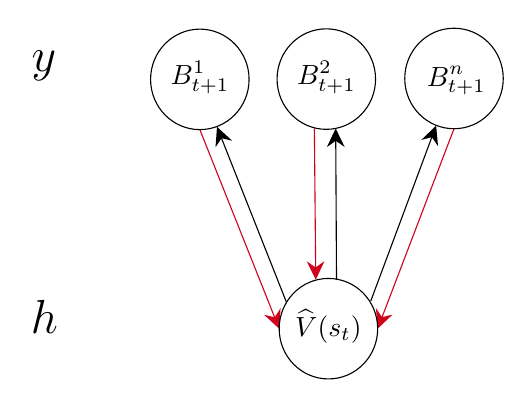
\begin{tikzpicture}[x=0.75pt,y=0.75pt,yscale=-1,xscale=1]
        %uncomment if require: \path (0,300); %set diagram left start at 0, and has height of 300
        
        %Straight Lines [id:da4267952151606098] 
        \draw    (319.82,122) -- (320.2,191.88) ;
        \draw [shift={(319.8,119)}, rotate = 89.69] [fill={rgb, 255:red, 0; green, 0; blue, 0 }  ][line width=0.08]  [draw opacity=0] (8.93,-4.29) -- (0,0) -- (8.93,4.29) -- (5.93,0) -- cycle    ;
        %Straight Lines [id:da6989378371909234] 
        \draw [color={rgb, 255:red, 208; green, 2; blue, 27 }  ,draw opacity=1 ]   (310.17,188.88) -- (309.53,119) ;
        \draw [shift={(310.2,191.88)}, rotate = 269.48] [fill={rgb, 255:red, 208; green, 2; blue, 27 }  ,fill opacity=1 ][line width=0.08]  [draw opacity=0] (8.93,-4.29) -- (0,0) -- (8.93,4.29) -- (5.93,0) -- cycle    ;
        %Shape: Ellipse [id:dp8707618719305075] 
        \draw   (353.08,94.91) .. controls (353.08,81.53) and (363.7,70.7) .. (376.81,70.7) .. controls (389.91,70.7) and (400.53,81.53) .. (400.53,94.91) .. controls (400.53,108.28) and (389.91,119.12) .. (376.81,119.12) .. controls (363.7,119.12) and (353.08,108.28) .. (353.08,94.91) -- cycle ;
        %Straight Lines [id:da13933094112344846] 
        \draw [color={rgb, 255:red, 208; green, 2; blue, 27 }  ,draw opacity=1 ]   (341.1,212.65) -- (376.81,119.12) ;
        \draw [shift={(340.03,215.46)}, rotate = 290.89] [fill={rgb, 255:red, 208; green, 2; blue, 27 }  ,fill opacity=1 ][line width=0.08]  [draw opacity=0] (8.93,-4.29) -- (0,0) -- (8.93,4.29) -- (5.93,0) -- cycle    ;
        %Shape: Ellipse [id:dp9097319337144372] 
        \draw   (291.56,95.2) .. controls (291.56,81.82) and (302.18,70.99) .. (315.29,70.99) .. controls (328.39,70.99) and (339.01,81.82) .. (339.01,95.2) .. controls (339.01,108.57) and (328.39,119.41) .. (315.29,119.41) .. controls (302.18,119.41) and (291.56,108.57) .. (291.56,95.2) -- cycle ;
        %Straight Lines [id:da3769355222150532] 
        \draw [color={rgb, 255:red, 208; green, 2; blue, 27 }  ,draw opacity=1 ]   (291.47,212.67) -- (254.35,119.55) ;
        \draw [shift={(292.58,215.46)}, rotate = 248.27] [fill={rgb, 255:red, 208; green, 2; blue, 27 }  ,fill opacity=1 ][line width=0.08]  [draw opacity=0] (8.93,-4.29) -- (0,0) -- (8.93,4.29) -- (5.93,0) -- cycle    ;
        %Straight Lines [id:da1253267073766362] 
        \draw [color={rgb, 255:red, 0; green, 0; blue, 0 }  ,draw opacity=1 ]   (263.71,120.96) -- (296.02,202.56) ;
        \draw [shift={(262.61,118.17)}, rotate = 68.4] [fill={rgb, 255:red, 0; green, 0; blue, 0 }  ,fill opacity=1 ][line width=0.08]  [draw opacity=0] (8.93,-4.29) -- (0,0) -- (8.93,4.29) -- (5.93,0) -- cycle    ;
        %Shape: Ellipse [id:dp7350394708339132] 
        \draw   (292.58,215.46) .. controls (292.58,202.09) and (303.2,191.25) .. (316.3,191.25) .. controls (329.41,191.25) and (340.03,202.09) .. (340.03,215.46) .. controls (340.03,228.83) and (329.41,239.67) .. (316.3,239.67) .. controls (303.2,239.67) and (292.58,228.83) .. (292.58,215.46) -- cycle ;
        %Shape: Ellipse [id:dp34753658855295044] 
        \draw   (230.62,95.34) .. controls (230.62,81.97) and (241.24,71.13) .. (254.35,71.13) .. controls (267.45,71.13) and (278.07,81.97) .. (278.07,95.34) .. controls (278.07,108.71) and (267.45,119.55) .. (254.35,119.55) .. controls (241.24,119.55) and (230.62,108.71) .. (230.62,95.34) -- cycle ;
        %Straight Lines [id:da6916637423351373] 
        \draw [color={rgb, 255:red, 0; green, 0; blue, 0 }  ,draw opacity=1 ]   (367.15,120.44) -- (336.7,202.13) ;
        \draw [shift={(368.2,117.63)}, rotate = 110.44] [fill={rgb, 255:red, 0; green, 0; blue, 0 }  ,fill opacity=1 ][line width=0.08]  [draw opacity=0] (8.93,-4.29) -- (0,0) -- (8.93,4.29) -- (5.93,0) -- cycle    ;
        
        % Text Node
        \draw (316.33,214.5) node   [align=left] {$\displaystyle \widehat{V}( s_{t})$};
        % Text Node
        \draw (254.43,94.4) node   [align=left] {$\displaystyle B^{1}_{t+1}$};
        % Text Node
        \draw (315.37,94.25) node   [align=left] {$\displaystyle B^{2}_{t+1}$};
        % Text Node
        \draw (377.91,95.99) node   [align=left] {$\displaystyle B^{n}_{t+1}$};
        % Text Node
        \draw (171.67,200.4) node [anchor=north west][inner sep=0.75pt]  [font=\LARGE]  {$h$};
        % Text Node
        \draw (172,80.4) node [anchor=north west][inner sep=0.75pt]  [font=\LARGE]  {$y$};
        
        \end{tikzpicture}
    \end{adjustbox}
\end{center}
\caption{\textbf{Multi-task learning in an ANN}. Adapted from \cite{bengio2017deep}. The figure represents how multi-task learning could be used in an ANN to force the the latent representation $h$ to be a sensible approximation of $V(s_t)$. Here $\widehat{V}(s_t)$ indicates the representation generated by a recurrent layer at time $t$ while $B_{t+1}=\{B^n_{t+1}: n \in N\}$ are $N$ targets quantifying the strength of the next interaction (in terms of frequency and amount of behaviour)  between $I$ and $O$. Black and red arrows are respectively the direction of the computations and the flow of the error gradient. Circles indicate computational blocks similar to those in figures \ref{fig: ffnn} and \ref{fig: ffnn_rnn}.}
\label{fig: multi_task}
\end{figure}
As we mentioned before, in order to generate a latent representation that faithfully approximate the functionality of attributed incentive salience, an ANN should be fitted simultaneously across multiple $O$. This can be achieved through what is known as a global model \cite{wang2019deep} as represented in Figure \ref{fig: global_model}.
\begin{figure}
    \begin{center}
        \begin{adjustbox}{width=0.4\textwidth}

            \tikzset{every picture/.style={line width=0.75pt}} %set default line width to 0.75pt        
            
            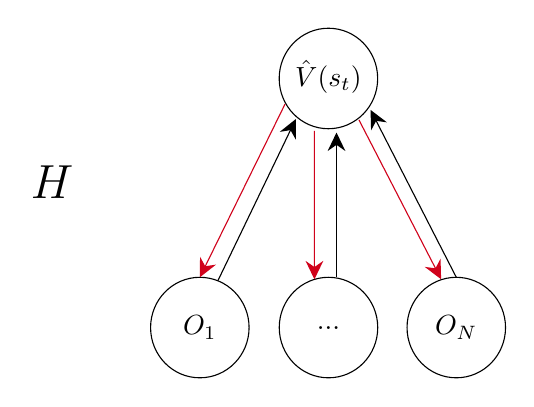
\begin{tikzpicture}[x=0.75pt,y=0.75pt,yscale=-1,xscale=1]
            %uncomment if require: \path (0,488); %set diagram left start at 0, and has height of 488
            
            %Shape: Ellipse [id:dp7350394708339132] 
            \draw   (292.58,215.46) .. controls (292.58,202.09) and (303.2,191.25) .. (316.3,191.25) .. controls (329.41,191.25) and (340.03,202.09) .. (340.03,215.46) .. controls (340.03,228.83) and (329.41,239.67) .. (316.3,239.67) .. controls (303.2,239.67) and (292.58,228.83) .. (292.58,215.46) -- cycle ;
            %Shape: Ellipse [id:dp360084071411103] 
            \draw   (230.62,335.46) .. controls (230.62,322.09) and (241.24,311.25) .. (254.35,311.25) .. controls (267.45,311.25) and (278.07,322.09) .. (278.07,335.46) .. controls (278.07,348.83) and (267.45,359.67) .. (254.35,359.67) .. controls (241.24,359.67) and (230.62,348.83) .. (230.62,335.46) -- cycle ;
            %Shape: Ellipse [id:dp6910252330291001] 
            \draw   (292.61,335.46) .. controls (292.61,322.09) and (303.23,311.25) .. (316.33,311.25) .. controls (329.44,311.25) and (340.06,322.09) .. (340.06,335.46) .. controls (340.06,348.83) and (329.44,359.67) .. (316.33,359.67) .. controls (303.23,359.67) and (292.61,348.83) .. (292.61,335.46) -- cycle ;
            %Shape: Ellipse [id:dp08711921105296772] 
            \draw   (354.18,335.46) .. controls (354.18,322.09) and (364.8,311.25) .. (377.91,311.25) .. controls (391.01,311.25) and (401.63,322.09) .. (401.63,335.46) .. controls (401.63,348.83) and (391.01,359.67) .. (377.91,359.67) .. controls (364.8,359.67) and (354.18,348.83) .. (354.18,335.46) -- cycle ;
            %Straight Lines [id:da1085527921907381] 
            \draw [color={rgb, 255:red, 208; green, 2; blue, 27 }  ,draw opacity=1 ]   (255.67,308.55) -- (295.4,227.8) ;
            \draw [shift={(254.35,311.25)}, rotate = 296.2] [fill={rgb, 255:red, 208; green, 2; blue, 27 }  ,fill opacity=1 ][line width=0.08]  [draw opacity=0] (8.93,-4.29) -- (0,0) -- (8.93,4.29) -- (5.93,0) -- cycle    ;
            %Straight Lines [id:da2379350098727664] 
            \draw [color={rgb, 255:red, 208; green, 2; blue, 27 }  ,draw opacity=1 ]   (309.56,309.25) -- (309.53,240.67) ;
            \draw [shift={(309.56,312.25)}, rotate = 269.98] [fill={rgb, 255:red, 208; green, 2; blue, 27 }  ,fill opacity=1 ][line width=0.08]  [draw opacity=0] (8.93,-4.29) -- (0,0) -- (8.93,4.29) -- (5.93,0) -- cycle    ;
            %Straight Lines [id:da04155200209198706] 
            \draw [color={rgb, 255:red, 0; green, 0; blue, 0 }  ,draw opacity=1 ]   (320.2,244.5) -- (320.2,311) ;
            \draw [shift={(320.2,241.5)}, rotate = 90] [fill={rgb, 255:red, 0; green, 0; blue, 0 }  ,fill opacity=1 ][line width=0.08]  [draw opacity=0] (8.93,-4.29) -- (0,0) -- (8.93,4.29) -- (5.93,0) -- cycle    ;
            %Straight Lines [id:da5357018140104348] 
            \draw [color={rgb, 255:red, 0; green, 0; blue, 0 }  ,draw opacity=1 ]   (299.3,237.7) -- (263,313) ;
            \draw [shift={(300.6,235)}, rotate = 115.74] [fill={rgb, 255:red, 0; green, 0; blue, 0 }  ,fill opacity=1 ][line width=0.08]  [draw opacity=0] (8.93,-4.29) -- (0,0) -- (8.93,4.29) -- (5.93,0) -- cycle    ;
            %Straight Lines [id:da1804092882370092] 
            \draw [color={rgb, 255:red, 208; green, 2; blue, 27 }  ,draw opacity=1 ]   (369.23,309.53) -- (331,235.4) ;
            \draw [shift={(370.6,312.2)}, rotate = 242.72] [fill={rgb, 255:red, 208; green, 2; blue, 27 }  ,fill opacity=1 ][line width=0.08]  [draw opacity=0] (8.93,-4.29) -- (0,0) -- (8.93,4.29) -- (5.93,0) -- cycle    ;
            %Straight Lines [id:da17854416312427956] 
            \draw [color={rgb, 255:red, 0; green, 0; blue, 0 }  ,draw opacity=1 ]   (337.97,233.27) -- (377.91,311.25) ;
            \draw [shift={(336.6,230.6)}, rotate = 62.88] [fill={rgb, 255:red, 0; green, 0; blue, 0 }  ,fill opacity=1 ][line width=0.08]  [draw opacity=0] (8.93,-4.29) -- (0,0) -- (8.93,4.29) -- (5.93,0) -- cycle    ;
            
            % Text Node
            \draw (316.33,214.5) node   [align=left] {$\displaystyle \hat{V}( s_{t})$};
            % Text Node
            \draw (171.67,256.4) node [anchor=north west][inner sep=0.75pt]  [font=\LARGE]  {$H$};
            % Text Node
            \draw (254.35,335.46) node   [align=left] {$\displaystyle O_{1}$};
            % Text Node
            \draw (316.33,335.46) node   [align=left] {$\displaystyle ...$};
            % Text Node
            \draw (377.91,335.46) node   [align=left] {$\displaystyle O_{N}$};
            \end{tikzpicture}
        \end{adjustbox}
    \end{center}
\caption[\textbf{Diagram of a Global Model}]{The figure represents how multiple $O$ can simultaneously contribute to the estimation of $\widehat{V}(s_t)$. Here $\{O_1, \dots, O_N\}$ indicate a set of object on which the ANN is simultaneously fit. Black and red arrows are respectively the direction of the computations and the flow of the error gradient. Circles indicate computational blocks similar to those in figures \ref{fig: ffnn} and \ref{fig: ffnn_rnn}.}
\label{fig: global_model}
\end{figure}
These models can be thought as an extension of mixed effects models \cite{crawley2007mixed} to ANNs and assume that the data on which the model is fitted are drawn from a hierarchy of different populations, each one with its own heterogeneity which can however be brought back to a common single latent factor. The concept is similar to that of Bayesian hierarchical models \cite{gelman2020bayesian} and has the effect of allowing information sharing across the different levels of the hierarchy while also promoting regularization (and therefore generalization)\cite{gelman2020bayesian}. The underlying mechanisms is known as partial pooling \cite{gelman2020bayesian} and can be seen as a middle ground between the over-generalizability of complete pooling (where a single model is estimated across all the levels of the hierarchy) and the over-specificity of un-pooling (where multiple models are estimated, one for each level of the hierarchy). As we can see from Figure \ref{fig: global_model} all the different $O$ contribute to the estimation of a single latent representation $V(s_t)$ which also provide the error gradient for updating their associated parameters.

\subsection{Modelling the contribution of Game Events and Environment Indicators}
\label{modelling_env_and_game_elements}
As we mentioned in chapter \ref{chapter_lit_review}, the current ammount of attributed incentive salience is in part conditioned by the characteristics of the game while its behavioural manifestation can be affected by the environment surrounding the individual. These two factors are not taken into consideration in the modelling framework we just proposed, indeed we assume them to be absorbed, to a certain extent, by the behavioural indicator $B$. If the game characteristics are not able to provide sufficient rewarding experiences or some environmental factors act as an impediment, we can expect to observe less intense and frequent interactions between $I$ and $O$. However in this setting it would be hard to disentangle which factors contributed to the reduction in observed behaviour: was it due to a long-running decline in the level of attributed incentive salience or to an unfavourable conjunction of in-game and out-game events? In this view introducing historical information about the interaction than an individual had with particular characterisitcs of the game object and the environmental context in which they occurred should not just improve the prediction of $\widehat{B}_{t+1}$ but also the estimation of $\widehat{V}(s_t)$. Of course introducing and modelling an extra set of predictors in an ANN is relatively straightforward and increasing the number of available parameters should help incorporating the additional information, however this would make the interpretation of the derived latent representation even more challenging. A possible solution to this problem is to modify the architecture of the ANN in order to integrate the addtional information in a similar way to what Generalized Additive Model (GAM) would do \cite{hastie2017generalized}. Solving the problem of predicting $B_{t+1}$ within a GAM framework for a single game object could have the following formulation:
\begin{gather}
\label{gam}
    \widehat{B}_{t+1} = \beta + f^{B}(B_{t:t-n};\theta^{B}) + f^{G}(G_{t:t-n};\theta^{G}) + f^{Env}(Env_{t:t-n};\theta^{Env})
\end{gather}
here $\beta$ is a generic intercept while $B_{t:t-n}$, $G_{t:t-n}$ and $Env_{t:t-n}$ are temporal series of behavioural metrics, game events and environment indicators up to time $t$. The corresponding functions $f^{B}$, $f^{G}$ and $f^{Env}$ are usually linear or non linear (e.g. splines) additive models. The framework offered by GAM is a good compromise between complexity and explainability as it allows to consider many predictors while enforcing a structural form that makes the function associated to each of them directly interpretable \cite{hastie2017generalized}. In a work by Agarwal et al. \cite{agarwal2021neural} the authors extended the GAM framework to ANN (Neural Addtive Models, NAM), the general idea behind this is to substitute each function expressed in equation \ref{gam} with an appropriated ANN and to derive the prediction of the model as a linear combination of them. The additive nature of NAM, despite posing a constrain on how each function gets integrated with the others, makes it possible to know exactly how each function contribute to the final prediction \cite{hastie2017generalized,agarwal2017quitting}. In our setting we are less interested in retrieving the exact functional form associated to any of the three sources of information (i.e. behaviour, game characteristics and environment) and more in being able to generate separable representations for each one of them. In this view, combining the functional form of equation \ref{gam} with the ideas presented in this chapter we could formulate the estimation of $V(s_t)$ as a non-linear combination of separate functions (all parametrized by ANNs) and subsequently use this for predicting $B_{t+1}$
\begin{gather}
\label{nam}
    \widehat{B_t} = f^{B}(B_{t:t-n}, O;\theta^{B}) \\
    \widehat{G_t} = f^{G}(G_{t:t-n}, O;\theta^{G}) \\ 
    \widehat{Env_t} = f^{Env}(Env_{t:t-n}, O;\theta^{Env}) \\
    \widehat{V}(s_t) = f^{V}(B_t, G_t, Env_t; \theta^{V}) \nonumber
\end{gather}
here $\widehat{B_t}$, $\widehat{G_t}$, $\widehat{Env_t}$ and $\widehat{V}(s_t)$ are representation generated by the respective functions $f$. Each function can be though as being parametrized by a recurrent ANN as specified in section \ref{rnn_theory}. The final representation $\widehat{V}(s_t)$ would then be used for solving the same type of multi-task learning problem presented in section \ref{manifold_learning}. A graphic representation for this can be found in figure \ref{fig: nam_multi_task}.
\begin{figure}
    \begin{center}
        \begin{adjustbox}{width=0.4\textwidth}

            \tikzset{every picture/.style={line width=0.75pt}} %set default line width to 0.75pt        
            
            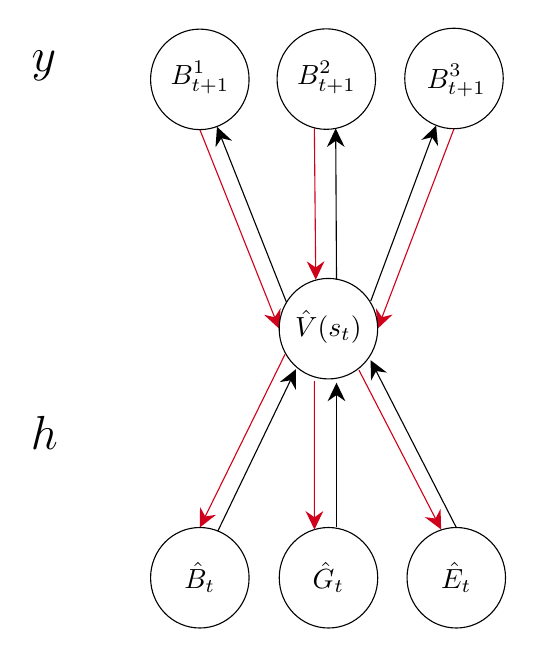
\begin{tikzpicture}[x=0.75pt,y=0.75pt,yscale=-1,xscale=1]
            %uncomment if require: \path (0,488); %set diagram left start at 0, and has height of 488
            
            %Straight Lines [id:da4267952151606098] 
            \draw    (319.82,122) -- (320.2,191.88) ;
            \draw [shift={(319.8,119)}, rotate = 89.69] [fill={rgb, 255:red, 0; green, 0; blue, 0 }  ][line width=0.08]  [draw opacity=0] (8.93,-4.29) -- (0,0) -- (8.93,4.29) -- (5.93,0) -- cycle    ;
            %Straight Lines [id:da6989378371909234] 
            \draw [color={rgb, 255:red, 208; green, 2; blue, 27 }  ,draw opacity=1 ]   (310.17,188.88) -- (309.53,119) ;
            \draw [shift={(310.2,191.88)}, rotate = 269.48] [fill={rgb, 255:red, 208; green, 2; blue, 27 }  ,fill opacity=1 ][line width=0.08]  [draw opacity=0] (8.93,-4.29) -- (0,0) -- (8.93,4.29) -- (5.93,0) -- cycle    ;
            %Shape: Ellipse [id:dp8707618719305075] 
            \draw   (353.08,94.91) .. controls (353.08,81.53) and (363.7,70.7) .. (376.81,70.7) .. controls (389.91,70.7) and (400.53,81.53) .. (400.53,94.91) .. controls (400.53,108.28) and (389.91,119.12) .. (376.81,119.12) .. controls (363.7,119.12) and (353.08,108.28) .. (353.08,94.91) -- cycle ;
            %Straight Lines [id:da13933094112344846] 
            \draw [color={rgb, 255:red, 208; green, 2; blue, 27 }  ,draw opacity=1 ]   (341.1,212.65) -- (376.81,119.12) ;
            \draw [shift={(340.03,215.46)}, rotate = 290.89] [fill={rgb, 255:red, 208; green, 2; blue, 27 }  ,fill opacity=1 ][line width=0.08]  [draw opacity=0] (8.93,-4.29) -- (0,0) -- (8.93,4.29) -- (5.93,0) -- cycle    ;
            %Shape: Ellipse [id:dp9097319337144372] 
            \draw   (291.56,95.2) .. controls (291.56,81.82) and (302.18,70.99) .. (315.29,70.99) .. controls (328.39,70.99) and (339.01,81.82) .. (339.01,95.2) .. controls (339.01,108.57) and (328.39,119.41) .. (315.29,119.41) .. controls (302.18,119.41) and (291.56,108.57) .. (291.56,95.2) -- cycle ;
            %Straight Lines [id:da3769355222150532] 
            \draw [color={rgb, 255:red, 208; green, 2; blue, 27 }  ,draw opacity=1 ]   (291.47,212.67) -- (254.35,119.55) ;
            \draw [shift={(292.58,215.46)}, rotate = 248.27] [fill={rgb, 255:red, 208; green, 2; blue, 27 }  ,fill opacity=1 ][line width=0.08]  [draw opacity=0] (8.93,-4.29) -- (0,0) -- (8.93,4.29) -- (5.93,0) -- cycle    ;
            %Straight Lines [id:da1253267073766362] 
            \draw [color={rgb, 255:red, 0; green, 0; blue, 0 }  ,draw opacity=1 ]   (263.71,120.96) -- (296.02,202.56) ;
            \draw [shift={(262.61,118.17)}, rotate = 68.4] [fill={rgb, 255:red, 0; green, 0; blue, 0 }  ,fill opacity=1 ][line width=0.08]  [draw opacity=0] (8.93,-4.29) -- (0,0) -- (8.93,4.29) -- (5.93,0) -- cycle    ;
            %Shape: Ellipse [id:dp7350394708339132] 
            \draw   (292.58,215.46) .. controls (292.58,202.09) and (303.2,191.25) .. (316.3,191.25) .. controls (329.41,191.25) and (340.03,202.09) .. (340.03,215.46) .. controls (340.03,228.83) and (329.41,239.67) .. (316.3,239.67) .. controls (303.2,239.67) and (292.58,228.83) .. (292.58,215.46) -- cycle ;
            %Shape: Ellipse [id:dp34753658855295044] 
            \draw   (230.62,95.34) .. controls (230.62,81.97) and (241.24,71.13) .. (254.35,71.13) .. controls (267.45,71.13) and (278.07,81.97) .. (278.07,95.34) .. controls (278.07,108.71) and (267.45,119.55) .. (254.35,119.55) .. controls (241.24,119.55) and (230.62,108.71) .. (230.62,95.34) -- cycle ;
            %Straight Lines [id:da6916637423351373] 
            \draw [color={rgb, 255:red, 0; green, 0; blue, 0 }  ,draw opacity=1 ]   (367.15,120.44) -- (336.7,202.13) ;
            \draw [shift={(368.2,117.63)}, rotate = 110.44] [fill={rgb, 255:red, 0; green, 0; blue, 0 }  ,fill opacity=1 ][line width=0.08]  [draw opacity=0] (8.93,-4.29) -- (0,0) -- (8.93,4.29) -- (5.93,0) -- cycle    ;
            %Shape: Ellipse [id:dp360084071411103] 
            \draw   (230.62,335.46) .. controls (230.62,322.09) and (241.24,311.25) .. (254.35,311.25) .. controls (267.45,311.25) and (278.07,322.09) .. (278.07,335.46) .. controls (278.07,348.83) and (267.45,359.67) .. (254.35,359.67) .. controls (241.24,359.67) and (230.62,348.83) .. (230.62,335.46) -- cycle ;
            %Shape: Ellipse [id:dp6910252330291001] 
            \draw   (292.61,335.46) .. controls (292.61,322.09) and (303.23,311.25) .. (316.33,311.25) .. controls (329.44,311.25) and (340.06,322.09) .. (340.06,335.46) .. controls (340.06,348.83) and (329.44,359.67) .. (316.33,359.67) .. controls (303.23,359.67) and (292.61,348.83) .. (292.61,335.46) -- cycle ;
            %Shape: Ellipse [id:dp08711921105296772] 
            \draw   (354.18,335.46) .. controls (354.18,322.09) and (364.8,311.25) .. (377.91,311.25) .. controls (391.01,311.25) and (401.63,322.09) .. (401.63,335.46) .. controls (401.63,348.83) and (391.01,359.67) .. (377.91,359.67) .. controls (364.8,359.67) and (354.18,348.83) .. (354.18,335.46) -- cycle ;
            %Straight Lines [id:da1085527921907381] 
            \draw [color={rgb, 255:red, 208; green, 2; blue, 27 }  ,draw opacity=1 ]   (255.67,308.55) -- (295.4,227.8) ;
            \draw [shift={(254.35,311.25)}, rotate = 296.2] [fill={rgb, 255:red, 208; green, 2; blue, 27 }  ,fill opacity=1 ][line width=0.08]  [draw opacity=0] (8.93,-4.29) -- (0,0) -- (8.93,4.29) -- (5.93,0) -- cycle    ;
            %Straight Lines [id:da2379350098727664] 
            \draw [color={rgb, 255:red, 208; green, 2; blue, 27 }  ,draw opacity=1 ]   (309.56,309.25) -- (309.53,240.67) ;
            \draw [shift={(309.56,312.25)}, rotate = 269.98] [fill={rgb, 255:red, 208; green, 2; blue, 27 }  ,fill opacity=1 ][line width=0.08]  [draw opacity=0] (8.93,-4.29) -- (0,0) -- (8.93,4.29) -- (5.93,0) -- cycle    ;
            %Straight Lines [id:da04155200209198706] 
            \draw [color={rgb, 255:red, 0; green, 0; blue, 0 }  ,draw opacity=1 ]   (320.2,244.5) -- (320.2,311) ;
            \draw [shift={(320.2,241.5)}, rotate = 90] [fill={rgb, 255:red, 0; green, 0; blue, 0 }  ,fill opacity=1 ][line width=0.08]  [draw opacity=0] (8.93,-4.29) -- (0,0) -- (8.93,4.29) -- (5.93,0) -- cycle    ;
            %Straight Lines [id:da5357018140104348] 
            \draw [color={rgb, 255:red, 0; green, 0; blue, 0 }  ,draw opacity=1 ]   (299.3,237.7) -- (263,313) ;
            \draw [shift={(300.6,235)}, rotate = 115.74] [fill={rgb, 255:red, 0; green, 0; blue, 0 }  ,fill opacity=1 ][line width=0.08]  [draw opacity=0] (8.93,-4.29) -- (0,0) -- (8.93,4.29) -- (5.93,0) -- cycle    ;
            %Straight Lines [id:da1804092882370092] 
            \draw [color={rgb, 255:red, 208; green, 2; blue, 27 }  ,draw opacity=1 ]   (369.23,309.53) -- (331,235.4) ;
            \draw [shift={(370.6,312.2)}, rotate = 242.72] [fill={rgb, 255:red, 208; green, 2; blue, 27 }  ,fill opacity=1 ][line width=0.08]  [draw opacity=0] (8.93,-4.29) -- (0,0) -- (8.93,4.29) -- (5.93,0) -- cycle    ;
            %Straight Lines [id:da17854416312427956] 
            \draw [color={rgb, 255:red, 0; green, 0; blue, 0 }  ,draw opacity=1 ]   (337.97,233.27) -- (377.91,311.25) ;
            \draw [shift={(336.6,230.6)}, rotate = 62.88] [fill={rgb, 255:red, 0; green, 0; blue, 0 }  ,fill opacity=1 ][line width=0.08]  [draw opacity=0] (8.93,-4.29) -- (0,0) -- (8.93,4.29) -- (5.93,0) -- cycle    ;
            
            % Text Node
            \draw (316.33,214.5) node   [align=left] {$\displaystyle \hat{V}( s_{t})$};
            % Text Node
            \draw (254.43,94.4) node   [align=left] {$\displaystyle B_{t+1}^{1}$};
            % Text Node
            \draw (315.37,94.25) node   [align=left] {$\displaystyle B_{t+1}^{2}$};
            % Text Node
            \draw (377.91,95.99) node   [align=left] {$\displaystyle B_{t+1}^{3}$};
            % Text Node
            \draw (171.67,256.4) node [anchor=north west][inner sep=0.75pt]  [font=\LARGE]  {$h$};
            % Text Node
            \draw (172,80.4) node [anchor=north west][inner sep=0.75pt]  [font=\LARGE]  {$y$};
            % Text Node
            \draw (254.35,335.46) node   [align=left] {$\displaystyle \hat{B}_{t}$};
            % Text Node
            \draw (316.33,335.46) node   [align=left] {$\displaystyle \hat{G}_{t}$};
            % Text Node
            \draw (377.91,335.46) node   [align=left] {$\displaystyle \hat{E}_{t}$};
            \end{tikzpicture}
        \end{adjustbox}
    \end{center}
\caption{\textbf{Multi-task learning with factorization}. Adapted from \cite{bengio2017deep}. The figure represents how multi-task learning could be extended for distinctly modelling the contribution of different factors in the estimation of $\widehat{V}(s_t)$. Here $\widehat{B_t}$, $\widehat{G_t}$ and $\widehat{E_t}$ indicate the representations generated by 3 distinct recurrent layers taking as input: behavioural, game-events and environmental indicators. The three representations are then parsed by a subsequent recurrent layer producing $\widehat{V}(s_t)$. Similarly to figure \ref{fig: multi_task}, $B_{t+1}=\{B^n_{t+1}: n \in N\}$ are $N$ targets quantifying the strength of the next interaction (in terms of frequency and amount of behaviour)  between $I$ and $O$. Black and red arrows are respectively the direction of the computations and the flow of the error gradient. Circles indicate computational blocks similar to those in figures \ref{fig: ffnn} and \ref{fig: ffnn_rnn}.}
\label{fig: fact_multi_task}
\end{figure}

\section{Discussion}
In this chapter we introduced the idea that latent states, like attributed incentive salience, despite being encoded by high-dimensional signals (e.g. patterns of brain or behavioural activities), can be effectively approximated by a lower dimensional manifold \cite{gallego2017neural, derdikman2011manifold, nieh2021geometry, bromberg2010coding, seung2000manifold, ganmor2015thesaurus, stopfer2003intensity}. We then specified how in the literature the modelling and estimation of attributed incentive salience was carried out through reinforcement learning (i.e. TD learning) \cite{mcclure2003computational,zhang2009neural}. This approach allows to specify the dynamics underlying the process of saliency attribution and offers a direct interpretation of the estimated representations. However, its application in complex naturalistic scenarios can be challenging. Leveraging the knowledge presented in chapter \ref{chapter_lit_review} in combination with insights derived by previous computational model of attributed incentive salience \cite{mcclure2003computational,zhang2009neural} we proposed to approximate the ammount of attributed incentive salience through supervised learning. Due to their reliance on reward mechanics and the ability to provide large volumes of ecologically sound data we thought videogames to be the optimal test bed for our methodology. For this purpose we designed an ANN able to incorporate information about the state of the individual, the environment surrounding them and their interaction with the game. We argued that ANNs with recurrent operations would be well suited for the task as they generate latent representations through dynamical mechanisms that are similar to those of TD learning \cite{barto2004reinforcement}. We also stressed the necessity to learn a single model able to simultaneously incorporate information across multiple videogames in order to obtain representations that obey to the same functional constrains of motivation that we specified in chapter \ref{chapter_lit_review}: namely the ability to simultaneously describe the propensity towards multiple rewarding objects. In the next chapter we will proceeded at illustrating the implementation of the computational model presented in this chapter and the experimental validation of its underlying assumptions.

\chapter{Model Implementation and Testing}
\label{chapter_implementation_testing}
\section{Introduction}
\label{implementation_testing_introduction}

In this chapter we will outline the implementation of the model described in chapter 2. We adopted a variation of bottom-up iterative model building process in which first the simplest version of a model is designed, built and tested and then, based on the perfromance of this model and addition theoretical assumption a new improved version of the same model is designed. At each stage of the model building process we test the new version of the model against alternative approaches in order to test for specific hypothesis stated in the model design stage. Each section of this chapter corresponds to a different version of the model and will have the following structure. In Model design we state the task the model is trying to solve, the design of such model and the theoretical assumptions that informed the design. In data we describe the dataset used for evaluating the perfromance of our model along with any data-related processing. In model Comparison Procedure we outline the alternative models against which our model is compared and the procedure adopted for the comparison. In results we describe the outcome of the model comparison procedure. In model criticism we discuss the results in light of the theoretical assumptions stated in Model Design and highlight potential improvements of the model design.

\section{Joint Prediction of Future Behavioural Intensity}
\label{model_architecture_1}

\subsection{Model Design}
We present a novel deep neural network architecture, loosely inspired by the winning entry in \cite{lee2018game}, for jointly estimate survival time and churn probability. This architecture, the `Bifurcating Model' (BM), is demonstrated in Fig. \ref{bm_architecture}. The model receives, as input, both a vector of unfolded features, as in Table \ref{metricsdescription}, as well as a context vector containing a numerical encoding of the game (e.g. jc3 = $[1]$, lis = $[2]$ etc.). The game context is then embedded into a vector of $l = 40$, similarly to what is done in words embedding for sentiment analysis \cite{chollet2015keras}. Differently from a one-hot encoding, this approach provides a non-sparse representation of the input while also projecting it into a multi-dimensional space where the relationships between elements become meaningful (e.g. game contexts which are similar to each other in respect to the objectives will be located closer to each other in the embedding space). Using an embedding for encoding the game contexts allows to have a representation that grows richer and richer the more categories are included into it. Obviously this would require to re-train the model whenever a new unseen context is added, practice however not just advisable but also routinely done in production. Next, the raw behavioural input and the embedded game context vector are concatenated along the temporal dimension into a single feature vector and a zero-padding re-applied where needed. At this point, a masking layer allows the model to more efficiently work with time-series of different lengths (i.e. skipping the computations for the zero-padded time-steps) and a dense layer, applied to each time step, to combine raw behavioural metrics and context in a new vector of $l = 40$. These newly obtained features are then modelled across time using a Long Short-Term Memory (LSTM) recurrent layer with $n = 100$ units. Therefore, the output of this LSTM Layer is a feature vector of $l = 100$ which is a latent representation of the input features across time and can be seen as providing a high-level representation of the behavioural state of the user during the OP. The final step of this architecture is to then take this high-level latent representation and pass it to a pair of shallow NNs, one tasked with estimating survival time and the other churn probability. These estimators are formed of a pair of densely connected layers, where the first layer has $n = 300$ units and the last has $n = 1$ units, the output of which will constitute the survival time and churn probability estimates. Like the two MLP models the BM was batch trained with a batch size of 256 until convergence using the ADAM optimizer, with learning rate adjusted through a cyclical policy \cite{smith2017cyclical, chollet2015keras}, minimizing the sum of the two losses. Similarly to the MLP models, the hidden layers used $ReLU$ as activation function whereas the two outputs units used respectively an $identity$ and $sigmoid$ functions for producing the survival time and churn probability estimates. For the survival time branch SMAPE was used as an objective function while for the churn estimation branch BCE was adopted. We applied two regularization techniques after the computations of the first layers of each shallow NN, batch normalization \cite{ioffe2015batch} and dropout \cite{srivastava2014dropout} ($rate = 0.1$). Additionally, following the intuition from \cite{gal2016dropout}, we employed dropout also at inference time for sampling from the model parameters and obtaining a distribution over the posterior so to be able to represent uncertainty in the model estimates. This was achieved by querying the model 50 times at prediction time and retaining all the produced values. When computing the performance metrics we then used the mean of the estimated values, since they roughly followed a normal distribution the mean could be seen as the value with highest probability. All the experiments were implemented in Python 3.6, with the algorithms for Experiment 1 and 2 provided by the library scikit-learn \cite{scikit-learn} and our novel BM architecture developed using Keras with Tensorflow as a back-end \cite{chollet2015keras}.

\subsection{Data}
To conduct our experiments, we gathered data from six different games published by our partner company, \textit{Square Enix Limited}. Focusing on maintaining heterogeneity in genre and platform, we considered the following titles: \emph{Hitman Go} (hmg), \emph{Hitman Sniper} (hms), \emph{Just Cause 3} (jc3), \emph{Just Cause 4} (jc4), \emph{Life is Strange} (lis), and \emph{Life is Strange: Before the Storm} (lisbf). A general description of each of these titles can be found in Table \ref{gamesdescription}. Data were gathered from any user playing between the game's release and February 2019, allowing us to adopt more robust sampling strategies which utilizes the breadth of virtually the entire user-base. To rule out possible `faulty' but not `naturally abnormal' data, we restricted the data cleaning process to a single filter applied at query time to ignore users having at least one of the considered metric over the game population's \nth{99} percentile. This allowed us to make little assumptions on the distribution of the data as well as providing a convenient stress test for eventual future applications.

\begin{table}[h] 
\centering
\caption[\textbf{Data-set Description}]{For each game we retrieved 80,000 Churners and 80,000 Non-Churners randomly sampled from all the available users.}
\label{game_description_31}
\begin{tabularx}{\textwidth}{@{}lrrrrrrX@{}}
\toprule

\multirow{2}{*}{\textbf{Game}} & \multicolumn{2}{l}{\textbf{Survival Time (Mins})} & \multirow{2}{*}{\textbf{Churners}} & \multirow{2}{*}{\textbf{Non Churners}} & \multicolumn{2}{l}{\textbf{Observation Period}} & \multirow{2}{*}{\textbf{Type}} \\ \cmidrule(lr){2-3} \cmidrule(lr){6-7}
                      & \textbf{Min}                  & \textbf{Max}                  &                           &                               & \textbf{Min}                & \textbf{Max}               &                                \\ \midrule
hmg                        & 11 & 260    & 80,000 & 80,000  & 1  & 7  & Mobile Strategy                       \\
hms                        & 2 & 454     & 80,000 & 80,000  & 1  & 15 & Mobile Shooting Gallery                \\
jc3                        & 32 & 12,695 & 80,000 & 80,000  & 1  & 20 & Console Action Open World             \\
jc4                        & 7 & 1,135   & 80,000 & 80,000  & 1  & 9  & Console Action Open World           \\
lis                        & 5 & 704     & 80,000 & 80,000  & 1  & 6  & Console Graphic Adventure \\
libf                       & 14 & 1,214  & 80,000 & 80,000  & 1  & 10 &  Console Graphic Adventure \\ \bottomrule
\end{tabularx}
\end{table}

\paragraph*{Defining the Observation Period}
Because we were interested in estimating survival time and churn probability based only on early user-game interactions it was important to define a cut-off at which point interactions were no longer be considered `early'. We call the period from the user's first interaction till this cut-off the observation period (OP). Choosing the length for the OP was not trivial as there is little indication in the literature about optimal cut-off values. Hence, we decided to visually inspect the data a-priori and extend rules proposed in \cite{drachen2016rapid, milovsevic2017early} to take into account natural inter-individual differences. Therefore, we defined the cut-off as:

\begin{equation}
\label{CutoffOP}
    \text{cutoff} = 
    \Biggl\lceil
        \dfrac
            {min(S_t, S_c)}
            {3}
    \Biggr\rceil
\end{equation}

Where $S_t$ is the total number of game play sessions and $S_c$ is the number of game play sessions before the user completed the game for the first time. In this way we take the first \sfrac{1}{3} of all played sessions for players who churned and the first \sfrac{1}{3} of played sessions before a non-churning player completed the game for the first time. We apply this cut off to the ordered list of all recorded play sessions for a specific user. We decided to use game sessions as the temporal dimension, rather than total minutes played, since we believed it better adjusted for each user's `pace' (i.e. not all the users have the possibility to play at the same frequency). Since the length of the OP has a naturally different distribution between the churning and non-churning population, we stratified our sampling technique to maintain a similar ratio of OP lengths among churners and non churners. This becomes particularly relevant for Experiment 2 and 3 where the length of the OP could leak information in the churn probability estimation task. Summarizing, if a user for example had 9 total sessions recorded, we considered the first 3 for making estimations on what happened after the 9$^{th}$. It goes without saying that at production time the OP is defined only for generating the training samples, the model can be deployed at various stages of previously unseen time series which we simulate in our experiments with the test set. 

\paragraph*{Defining the Behavioural Metrics and Targets}
We considered a set of 5 metrics, easily generalizable across games and indicative of behavioural activity, and retrieved them temporally  (i.e. over each game session during the OP), see Table \ref{metricsdescription} for a description. Additionally, we acquired a single context feature specifying the game context from where the metrics were originated. For determining the targets for our survival and churn estimation tasks, we leveraged existing literature on churn prediction \cite{drachen2016rapid, milovsevic2017early, lee2018game, perianez2016churn, runge2014churn, kim2017churn, hadiji2014predicting, xie2015predicting} and survival analysis \cite{viljanen2018playtime, demediuk2018player, lee2018game, bertens2017games}, extending existing rules to accommodate the need to define churn and survival time in single player games with a defined life cycle (i.e. non-GaaS games). We took advantage of having access to the complete session history for all users to create a churn definition which was robust to the variance in play patterns across games, as it takes into account all the recorded inter-session distances. Therefore, the criteria we adopted for defining a user as churner were both: 

\begin{enumerate}
    \item Not completing the game
    \item Being inactive for a period equal or greater to:
        \begin{equation}
            \label{inactivityrule}
            \text{inactivity} = 
            mean(\mathbf{x}) + 2.5 \cdot std(\mathbf{x})
        \end{equation}
\end{enumerate}

For better adjusting for inter-individual differences, we could have applied formula \ref{inactivityrule} to each user individually but this could have created accuracy issue for individuals with very few recorded sessions. Therefore, we opted for a conservative but more robust approach applying inactivity ($\mathbf{x}$) $\forall \mathbf{x} \in X$ where $X$ is the collection of all the considered games and $\mathbf{x}$ is the vector of inter-sessions distances in minutes for a specific game. The use of formula \ref{inactivityrule} allowed us to estimate an inactivity period which was not arbitrarily chosen but statistically defined as ‘extraordinary long’ in accordance with characteristics of play patterns in a particular game. For defining the survival time, we simply computed the total amount of Play Time in minutes for a user minus the amount of Play Time during the OP.

\begin{table}[h] \centering
\caption{\textbf{Considered Metrics over Sessions}}
\label{metricsdescription}
\resizebox{0.5\textwidth}{!}{
\begin{tabular}{@{}ll@{}}
\toprule
\textbf{Metric}            & \textbf{Description}                   \\ \midrule
{Session Time}         & Overall session duration (minutes)              \\ 
{Play Time}            & Session Time spent actively playing (minutes)    \\ 
{Delta Session}        & Temporal distance  between sessions (minutes)   \\ 
{Activity Index}       & Count of user initiated game-play-related actions. E.g.\\ 
                       & `Talk to NPC' or `Acquire Upgrade' were considered valid\\ 
                       & actions while `Click Menu' or `NPC Attacks You' were not.\\
{Activity Diversity}   & Count of unique voluntarily initiated actions \\ 
{Context}              & Name of the game taken into consideration \\ \bottomrule
\end{tabular}
}
\end{table}

\paragraph*{Data Preparation}We adopted specific data preparation procedures for each experiment. For the first analysis we collapsed the data over the temporal dimension retrieving mean and standard deviation of each considered features, to this concatenating a one-hot encoded transformation of the context metric. For the second and third experiments we kept the data in the original temporal form. In Experiment 3 only we treated the game context slightly differently, numerically encoding it and separating it from the other feature matrix. Since in Experiment 2 and 3 the length of the OP differed between users, we zero padded each sequence of considered sessions to the length of the longest sequence in the data-set. For each experiment we created a tuning and validation subsets (i.e. 20 and 80 \% of the original data-set) via stratified shuffle split \cite{scikit-learn}, employing the first for hyper-parameters searching and the second for model evaluation.

\subsection{Model Comparison}
For all experiments we applied the same procedure: first, determined the best hyper-parameters via grid search 10-fold stratified cross validation \cite{scikit-learn} on the tuning set then evaluated performance via 10-fold stratified cross validation on the validation set. In all experiments, we re-scaled the considered metric separately for each game in outliers-robust way, as in:

\begin{equation}
\label{robustscaler}
    \text{RobustRescale}=
        \dfrac
            {\mathbf{x} - Q_2(\mathbf{x})}
            {Q_3(\mathbf{x}) - Q_1(\mathbf{x})}
\end{equation}

where $\mathbf{x}$ is the feature vector to be re-scaled and $Q_n$ is the $n^{th}$ quartile for this game. The performance metric that we chose for our survival task was the Symmetric Mean Absolute Percentage Error (SMAPE), defined as:



where $N$ is the collection of all the users in the considered set and $\hat{y_i}$ and $y_i$ are respectively estimated survival time and ground truth value for user \textit{i}. SMAPE was implemented because its scale invariance allowed better comparisons of results across game contexts. For the churn estimation task the chosen metric was the F1 score (F1), defined as:

\begin{equation}
\label{f1}
    \text{F1}=
        2 \cdot 
        \dfrac
            {(precision \cdot recall)}
            {(precision + recall)}
\end{equation}

with $precision =\frac {TP}{(TP + FP)}$ and $recall = \frac {TP}{(TP + FN)}$, where \textit{TP, FP, TN, FN} stand for True Positives, False Positives, True Negatives and False Negatives. We chose the macro-averaged F1 (i.e. employing the unweighted mean of precision and recall for both classes) since our data-set was perfectly balanced.

\paragraph*{Competing Models}
As well as our novel model for joint survival time and churn probability estimation we discuss several models for disjoint estimation, learning only survival time or churn probability, in order to conduct our experiments and  compare our model with existing techniques. Furthermore, for providing a baseline comparison in our experiments we employed a mean model (MM), which generates predictions based on the average of the targets in the training set. The choice of disjoint estimation models was dictated by a series of needs: widespread usage in research and industry settings, ability to capture linear and non-linear interactions between features and most importantly capability to train on large data-sets (e.g. matrix of dimension $\approx10^6\times10^2$). Four models were employed in Experiments 1 and 2. Firstly, a variant of Regularized Regression, ElasticNet (EN) \cite{zou2005regularization}, for survival estimation and Logistic Regression (LR) for churn probability estimation. Secondly, a pair of similar Multi-Layers Perceptron Neural Networks, one tasked to perform survival time regression, MLPr, and one to perform churn classification, MLPc. We felt that given the similarities between linear models and NNs, which can be seen as a stacked version of the former with more `expressive power', the chosen algorithms constituted a natural progression in the modelling approach. For EN the best hyper-parameters were $\alpha = 0.1$ and a ratio of $0.5$ between l1 and l2 regularization. For LR an l1 regularization with $C = 0.01$. Both MLPr and MLPc employed an l2 penalty of $0.01$ and utilized a 3 layers architecture with 200, 100 and 50 hidden units. For all hidden units a $ReLU(z) = max(0, z)$ activation function was used, while an  $identity(z) = z$ and $ sigmoid(z) = \frac {1} {1 + \epsilon^{-z}}$ functions were respectively used as final activations for the MLPr and MLPc, where $z$ is a weighted sum of the hidden units of the previous layer. When training the MLP based models a small sub-set was extracted from the training set which represented 10\% of the data. This sub-set was used to evaluate convergence of the model and stop the training phase before over-fitting could occur. For both models convergence was determined if the loss did not improve for 3 epochs. The networks were trained using a batch size of 256 and optimized using the Adaptive Moment Estimation (ADAM) optimizer \cite{kingma2014adam}. Because survival time estimation is a regression task and churn prediction is classification task different loss function were used, Mean Squared Error (MSE) and Binary Cross Entropy (BCE) respectively. These are defined as:

\begin{equation}
\label{mae}
    \text{MSE}=
        \dfrac
            {1}
            {N}
            \sum\limits_{i=1}^{N}  (y_i - \hat{y_i})^2
\end{equation}
\begin{equation}
\label{bce}
    \text{BCE}=
        -\dfrac
            {1}
            {N}
        \sum\limits_{i=1}^{N}  y_i \cdot log(\hat{y_i}) + (1-y_i) \cdot log(1 - \hat{y_i})
\end{equation}

where $N$ is the size of the batch, and $\hat{y_i}$ and $y_i$ are respectively estimations provided by the model and ground truth value for the $i_{th}$ element in the batch. 

\subsection{Results}
We will first present results for each disjoint model as well as for a baseline model. Next we will illustrate in detail the performance of the BM model both in terms of it's raw accuracy as well as its capability to include uncertainty in it's output. Note that for all reported SMAPE results the smaller the better as it represents the error between the prediction and ground truth. Conversely, for F1 the larger the better since it measures how often the trained model made the correct classifications without false alarms. The probability threshold employed for discriminating between classes was set to 0.5.
\begin{table}[h]\centering
\caption{\textbf{Performance Baseline Mean Model}}
\label{baseperformance}
\resizebox{0.5\textwidth}{!}{
\begin{tabular}{@{}llrr@{}}
\toprule
\textbf{Game}  &\textbf{Model}                 & \textbf{SMAPE}      & \textbf{F1}       \\ \midrule
\textbf{hmg}   &\multirow{2}{*}{}               & $76.7 \pm 0.1$   & $0.500 \pm 0.003$ \\
\textbf{hms}   &                                & $58.1 \pm 0.1$   & $0.507 \pm 0.003$ \\
\textbf{jc3}   &\multirow{2}{*}{\textbf{MM}}    & $63.2 \pm 0.3$   & $0.499 \pm 0.004$ \\
\textbf{jc4}   &                                & $36.6 \pm 0.2$   & $0.499 \pm 0.001$ \\
\textbf{lis}   &\multirow{2}{*}{\textit{}}      & $40.4 \pm 0.1$   & $0.500 \pm 0.003$ \\
\textbf{lisbf} &                                & $24.4 \pm 0.2$   & $0.500 \pm 0.005$ \\ \bottomrule
\end{tabular}
}
\end{table}
The results from the first experiment, Table \ref{collapsedperformance}, showed how all the 4 models strongly outperformed the MM baseline, Table \ref{baseperformance}, in all games, while also achieving an overall satisfying performance. Moreover we noticed how MLPr and MLPc markedly outperformed EN and LR in both churn probability and survival time estimation across all games.  
\begin{table}[h] \centering
\caption{\textbf{Performance Collapsed Format}}
\label{collapsedperformance}
\resizebox{0.5\textwidth}{!}{
\begin{tabular}{@{}llrlr@{}}
\toprule
\textbf{Game}  &\textbf{Model}                & \textbf{SMAPE}       &\textbf{Model}                & \textbf{F1}       \\ \midrule
\textbf{hmg}   &\multirow{2}{*}{}             & $51.3 \pm 4.3$    &\multirow{2}{*}{}             & $0.591 \pm 0.004$ \\
\textbf{hms}   &                              & $33.1 \pm 2.0$    &                              & $0.624 \pm 0.004$ \\
\textbf{jc3}   &\multirow{2}{*}{\textbf{EN}}  & $42.3 \pm 0.8$    &\multirow{2}{*}{\textbf{LR}}  & $0.601 \pm 0.004$ \\
\textbf{jc4}   &                              & $35.1 \pm 0.6$    &                              & $0.663 \pm 0.002$ \\
\textbf{lis}   &\multirow{2}{*}{}             & $28.7 \pm 0.4$    &\multirow{2}{*}{}             & $0.626 \pm 0.003$ \\
\textbf{lisbf} &                              & $23.9 \pm 0.3$    &                              & $0.591 \pm 0.003$ \\ \midrule

\textbf{hmg}   &\multirow{2}{*}{}             & $30.4 \pm 0.8$    &\multirow{2}{*}{}             & $0.660 \pm 0.006$ \\
\textbf{hms}   &                              & $24.1 \pm 0.7$    &                              & $0.670 \pm 0.006$ \\
\textbf{jc3}   &\multirow{2}{*}{\textbf{MLPr}}& $36.0 \pm 0.3$    &\multirow{2}{*}{\textbf{MLPc}}& $0.654 \pm 0.004$ \\
\textbf{jc4}   &                              & $33.4 \pm 0.2$    &                              & $0.678 \pm 0.004$ \\
\textbf{lis}   &\multirow{2}{*}{\textit{}}    & $25.6 \pm 0.3$    &\multirow{2}{*}{\textit{}}    & $0.664 \pm 0.003$ \\
\textbf{lisbf} &                              & $21.9 \pm 0.2$    &                              & $0.622 \pm 0.003$ \\ \bottomrule
\end{tabular}
}
\end{table}
Following the results of Experiment 1 we tested the same modelling approaches on the unfolded version of the features, where all data points are provided rather than summary statistics. We observed a similar pattern of results, see Table \ref{unfoldedperformance}, regarding baseline and inter-models comparisons. However, it was clear that using unfolded, temporal data lead to only small improvements over the aggregated data from Experiment 1. This might be explained by the fact that the chosen modelling approaches are not explicitly designed for taking temporal structure into account, for example they have no explicit mechanics for temporal modelling such as those provided by a LSTM.
\begin{table}[h] \centering
\caption{\textbf{Performance Unfolded Format}}
\label{unfoldedperformance}
\resizebox{0.5\textwidth}{!}{
\begin{tabular}{@{}llrlr@{}}
\toprule
\textbf{Game}  &\textbf{Model}                 & \textbf{SMAPE}  &\textbf{Model}               & \textbf{F1}       \\ \midrule
\textbf{hmg}   &\multirow{2}{*}{}             & $0.545 \pm 0.024$ &\multirow{2}{*}{}             & $0.612 \pm 0.004$ \\
\textbf{hms}   &                              & $0.550 \pm 0.020$ &                              & $0.626 \pm 0.004$ \\
\textbf{jc3}   &\multirow{2}{*}{\textbf{EN}}  & $0.384 \pm 0.003$ &\multirow{2}{*}{\textbf{LR}}  & $0.607 \pm 0.003$ \\
\textbf{jc4}   &                              & $0.349 \pm 0.002$ &                              & $0.660 \pm 0.003$ \\
\textbf{lis}   &\multirow{2}{*}{}             & $0.302 \pm 0.001$ &\multirow{2}{*}{}             & $0.641 \pm 0.004$ \\
\textbf{lisbf} &                              & $0.235 \pm 0.002$ &                              & $0.578 \pm 0.003$ \\ \midrule
\textbf{hmg}   &\multirow{2}{*}{}             & $0.293 \pm 0.004$ &\multirow{2}{*}{}             & $0.683 \pm 0.005$ \\
\textbf{hms}   &                              & $0.226 \pm 0.004$ &                              & $0.682 \pm 0.004$ \\
\textbf{jc3}   &\multirow{2}{*}{\textbf{MLPr}}& $0.360 \pm 0.003$ &\multirow{2}{*}{\textbf{MLPc}}& $0.643 \pm 0.004$ \\
\textbf{jc4}   &                              & $0.331 \pm 0.002$ &                              & $0.681 \pm 0.003$ \\
\textbf{lis}   &\multirow{2}{*}{\textit{}}    & $0.256 \pm 0.002$ &\multirow{2}{*}{\textit{}}    & $0.673 \pm 0.005$ \\
\textbf{lisbf} &                              & $0.218 \pm 0.001$ &                              & $0.627 \pm 0.003$ \\ \bottomrule
\end{tabular}
}
\end{table}
Informed by the results of Experiment 1 and 2, we proceeded in evaluating the performance of our BM, Table \ref{bifurcatingperformance}, on the unfolded data. We observed how our model achieved a modest but consistent improvements in both churn probability and survival time estimation in all game contexts compared to the previous best model (MLPr and MLPc). From a visual inspection of Figure \ref{perfsurv} we can see the presence of a positive linear relationship between estimated and ground truth survival time (indicative of accordance between the two), with a roughly even distribution of error along the entire range of values. In Table \ref{confusionmatrix} we can observe how the model performance is evenly split across the two classes highlighting similar levels of precision and recall. Finally, observing the density plots in Figure \ref{fig:densurv} and \ref{fig:denchurn} we can see how the model was able to encode different levels of uncertainty through the distribution's variance of estimated values.
\begin{table}[h] \centering
\caption{\textbf{Performance Bifurcating Model}}
\label{bifurcatingperformance}
\resizebox{0.5\textwidth}{!}{
\begin{tabular}{@{}llrr@{}}
\toprule
\textbf{Game}  &\textbf{Models}               & \textbf{SMAPE}      & \textbf{F1}       \\ \midrule
\textbf{hmg}   &\multirow{2}{*}{}             & $27.5 \pm 0.1$   & $0.693 \pm 0.002$ \\
\textbf{hms}   &                              & $20.0 \pm 0.1$   & $0.701 \pm 0.003$ \\
\textbf{jc3}   &\multirow{2}{*}{\textbf{BM}}  & $34.4 \pm 0.3$   & $0.671 \pm 0.005$ \\
\textbf{jc4}   &                              & $32.5 \pm 0.2$   & $0.685 \pm 0.002$ \\
\textbf{lis}   &\multirow{2}{*}{}             & $24.6 \pm 0.2$   & $0.688 \pm 0.003$ \\
\textbf{lisbf} &                              & $20.8 \pm 0.1$   & $0.645 \pm 0.003$ \\ \bottomrule
\end{tabular}
}
\end{table}

\subsection{Model Criticism}
The results of our experiments highlight how employing metrics indicative of behavioural activity in early user-game interactions allowed our model to estimate proxy measures of future disengagement and sustained engagement. This suggests that the early user-game interactions might be relevant for characterizing long-term engagement as well as that measures of behavioural activity could be a useful index for its inference \cite{milovsevic2017early, mirza2013does}. We also found how the use of non-parametric models, able to capture non-linear interactions between features provided substantial improvements in estimating proxy measures of engagement when compared to simpler, although computationally cheaper, parametric ones. We also show that including temporal structure explicitly provides a slight edge over metrics representations which are collapsed over time, moreover we noticed that this improvement is more pronounced and consistent when employing approaches that explicitly model temporality, i.e. the BM. This is in accordance with the aforementioned theoretical formalization of engagement as a dynamic process rather than a static construct \cite{o2008user}. Finally the visual representation of the performance of the BM highlighted how the proposed methodology generalizes well when trying to predict survival time and churn probability as well as successfully incorporating measures of uncertainty in its estimations. 

While the work presented here crosses various game genres, it does not include all the major ones (e.g. multi-player titles). Moreover, despite acknowledging the complexity of the chosen estimation task, better model performance would have been desirable. Finally, the heavy dependence on a supervised approach for learning the context embedding and the inability to fully exploit the LSTM potential (i.e. our time series were at maximum 20 steps long) limited the potential of our approach. Future work will try to improve on these drawbacks considering more game genres, integrating approaches for learning context in an unsupervised way and taking into consideration longer streams of sessions. We will also try to explicitly model the contribution of elements external to the game environment for taking into account the impact of real-world factors (e.g. day of the week or time of the day).

\section{Dynamic Prediction of Future Behavioural Intensity}
\label{model_architecture_1}
\lorem

\subsection{Model Design}
\lorem

\subsection{Data}
To validate our approach and hypotheses we needed to acquire records of interactions between individuals and potentially rewarding objects in naturalistic contexts. As mentioned in section \ref{videogame_telemetries}, video games are particularly suited for this purpose given their learning-dependent reinforcing properties and the large amount of longitudinal data streams that they can generate. We used gameplay data from  six video games published by our partner company, \textit{Square Enix Ltd.}. The games were \emph{Hitman Go} (hmg), \emph{Hitman Sniper} (hms), \emph{Just Cause 3} (jc3), \emph{Just Cause 4} (jc4), \emph{Life is Strange} (lis), and \emph{Life is Strange: Before the Storm} (lisbf). Due to the diversity in their in-game mechanics, each of these games was considered as an "object" with different reinforcing properties (see section \ref{videogame_telemetries}). This allowed us to mimic a situation where a single model had access to data coming from a heterogeneous set of potentially rewarding entities (similarly to what we described in section \ref{motivation}). The resulting dataset contained entries from 3,209,336 individuals, evenly distributed across the six games, and randomly sampled from all users who played the games between their respective release date and January 2020. All data were obtained and processed in compliance with the European Union's General Data Protection Regulation \cite{EUdataregulations2018}. In order to represent state transition dynamics (i.e. sequences of interactions between $I$ and $O$) for each individual, we retrieved a set of six different types of behavioural telemetry over variable-length sequences of game sessions. A game session was defined from the moment an individual started the game software until it was closed. We retrieved all sessions produced by an individual from the moment the data they generated first appeared in the game's servers. Since our modelling approach requires to predict, in a supervised manner, the intensity of future playing behaviour given the history of previous interactions, we only considered users with two or more observed game sessions. The reason for this is two fold: sequences of length one do not entail any temporal structure and do not allow to generate a supervised target.
\begin{table}[H] \centering
\caption{\textbf{Description of Selected Telemetries}}
\label{metricsdescription_2}
  \begin{tabularx}{\textwidth}{@{}lX@{}}
    \toprule
    \textbf{Metric}      & \textbf{Description}          \\ \midrule
    {Absence}    & Temporal distance between sessions (hours)  \\
    {Session Time}     & Overall session duration (minutes)       \\ 
    {Active Time}      & Percentage of Session Time actively playing  \\ 
    {Session Activity}    & Count of user initiated gameplay-related actions. E.g.\\ 
                & "Attack an enemy" is considered a valid\\ 
                & action while "Being attacked by an enemy" is not.\\
    {N°Sessions}    & Number of played sessions.\\ 
    {Object}    &  Game object identifier.  \\
    \bottomrule
  \end{tabularx}
\end{table}
The telemetry (see Table \ref{metricsdescription}) were selected to be generalizable and comparable with metrics employed in other behavioural studies of incentive salience attribution \cite{berridge1998role,mcclure2003computational,zhang2009neural}. We note that the high dispersion values (Inter Quartile Range  or IQR), reported for some of the telemetry are due to the extreme skewness in the distribution of the data. This is caused both by the nature of the phenomenon they describe (e.g. Absence is a classic case of time-to-event measure) and by their typical behaviour in the context of videogames \cite{bauckhage2012players}. The final dataset was composed of 6 columns and 28,155,199 rows. A table of descriptive statistics can be found in \ref{game_description}.

\begin{table*}[h]
\centering
\caption{Descriptive Statistics of Considered Metrics and Games}
\label{game_description}
  \begin{tabularx}{\textwidth}{cccccccX}
  \toprule
  \multirow{2}{*}{\textbf{Game}} &
   \multirow{2}{*}{\textbf{\begin{tabular}[c]{@{}c@{}}Sample \\ Size\end{tabular}}} &
   \textbf{\begin{tabular}[c]{@{}c@{}}Number \\ of \\ Sessions\end{tabular}} &
   \textbf{\begin{tabular}[c]{@{}c@{}}Absence \\ (minutes)\end{tabular}} &
   \textbf{\begin{tabular}[c]{@{}c@{}}Session \\ Time\\ (minutes)\end{tabular}} &
   \textbf{\begin{tabular}[c]{@{}c@{}}Active \\ Time\\ (\% Session Time)\end{tabular}} &
   \textbf{\begin{tabular}[c]{@{}c@{}}Session \\ Activity\end{tabular}} &
   \multirow{2}{*}{\textbf{\begin{tabularx}{\textwidth}[X]{@{}c@{}} Type \end{tabularx}}} \\ \midrule
   &
    &
   \multicolumn{5}{c}{\textbf{\begin{tabular}[c]{@{}c@{}}(Median $\pm$ IQR)\end{tabular}}} &
    \\ \midrule
  \textbf{hmg} &
   501,649 &
   \begin{tabular}[c]{@{}c@{}}3 $\pm$ 3\end{tabular} &
   \begin{tabular}[c]{@{}c@{}}84$\pm$ 2,169\end{tabular} &
   \begin{tabular}[c]{@{}c@{}}22 $\pm$ 22 \end{tabular} &
   \begin{tabular}[c]{@{}c@{}}64 $\pm$  42 \end{tabular} &
   \begin{tabular}[c]{@{}c@{}}25 $\pm$  31\end{tabular} &
   \begin{tabular}[c]{@{}c@{}}Mobile\\ Strategy\end{tabular} \\
  \textbf{hms} &
   504,504 &
   \begin{tabular}[c]{@{}c@{}}8 $\pm$ 9\end{tabular} &
   \begin{tabular}[c]{@{}c@{}}24 $\pm$ 198\end{tabular} &
   \begin{tabular}[c]{@{}c@{}}28 $\pm$ 8\end{tabular} &
   \begin{tabular}[c]{@{}c@{}}42 $\pm$ 35\end{tabular} &
   \begin{tabular}[c]{@{}c@{}}6 $\pm$ 8 \end{tabular} &
   \begin{tabular}[c]{@{}c@{}}Mobile\\ Shooting Gallery\end{tabular} \\
  \textbf{jc3} &
   540,000 &
   \begin{tabular}[c]{@{}c@{}}7 $\pm$ 8\end{tabular} &
   \begin{tabular}[c]{@{}c@{}}64 $\pm$ 488\end{tabular} &
   \begin{tabular}[c]{@{}c@{}}162 $\pm$ 23\end{tabular} &
   \begin{tabular}[c]{@{}c@{}}60 $\pm$ 55\end{tabular} &
   \begin{tabular}[c]{@{}c@{}}19 $\pm$ 23\end{tabular} &
   \begin{tabular}[c]{@{}c@{}}Console\\ Action Open World\end{tabular} \\
  \textbf{jc4} &
   571,501 &
   \begin{tabular}[c]{@{}c@{}}5 $\pm$ 6 \end{tabular} &
   \begin{tabular}[c]{@{}c@{}}64 $\pm$ 406\end{tabular} &
   \begin{tabular}[c]{@{}c@{}}133 $\pm$ 64\end{tabular} &
   \begin{tabular}[c]{@{}c@{}}43 $\pm$ 46\end{tabular} &
   \begin{tabular}[c]{@{}c@{}}46 $\pm$ 64\end{tabular} &
   \begin{tabular}[c]{@{}c@{}}Console\\ Action Open World\end{tabular} \\
  \textbf{lis} &
   533,364 &
   \begin{tabular}[c]{@{}c@{}}4 $\pm$ 4\end{tabular} &
   \begin{tabular}[c]{@{}c@{}}143  $\pm$ 3,004\end{tabular} &
   \begin{tabular}[c]{@{}c@{}}96 $\pm$ 50\end{tabular} &
   \begin{tabular}[c]{@{}c@{}}48 $\pm$ 44\end{tabular} &
   \begin{tabular}[c]{@{}c@{}}40 $\pm$ 50\end{tabular} &
   \begin{tabular}[c]{@{}c@{}}Console\\ Graphic Adventure\end{tabular} \\
  \textbf{lisbf} &
   517,782 &
   \begin{tabular}[c]{@{}c@{}}4 $\pm$ 5\end{tabular} &
   \begin{tabular}[c]{@{}c@{}}71 $\pm$ 1,162\end{tabular} &
   \begin{tabular}[c]{@{}c@{}}102 $\pm$ 32\end{tabular} &
   \begin{tabular}[c]{@{}c@{}}79 $\pm$ 20\end{tabular} &
   \begin{tabular}[c]{@{}c@{}}23 $\pm$ 32\end{tabular} &
   \begin{tabular}[c]{@{}c@{}}Console\\ Graphic Adventure\end{tabular} \\ \bottomrule
  \end{tabularx}
\end{table*}

\subsection{Model Comparison}
\lorem

\subsection{Results}
\lorem

\subsection{Model Criticism}
\lorem

\section{Dynamic Prediction of Future Behavioural Intensity with Environmental and Game Covariates}
\label{model_architecture_1}
\lorem

\subsection{Data}
\lorem

\subsection{Model Comparison}
\lorem

\subsection{Results}
\lorem


\section{Discussion}
\lorem

\chapter{Representation Analysis}
\label{chapter_repr_anal}
\section{Introduction}
\label{representation_analysis_introduction}
In this chapter we will proceed at analyzing the representation generated by the architectures developed in chapter \ref{chapter_implementation_testing}. We will





In this chapter we will present the results of the implementation and validation process used for developing the predictive model described in chapter \ref{chapter_theory_modelling}. Indeed, fundamental to our approach for approximating the latent motivational state of an individual is to have a model able to reliably predict the intensity of future behaviour (i.e. future engagement in a videogame context) given the history of interactions between an individual and a potential rewarding object (i.e. a videogame). To achieve this, we adopted a variation of bottom-up iterative model building \cite{gelman2020bayesian} in which first the simplest version of a model is designed, built and evaluated and then, based on performance and addition theoretical assumptions, a new improved version of the same model is proposed. At each stage of the process we evaluate the new version of the model against alternative approaches in order to test for hypotheses stated in the model design stage. Each section of this chapter corresponds to a different version of the model and will have the following structure. In \textbf{Model Design} we state the task the model is trying to solve, the design of such model and the theoretical assumptions that informed the design. In \textbf{Data} we describe the dataset used for evaluating the performance of our model along with any data-related processing. In \textbf{Model Comparison} we outline the alternative approaches against which the current model is compared and the various procedures and statistical analyses employed. In \textbf{Results} we report the outcomes of the model comparison procedure with particular focus on the assessment of the predictive accuracy. In \textbf{Model Criticism} we discuss what presented in the results section,in light of the theoretical assumptions used when designing the model, and highlight potential improvements to be carried out in the subsequent stage of the model building process. Despite the \textbf{Model Comparison} stage differed slightly between the various stages of the model building process, a common experimental pipeline was adopted. We can see a graphical representation of the latter in Figure \ref{fig: pipeline_eval}
\begin{figure}[h]
  \centering
  \includegraphics[width=\textwidth]{images/chapter_3/pipeline_eval.png}
    \caption[\textbf{Model implementation experimental pipeline}]{Arrows indicate the flow of the pipeline. Big coloured blocks are major pipeline steps, white rectangles indicate sub-tasks within each step.}
    \label{fig: pipeline_eval}
\end{figure}
\begin{figure}[h]
  \centering
  \includegraphics[width=\textwidth]{images/chapter_4/pipeline_inspect.png}
    \caption[\textbf{Model inspection experimental pipeline}]{Arrows indicate the flow of the pipeline. Big coloured blocks are major pipeline steps, white rectangles indicate sub-tasks within each step. This experimental pipeline stems directly from the "Model Evaluation" stage outline in figure \ref{fig: pipeline_eval}.}
    \label{fig: pipeline_inspect}
\end{figure}

\section{Representation Extraction}
\lorem

\subsection{Manifold, Embedding and Neural Networks}
\lorem


\subsection{Dimensionality Reduction and Manifold Approximation}
\label{dim_reduction}
\begin{figure}[h]
  \centering
  \includegraphics[width=\textwidth]{images/chapter_4/ambient.png}
    \caption[\textbf{Swiss rolls in ambient space}]{Swiss rolls in ambient space}
    \label{fig: swiss_ambient}
\end{figure}

\label{dim_reduction}
\begin{figure}[h]
  \centering
  \includegraphics[width=0.8\textwidth]{images/chapter_4/reduced.png}
    \caption[\textbf{PCA and UMAP reduction of Swiss rolls}]{Swiss roles reduced}
    \label{fig: swiss_reduce}
\end{figure}
\lorem

\section{Representation Analysis}
\lorem
After comparing the performance of the RNN model with that of alternative approaches, we proceeded to analyze the representation inferred by the two ANN, with particular attention to the one generated by the RNN. First, we re-fitted both models on a random sample (i.e. 90\%) of the validation-set following the same procedure specified in paragraph \ref{perf_analysis}. Then, we created an encoder composed of all the transformations and relative parameters leading to the shared-representation layer (red highlight in Figure \ref{fig: rnn}). As illustrated in paragraph \ref{manifold_learning}, this is the portion of the model that we expected to approximate the manifold structure of attributed incentive salience. Subsequently, we passed the remaining portion of the validation-set (i.e. 10\%) as an input to the encoders, producing arrays of shape $(batch\times T \times h)$ with $h$ being the number of units in the shared layer and $T$ the number of sessions observed for $batch$ number of individuals. In order to visualize and inspect this multidimensional representation, we used the Uniform Manifold Approximation and Projection (UMAP) algorithm \cite{2018arXivUMAP}, a dimensionality reduction  technique based on manifold learning. Given a high dimensional dataset, UMAP first infers its topological structure and then, using stochastic gradient descent, attempts to structurally reproduce it in a lower dimensional space (two or three for visualization purposes) \cite{2018arXivUMAP}. Compared to other similar dimensionality reduction approaches (for example, the t-distributed Stochastic Neighbor Embedding), UMAP tends to better preserve both global and local structure of the original data, meaning that distances in the underlying dataset should be more faithfully reproduced. Moreover, when given a sequence of datasets with entries related to each other, UMAP is able to maintain these relationships during the optimization process \footnote{See \cite{alignedumap} for implementation details.}. In our case these sequential datasets were the $T$ representations generated by the RNN model after observing $T$ games sessions for a group of individuals. Being able to take into account these temporal relationships allowed us to gather information not just on the characteristics of the representation produced by the RNN model but also on their evolution over time. To clarify, the encoder provided by the ANN was tasked to generate a multidimensional representation where distance represented similarity between individuals with respect to the intensity of their future interactions with a game (see the manifold hypothesis of attributed incentive salience in sections \ref{manifold_state} and \ref{manifold_learning}). The UMAP algorithm made this multidimensional representation interpretable to the human eye approximating it's manifold structure on a 2 dimensional plane 
and allowing us to evaluate the presence of those desirable properties that we mentioned at the beginning of section \ref{method}. Since we did not know the intrinsic dimensionality of the manifold we were trying to approximate, we conducted a Principal Component Analysis (PCA) of the representation generated by the RNN. Despite PCA and UMAP working under radically different assumptions and mechanisms, we thought this could provides us with a lower bound of how much variance we would be able to capture considering only two dimensions. The topological structure of the representation produced by the RNN was inferred by computing the cosine distance in a local neighborhood of 1000 points with a minimum distance of 0.8, while the dimensionality reduction was achieved by running the optimization part of the algorithm for 2000 iterations. The choice of a large neighborhood and minimum distance was made to better capture the global structure of the representation space \footnote{See \cite{umapwebs} for a visualization of the effects of these hyperparameters in UMAP.}.\\
\\
To understand the functions underlying the inferred representation, we conducted an exploratory investigation of the relationship between hidden units' activation in the recurrent layer and predictions produced by the model. To quantify the strength of the observed relationship we employed the Maximal Information Coefficient (MIC) \cite{reshef2011detecting}, a measure of mutual information that can quantify both linear and non-linear association between variables. The MIC can assume values between 0 to 1 with 1 corresponding to a perfect association. We adopted the implementation of UMAP provided McInnes \textit{et. al.} \cite{mcinnes2018umap-software} while the MIC was computed using the python library minepy \cite{albanese2013minerva}. Visualizations were produced using the python libraries matplotlib \cite{hunter2007matplotlib} and seaborn \cite{waskom2021seaborn}.

\subsection{Model Dynamic Prediction}
From figure \ref{pca_emb}A we can observe consistent patterns of cross-correlation for the activity of the artificial neurons constituting the RNN representation. This is supported by the fact that, considering only two dimensions, PCA was able to explain from 30 to 60\% of the variance in the representation generated by the RNN, with maximum explanatory power around 6 and 8 principal components.
\begin{figure}[h]
\centering
\includegraphics[width=0.8\textwidth]{images/chapter_4/pca_repr_42.png}
\caption[\textbf{Hidden units activation analysis of the RNN architecture}]{The activity of the hidden units in the recurrent layer of the RNN architecture showed to be markedly redundant. Panel A shows the cross correlation between the activity of the RNN's artificial neurons in the game object $hms$ going from $t1$ to $t4$. The y and x axes are symmetrical and identifies the RNN artificial neurons while the coloured cells report the Spearman's Rho correlation coefficient for the activation of each pair of neurons. White cells represent combinations for which the correlation coefficient resulted lower than 0.05. \textbf{Two principal components can explain a large portion of variance in the representation generated by the RNN.} Panel B shows the percentage of explained variance by considering 2 to 20 principal components for each game object going from $t1$ to $t4$. The y axis indicates the percentage of explained variance while the x axis the number of principal components considered.}
\label{pca_emb} 
\end{figure}

Inspecting the representation generated by the RNN model at $t1$ (see Figure \ref{full_panel_static}A) we observe that the model was able to effectively distinguish between different game objects while simultaneously encoding for variations in the expected intensity of future interactions. This is illustrated by the fact that each game object occupies different and distinct regions in the representation space while showing a within-object gradient-like organization that places individuals (i.e. single dots) on a continuum based on the estimated magnitude of their future behaviour. This organization is preserved for each of the six targets showing how the representation inferred by the model is a suitable meta-descriptor for different behavioural indicators. As expected, some targets show a very similar but not identical organization (e.g. Future Session Time and Future Session Activity) while others appear to be independent (e.g. Future Session Time and Future Absence). We note that the absolute location of each game aggregate (i.e. all the points belonging to a specific game object) on the 2D plane is arbitrary. As we can see in figures \ref{full_panel_static} and \ref{full_panel_temporal}, this will change at every run of the algorithm due to the stochastic nature of UMAP. Panels \ref{full_panel_static}B and \ref{full_panel_static}C provide more insight into the activation profiles of individual hidden units constituting the generated representation. Panel \ref{full_panel_static}B shows the relationship between the activity of 10 randomly-chosen units and the predictions generated for the five targets. These are essentially transducer functions illustrating how the estimate for a particular target varies (on average) as the output of a units increases or decreases. Each unit seems to encode for multiple non-monotonic functions, one for each of the considered targets. Differences in the shape of these functions reflect similarities between their associated targets. For example, the functions associated to two highly related targets like Future Session Time and Future Session Activity (see panel \ref{full_panel_static}A) appear to be very similar in shape (see panels \ref{full_panel_static}B and \ref{full_panel_static}C). Interestingly, although most units appear to encode for unique functions some of them (e.g. 41 and 44) show an almost identical behaviour. This suggests the presence of redundancy in the functions underlying the representation generated by the RNN model. These observations are clarified in panel \ref{full_panel_static}C, where the functions associated with a single unit (20, indicated by a dark box in \ref{full_panel_static}B) are presented. Here we observe a strong, non-linear relationship between the unit's activity and the estimated targets (see the high MIC values and the line of best fit). In addition, the between-targets variation in MIC values suggest how the chosen unit is not equally informative for all targets.

\begin{figure}[ht]
\centering
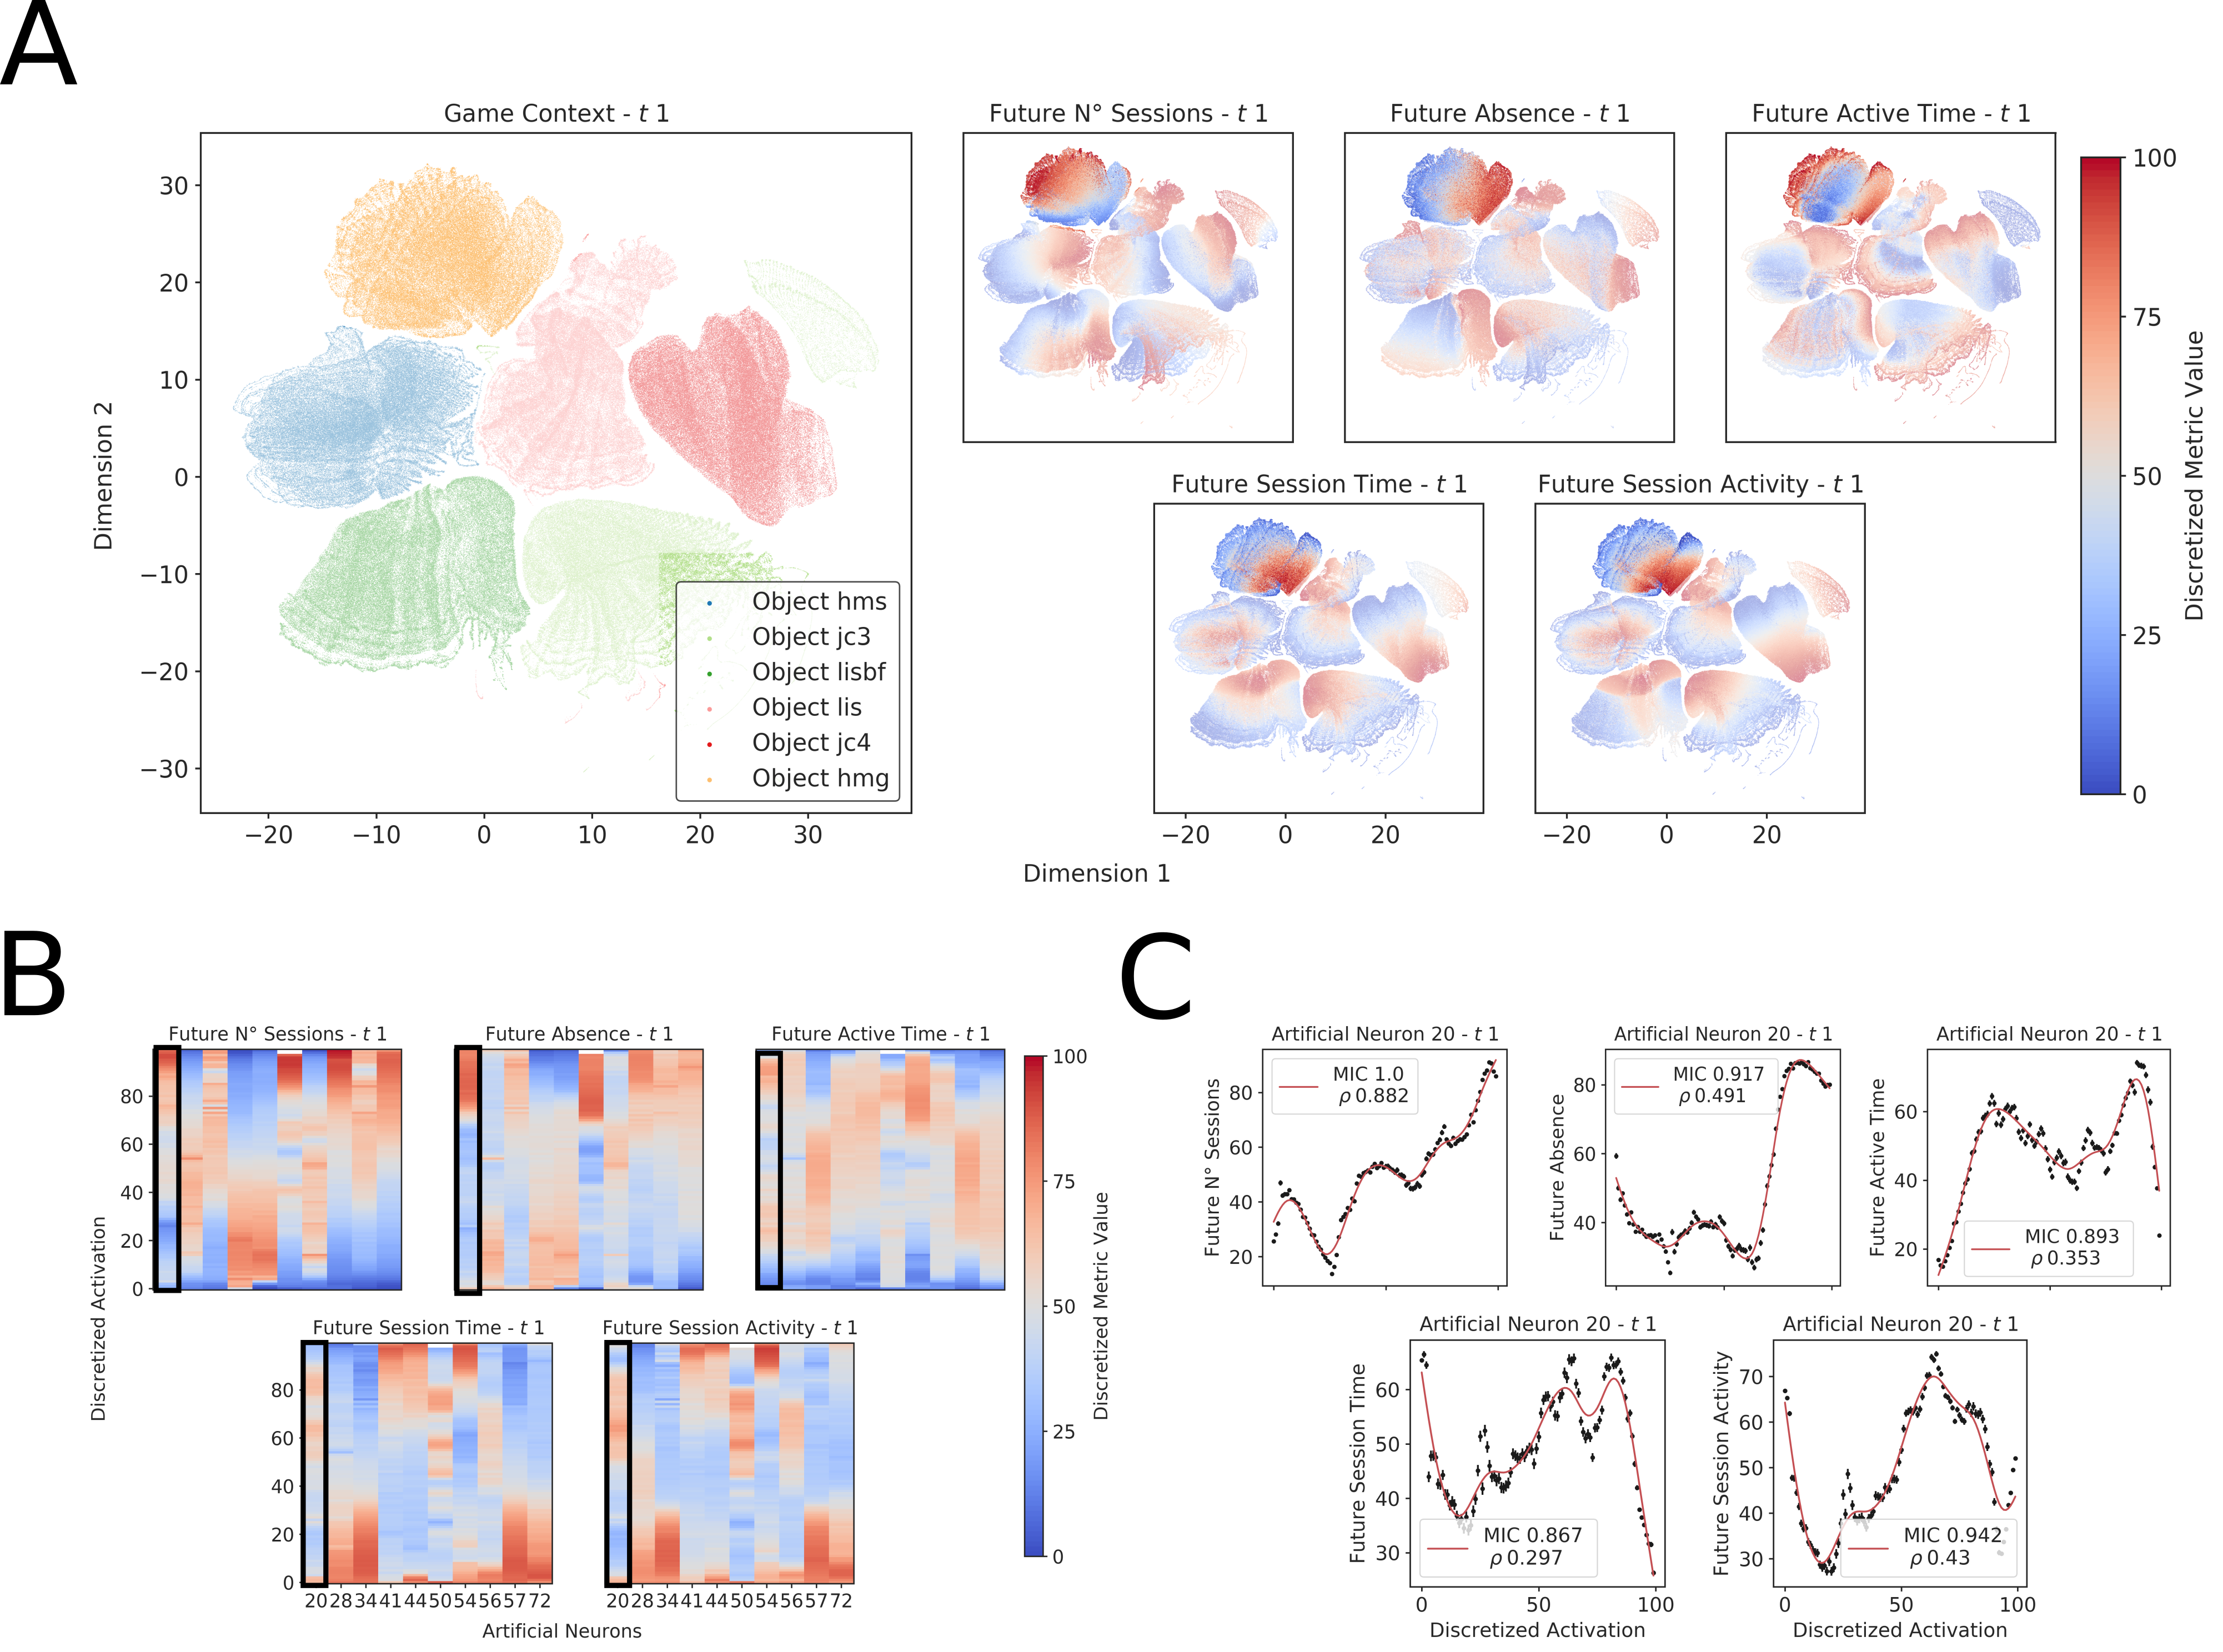
\includegraphics[width=0.9\textwidth]{images/chapter_4/static_repr_42.png}
\caption[\textbf{Lower dimensional representation of the latent state generated by the RNN architecture}]{The representation generated by the RNN model distinguishes between different game objects while maintaining an overarching organization able to capture variations in the expected intensity of future interactions that individuals will have with a specific game object. Panel A shows the two-dimensional projection, produced by UMAP, of the multi-dimensional representation inferred by the RNN at $\mathbf{t1}$ as produced by UMAP. We can read the values of the x and y axes as a coordinate system where proximity represents similarity between points in the original high-dimensional space. Each point indicates the representation inferred by the RNN model after observing one game session from a single user. The colours in the Game Context panel indicate the game object from which the representation is coming. Colours in the small panels represent the discounted sum of all future predictions for a particular target (for example, estimated Future Session Time) $\widehat{B}_{t2:T}$ which is given by $\sum_{i=0}^{t2:T} \gamma^i\widehat{B_i}$ with $\gamma=0.1$ as illustrated in equation \ref{td_v}. \textbf{Each unit  encodes the intensity of future interactions through multiple non-monotonic functions}. Panels B and C show the relationship between the activation of randomly-selected hidden units in the LSTM layer of the RNN and the model's predictions at $\mathbf{t1}$. Panel B shows the relationship between the discretized activation of 10 randomly selected units (artificial neurons) plotted along the y axis and the predictions made by the model at $t1$ (colour coded from blue to red as in the small panels in A) for the game object $hmg$. Panel C shows in more detail the relationship between discretized activation and RNN predictions for a single unit highlighted by a black box in Panel B. Here the x axis indicates the discretized activation while the y axis the mean discretized discounted sum of all future predictions produced by the model. Vertical lines are standard errors of the mean. The red curve is the line of best fit provided by a generalized additive model \cite{serven2018} while the box reports the MIC and the correlation coefficient (Spearman's $\rho$) between the artificial neuron activation and the model's predictions.}
\label{full_panel_static}
\end{figure}
The analyses in Figure \ref{full_panel_static} were performed at a single time point $t1$. When performed at subsequent time points the results appear to be qualitatively similar. For example, focusing on Future Session Time (see Appendix \ref{appendix_representation} for results connected to other targets), we see in Figure \ref{full_panel_temporal}A that the model's ability to segregate different game objects while providing an  overarching representation of the intensity of future interactions is preserved over time. This supports the hypothesis that the representation inferred by our model is dynamic in nature which is further corroborated by panel \ref{full_panel_temporal}D. There we can see how the RNN model was able to individuate a "space" with temporally consistent ”hot” and ”cold” regions between which individuals moved over time depending on the expected intensity of their future interactions. This means that given the history of interaction of a particular individual with a specific game object, our model would determine their "position" (i.e. their "internal state") in the "attributed incentive salience space". This aligns with the manifold hypothesis mentioned in sections \ref{manifold_state} and \ref{manifold_learning}: changes in the propensity to interact with a specific game object (i.e. variations in the amount of attributed incentive salience) can be expressed moving on a manifold embedded within an $h$ dimensional space, with $h$ being the dimensionality of the representation generated by our RNN model. It appears that the hidden units constituting this representation tend to be consistent over time in the type of functions they encode (see Figure \ref{full_panel_temporal}B and C). As expected, we can again observe a strong non linear association between units' activation and targets' predictions, see MIC values and lines of best fit. The decrease in MIC value observed in Figure \ref{full_panel_temporal}C for the artificial neuron 72 might indicate how certain units lose their informative power over time.
\begin{figure}[ht]
\centering
\includegraphics[width=0.8\textwidth]{images/chapter_4/dynamic_repr_42.png}
\caption[\textbf{Lower dimensional representation of the evolution of the latent states generated by the RNN architecture}]{The representation generated by the RNN model appears to maintain its discriminant properties over time. Panel A shows a two-dimensional projection of the multi-dimensional representation inferred by the RNN at $t2$, $t3$ and $t4$. The inferred representation maintains its gradient-like organization over time with an increased ability to differentiate between game objects. As in Figure \ref{full_panel_static}, x and y axes are dimensions individuated by the UMAP algorithm and can be interpreted as a coordinate system where proximity represents similarity between points. Colours in the first row indicate which game object the representation is coming from while those in the second row indicate the discounted sum of future predictions for a single target (i.e. "Future Session Time"). \textbf{The units constituting the generated representation encode for functions that are consistent over time.} Panels B and C show the relationship between units' activation and the model's predictions over time for the game object $hmg$. Different units appear to encode the same target with different non non-monotonic functions which are relatively consistent over time. Panel B illustrates the relationship between the same 10 randomly selected units specified in figure \ref{full_panel_static} and the predictions made by the model for Future Session Time at $t2$, $t3$ and $t4$. Panel C shows in more detail the relationship of the three artificial neurons, highlighted by black boxes in B, across time. Each row is a different unit while each column corresponds to a different $t$. The x axis indicates the discretized activation while the y axis the mean discretized discounted sum of all future predictions. Vertical lines are standard errors of the mean. The red curve is the line of best fit provided by a generalized additive model \cite{serven2018} while the box report the MIC and the correlation coefficient (Spearman's $\rho$) between the artificial neuron activation and the model's predictions. \textbf{The generated representation produces areas of low and high expected intensity among which individuals move over time.} Panel D shows trajectories through time produced by a version of UMAP that incorporates temporal information. Data are drawn from random subsets of individuals having low, medium and high variability in their expected amount of future behaviour. The representation inferred by the RNN model produces "hot" (i.e. the left side) and "cold" (i.e. the right side) regions, representing high and low expected Future Session Time, that are spatially consistent over time. Individuals appear to either stay in the same region or to move between regions over time. Here each line represents variations in the representation generated by the RNN model for a single user over four temporal steps. Continuity is generated by means of cubic spline interpolation for the lines and by linear interpolation for the colours. The x and y axes are the dimensions individuated by the UMAP algorithm while the z axis indicates the associated point in time. Colours indicate the discounted sum of future predictions produced by the model at a specific point in time.}
\label{full_panel_temporal}
\end{figure}

As we mentioned in section \ref{comp_framework}, both ANNs try to predict the intensity of future behaviour given the history of interactions. They do so relying on the same type of metrics, leveraging similar computational mechanisms (i.e. multitask learning and non-linearity) and producing representation according to the same underlying principle (i.e. the manifold hypothesis). Nevertheless, the fact that MLP provides poorer fit to data already suggests that whatever representation it has inferred it is likely a sub-optimal approximation of the manifold structure of incentive salience. Looking at figure \ref{predictive_panel}A, and knowing that UMAP represents differences and similarities between points through distance, we can see how the representation generated by the MLP less clearly differentiate between game objects. On the same figure, we can notice how the gradient representation for the metric Future N° Sessions Time is largely disrupted. This effect is however consistently less pronounced for other metrics (see our \href{https://htmlpreview.github.io/?https://github.com/vb690/approx_incentive_salience/blob/main/notebooks_html/embedding_analysis.html}{GitHub} for additional visualizations), in accordance to the differences we observed in predictive performance (see Figure \ref{model_comp_non_coll}). Recalling what mentioned in section \ref{comp_framework}, the latent state produced by the level of attributed incentive salience should retain at any point in time some predictive power over the intensity of all the future interactions (i.e. not just the one that follows). Figure \ref{rnn_future}B shows the representation generated by RNN and MLP at $t1$ but color coded with the discounted sum of the predictions made from $t4$ onward. We can see that, even if degraded, RNN still preserves some of the desired gradient-like organization which is instead much more disrupted for MLP. This is in accordance to what is shown by Figure \ref{full_panel_temporal}D: the RNN appears to define regions of high and low expected behavioural intensity which are consistent over time rather than constrained to the region around $t+1$.
\begin{figure}[ht]
\centering
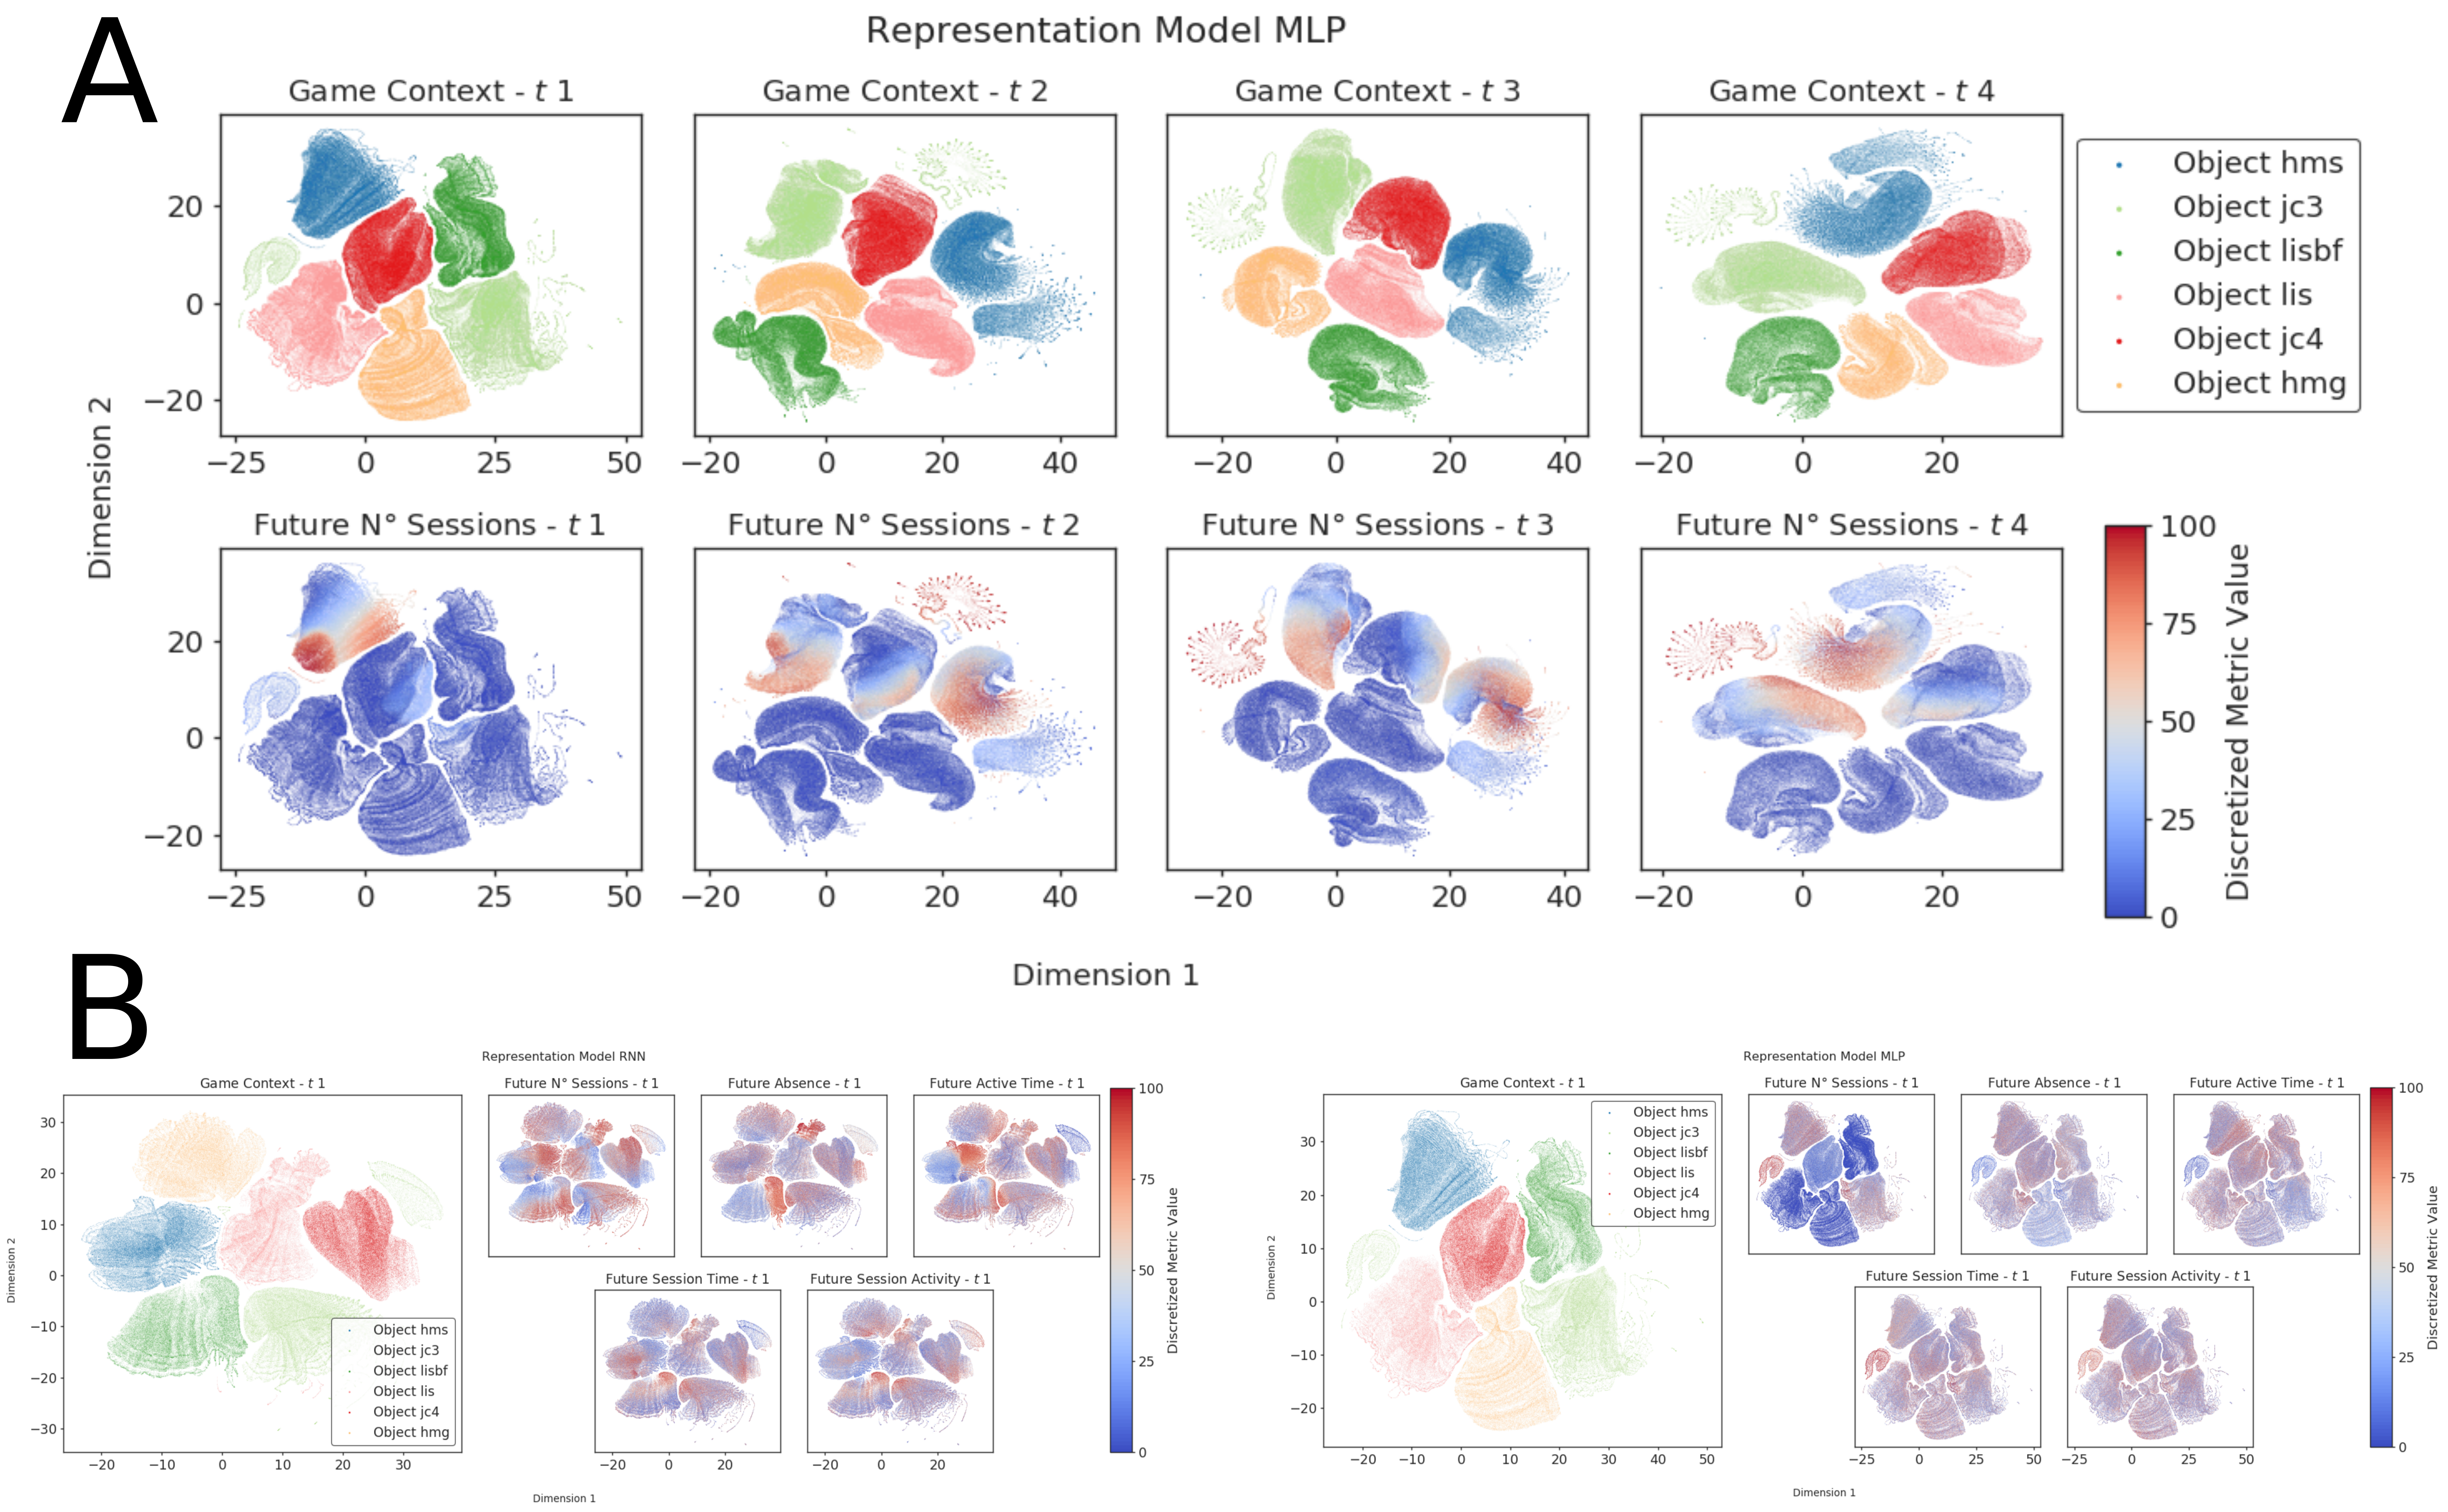
\includegraphics[width=0.9\textwidth]{images/chapter_4/RNN_MLP_repr_42.png}
\caption[\textbf{Lower dimensional representation of the latent states generated by the time-distributed MLP architecture}]{The representation generated by the MLP model is less effective at distinguishing between different game objects and different levels of expected future behaviour intensity. Panel A shows a two-dimensional projection of the multi-dimensional representation inferred by the MLP at $t1$, $t2$, $t3$ and $t4$. Differently from the RNN, the representation shows a disruption in the gradient-like organization and a reduced ability to differentiate between game objects which remain constant over time. The x and y axes are dimensions individuated by the UMAP algorithm and can be interpreted as a coordinate system where proximity represents similarity between points. Colours in the first row indicate which game object the representation is coming from while those in the second row indicate the discounted sum of future predictions for a single target (i.e. "Future N° of Sessions") \textbf{The representation generated by the MLP model is less effective at at distinguishing different levels of expected behaviour intensity for states that are further away in the future.} Panel B shows a two-dimensional projection of the multi-dimensional representation inferred by the RNN (left) and MLP(right) at $t1$ but colour coded with the discounted sum of future predictions from $t4$ onward. The representation generated by the RNN is able to maintain a gradient-like organization even from states that are further away in the future while this capacity is almost entirely lost for the MLP. The colours in the Game Context panel indicate the game object from which the representation is coming. Colours in the small panels represent the discounted sum of all future predictions for a particular target computed from $t4$ onward instead that from $t1$. The x and y axes are the dimensions individuated by the UMAP algorithm.}
\label{predictive_panel}
\end{figure}

\subsection{Model Dynamic Prediction with Covariates}
\lorem

\section{Partition Analysis}
\label{partition_analysese}
We conducted a partition analysis to individuate behavioural profiles associated with the representation generated by our model. As specified in section \ref{manifold_learning} the representation extracted by the encoder at time $t$ can be interpreted as a set of coordinates on the manifold generated by the RNN model after observing $t$ game sessions. Partitioning this representation allows us to identify areas of the manifold that hold information about the history of interactions between an individual and a video game object. These areas may represent variations in the levels of attributed incentive salience and therefore be associated with distinct patterns of behaviour. To partition the data, we used an unsupervised approach applying Mini-Batch K-Means \cite{sculley2010web}, a variation of K-Means, to the representation extracted by the encoder. Given a dataset, the algorithm attempts to divide it by iteratively moving $k$ centroids so as to reduce variance within each partition. The choice of Mini-Batch K-Means was dictated by the fact that it is one of the few distance-based algorithms that scales to very large datasets. To select the optimal $k$ value, we first fitted the algorithm with a varying number of centroids (i.e. 2 to 10) and computed the associated "inertia" (here, a measure of within cluster variance). Since inertia tends to zero as $k$ approaches the number of points in the dataset, we defined the optimal number of partitions as the value of $k$ at which the inertia reached its "elbow" or maximum curvature \cite{satopaa2011finding}. This allows to individuate at which number of partitions there are diminishing returns in terms of within cluster variance reduction. Every instance of Mini-Batch K-Means was initialized 3000 times at random and ran for a maximum of 3000 epochs. The input data were re-scaled to have zero mean and unit-variance and passed to the algorithm in random batches of size $(512 \times h)$. The associated behavioural profiles were found by applying this methodology separately to each game object and retrieving for each partition the mean of all the behavioural metrics over time. The Mini-Batch K-Means implementation used for this analysis was provided by the python library scikit-learn \cite{scikit-learn}. \\
\\
All the analyses were conducted using Python programming language version 3.6.2 \cite{10.5555/1593511}.

\subsection{Model Dynamic Prediction}
\lorem

\subsection{Model Dynamic Prediction with Covariates}
\lorem

\subsection{Discussion}
As mentioned in section  \ref{incentive_salience}, incentive salience attribution produces latent representations of objects which, when imbued with value, make future interactions with those objects more likely and intense \cite{berridge1998role,berridge2004motivation}. The representation generated by our model showed similar functional properties in their global-local organization. At the global level, different game-objects were organized in distinct and coherent regions (see Figure \ref{full_panel_static}A) showing how the model attempted to operate on a meta-level by partitioning a global representation in several object-specific ones. This finding aligns with what highlighted in various work on neural manifold where the responses related to qualitatively different stimuli tends to show a cluster-like organization when reduced to a lower dimensional space \cite{stopfer2003intensity, gallego2017neural, ganmor2015thesaurus}. At the local level, each object-specific representation showed an internal gradient-like organization distinguishing individuals based on the estimated intensity of their future interactions with that specific object. This was true for each of the considered behavioural targets (see Figure \ref{full_panel_static}A) showing how the model attempted to provide an holistic description of the intensity of future interactions. The presence of this type of gradient-like organization emerged in a work by Nieh et al. \cite{nieh2021geometry} when analyzing neural responses during an evidence accumulation task in virtual reality. When reducing the neural activity to a 3 dimensional space, the resulting manifold presented a clear gradient able to code simultaneously for position and levels of accumulated evidence \cite{nieh2021geometry}. A similar finding was present in the work by Stopfner et al. \cite{stopfer2003intensity} where the manifold structure extracted from the activity of olfactory neurons was able to represent qualitative and quantitative differences between odours through a global-local organization similar to that showed in section \ref{repr_results}. The dynamic nature of the representation generated by our approach also nicely fits with that of attributed incentive salience \cite{toates1994comparing,robinson1993neural,zhang2009neural,tindell2009dynamic,berridge2012prediction}. In particular, the fact that the aforementioned global-local organization is maintained over time (see Figure \ref{full_panel_temporal}A) corroborate the hypothesis that our model approximated state changes originated from a dynamic process. In support of this, we also observed that the representation generated by our model was spatially coherent over time: it produced distinct regions of low and high expected intensity between which individuals moved over time (see Figure\ref{full_panel_temporal}D). These results appear to match the definition of motivation and incentive salience attribution specified in section \ref{motivation}: a single overarching process able to dynamically predict the likelyhood and intensity by which individuals will interact with a varied set of objects \cite{simpson2016behavioral,toates1994comparing,berridge2004motivation,zhang2009neural}. Many other cognitive and affective functions might rely on a latent representation that is functionally similar to the one described in our work (e.g. credit assignment and optimal control \cite{wang2018prefrontal, barto2004reinforcement}, cognitive control, learning \cite{skinner1965science} or various forms of reward processing \cite{schultz1997neural, schultz2000reward}). Similarly to attributed incentive salience, these functions are all involved in generating motivated behaviour and heavily rely on reward signals, however none of them is concerned with attributing and describing the motivational saliency that an object possess. This is made evident in the works by McClure et al. \cite{mcclure2003computational} and Zhang et al. \cite{zhang2009neural} where the system involved in salience attribution is functionally separate from the one assigning credit and executing actions: the former provide a representation that informs and biases the decisions taken by the latter serving an almost exclusively qualifying role (see the role of attributed incentive salience in addiction-like conditions \cite{robinson1993neural}). Similarly, the representation generated by our model doesn't provide any insight on the decision making process underlying the observed playing behaviour but simply provide an approximate description of the "motivational pull" that a particular game object has on a particular individual at a certain point in time. The functions encoded by the hidden units constituting the representation appeared to have a series of distinctive properties, namely: redundancy, non linearity, multiplicity (single units code for multiple functions) and consistency over time. These may have played a role in providing the representation generated by our model with its distinctive characteristics. For example, as we mentioned in section \ref{manifold_state} redundancy and inter-correlation are characteristics of the signals from which the manifold representation of internal states arises \cite{seung2000manifold,gallego2017neural}. Multiplicity on the other hand, might be the factor underlying the ability of our model to produce a single unitary representation which holds predictive power over different behavioural targets. Finally, consistency over time could be the mechanisms supporting the type of temporal coherence observed in panel \ref{full_panel_temporal}D. We want to stress that these findings are to be considered exploratory in nature since they do not rely on a-priori hypotheses. A comparison between these computational properties and those underlying the attribution of incentive salience is required and would constitute a potential venue for future investigations. This supports the idea that our approach, by giving full access to its constituent parts, provides a certain degree of interpretability and offers the possibility of generating testable hypotheses. The partition analysis revealed a set of diverse profiles that largely reflect expected behavioural correlates of different levels of attributed incentive salience (i.e. high vs low intensity profiles) \cite{berridge2004motivation}. The various offsets that each partition showed might suggest different levels of predisposition towards the individual game-objects. The dynamic nature of these profiles provided a more granular characterization allowing to observe variations in the entire history of interactions and not just in the expected intensity of future ones. For example, it was possible to see how a higher likelihood of future interactions was supported both by a history of low intensity but high frequency interactions as well as by a series of high frequency and high intensity interactions (see partitions 1 and 2 in Figure\ref{partitioning}B). In this sense, these behavioural profiles can be seen as useful devices for investigating the existence of inter-individual differences in schedules of interactions with potentially rewarding objects.


\chapter{Model Application and Pipeline}
\label{chapter_appliction}
\section{Introduction}
\label{industry_needs}
As we mentioned in chapter \ref{chapter_general_intro}, the aim of this thesis has been twofold: deriving a methodology for inferring the motivational state of individuals while interacting with potentially rewarding object (a videogame in this case) and presenting how this could be used in an applied setting.

In this view, this chapter will focus on sketching the design of a system relying on our methodology for automated engagement prediction. First we will introduce a set of ethical considerations that should be taken into account when designing such system. Subsequently, we will provide an overview on why an industry player (or groups thereof) might need a process for quantifying and predicting engagement and which characteristics this process should have. Finally we will proceed at illustrating a system designed for serving this need, placing particular emphasis on how its components connect with the work presented so far.

\section{Some Ethical Consideration}
\label{ehtical_considerations}
Automated system leveraging behavioural data are now-days used extensively in both low and high stakes scenarios \cite{mehrabi2021survey}, with the potential to have a direct and concrete impact on individuals. For this reason, when designing automated data-driven applications, issues related to fairness should be taken into account. 

By fairness we entail the set of principles and considerations that in recent years are adopted in order to avoid that decisions based on a machine-learned model do not inadvertently bring harm to specific groups of people \cite{mehrabi2021survey}. A complete overview of the issue of fairness in machine learning would be beyond the scope of not just this section but the entire thesis, as it is a vast landscape \cite{mehrabi2021survey} hard to navigate due to its many levels of complexity \cite{corbett2018measure}.  We will therefore focus on two major aspects related to the work presented in this chapter. 

The first aspect concerns biases present in the data on which a machine learning algorithm is fitted. These might be induced by an over or under representation of certain strata of the population that an automated system will ultimately need to serve \cite{mehrabi2021survey}. Given how a large part of machine learning algorithms are fitted to the data (e.g., maximum likelyhood) the risk is that the prediction produced by the algorithm will revert to the mean or in the worst case, will result to be biased with respect to the true characteristics of the population \cite{corbett2018measure, mehrabi2021survey}. Despite the harm that these biases might cause in the context of engagement prediction is not as pronounced as in other areas (e.g., credit, criminal or medical risk assessment), they can still have unexpected repercussion on an individual. 

To this connects the second aspect of fairness that we want to highlight, namely the risk of inadvertently cause harm to individuals which are either temporarily or structurally subject to some form of vulnerability. This might happen as a consequence of automated decision making based on what we call "unconstrained model predictions"


for example if we imagine a system aimed at target high spender users in a game based on gatcha or loot-box mechanics, an unconstrained prediction might inadvertently target individual with a predisposition to or an history of problematic gambling behaviour.

\section{Engagement Quantification and Prediction for the Videogames Industry}
\label{industry_needs}
As we mentioned before despite the industry might be interested in the development of research projects the the focus of this project is less on the advancement of the research field on more focused on the solution of practical problems. 

In this view how does engagement connects with practical problems that the industry has? Very often (if not always) the success of a videogame title is strictly connected with either its ability to retain users or with the experience that users had with the product. The first is pivotal in scenarios where game is treated as a service sold to an audience (similarly to the function of streaming services) while the second is more relevant in scenarios where games are considered digital goods. 

In this context, engagement can be viewed as a measure of how a particular game was, is or will be able to retain users: if an individual is engaged with a particular service it is likely that will keep take advantage of it similarly if an individual had a particular good experience and gladly engaged with a particular digital good it is is more likely that will either suggest it to other users, buy similar products or buy product from the same seller.  

In this view being able to estimate the current propensity of a user towards a specific game translates (in a more or less direct way) to the capacity of assessing if a game is likely to be a success of public and revenue. For this reason it is often the case that videogame publishers and studios try to leverage the information they have available through telemetry system for taking the stock of how a particular game is performing. This is the classical example of analytical reports summarizing various type of game related Key Performance Indicators. 

\section{Multi-context Automated Engagement Prediction and Quantification}
\label{industry_needs}

\section{Data Generation}
\lorem
\subsection{Users}
\lorem
\subsection{Game Contexts}
\lorem

\section{Model Owner}
\lorem
\subsection{Data Storage}
\lorem
\subsection{Model Generation}
\lorem
\paragraph*{Data Generators} \lorem
\paragraph*{Model Configurations} \lorem
\paragraph*{Model Tuning} \lorem
\paragraph*{Model Training} \lorem
\paragraph*{Model Validation} \lorem
\paragraph*{Model Serving} \lorem

\section{Model Consumer}
\lorem
\subsection{Representation Sharing}
\lorem
\subsection{Profile Generation}
\lorem
\subsection{Live Predictions}
\lorem
\subsection{Automated Reporting}
\lorem

\begin{figure}[ht]
\centering
\includegraphics[width=0.7\textwidth]{images/chapter_5/pipeline_diagram.png}
\caption[\textbf{Model Deployment Pipeline}]{The figure represents a simplified system diagram for a potential application of the improved RNN architecture. Solid lines represent low-level components in the system while dashed lines indicate high-level entities. Directional arrows represent the flow of operations inside the system.}
\label{pipeline}
\end{figure}

\chapter{General Discussion}
\label{chapter_general_discussion}
\section{Contributions}

We will now proceed at summarizing the contribution of each chapter in the thesis along with a reflection on its limitations and the potential future research directions that could be taken in order to mitigate them.

\subsection{Chapter 1 - Connecting Motivation and Engagement}
\label{discussion_chapter_one}
In chapter \ref{chapter_lit_review} we focused on providing an overview of the psychological process of motivation highlighting its connection with the construct of engagement.

Relying on the framework proposed by Berridge et al. \cite{berridge1998role} we illustrated how motivation can be seen as process generating latent representations of objects informative of their capacity to produce rewarding experiences. We also illustrated how these representations act as modulatory mechanisms promoting or discouraging future interactions with said objects \cite{berridge2004motivation}.

Through a brief overview of the literature we showed how engagement with digital games can often be described in terms of the cognitive, emotional and behavioural manifestations resulting from the interactions that individuals have with particular game-object \cite{boyle2012engagement, jennett2008measuring, przybylski2010motivational}. These manifestations seem to arise from the interaction between the internal state of the individuals and the structural characteristics of the game \cite{lucas2004sex,o2008user,jennett2008measuring,boyle2012engagement,connolly2012systematic,csikszentmihalyi2014toward}. Moreover, the environment surrounding the individual appears to also have a role in this acting as a modulatory factor \cite{o2008user, bialas2014cultural, vihanga2019weekly, zendle2022transnational}.

Despite various attempts in the literature have been made for connecting these two processes \cite{przybylski2010motivational, nacke2011brainhex, deterding2022mastering}, a clear mechanistic description of this relationship was not always present. In this view, one major contribution of this chapter has been to outline a unifying theoretical framework for understanding the connection between neuroscientific theories of motivation and  two entities. We proposed to see motivation as a latent process arising from the interaction between individuals and (potentially rewarding) objects (i.e., videogames) and to consider engagement as its (noisy) manifestation in the observed behavioural space. 

Relying on this idea, we also highlighted the similarity between data-driven methodology for engagement prediction in a videogame context and latent variable models used in the behavioural neuroscience literature. In particular we showed that if we consider the functional goals a certain motivation-related processes (e.g., incentive salience attribution \cite{berridge2004motivation}) it is possible to understand engagement prediction models as supervise variations of certain latent variables models \cite{luxem2020identifying, mccullough2021unsupervised}.

\subsection{Chapter 2 - From Computational To Supervised Learning Models}
\label{discussion_chapter_two}
In chapter \ref{chapter_theory_modelling} we attempted to translate a computational model used for describing a specific type motivation-related latent process (i.e. attributed incentive salience) into a methodology for approximating such process within a supervised learning context.

The major contribution of this chapter has been to lay out a theoretical framework justifying the use of ANN for generating latent representations that would approximate the construct of attributed incentive salience. In particular, based on existing computational models \cite{mcclure2003computational, zhang2009neural} we illustrated why ANN, and their recurrent variant in particular, would be best suited for the task. We also proposed a series of architectural constrained designed  to encourage an ANN to generate latent representations compliant with the functional characteristics of attributed incentive salience. These were

\begin{enumerate}
    \item The use of a global model architecture for obtaining a single representation able to encompass multiple objects.
    \item The use of multi-task learning in order to force such representation to be a good descriptor of observed behaviour.
    \item The use of GAM-like mechanisms in order to include covariates of interest in the model while maintaining separability and interpretability of the inferred representations.
\end{enumerate}

\subsection{Chapter 3 - Designing, Implementing and Testing the Models }
\label{discussion_chapter_three}
In chapter \ref{chapter_implementation_testing} we proceeded at designing, implementing and testing the ANN architecture presented in chapter \ref{chapter_theory_modelling}.

The contribution of this chapter has been to validate some of the assumptions that were proposed in chapter \ref{chapter_theory_modelling}. We were able to confirm the important role of recurrency and non linearity in generating latent representations with good predictive power. 

\subsection{Chapter 4 - Validating the Properties of the Representations}
\label{discussion_chapter_four}
In comparison to other works focusing on the identification of latent states (or their manifold representation) from behavioural data \cite{calhoun2019unsupervised, luxem2020identifying, pereira2020quantifying, shi2021learning, mccullough2021unsupervised}, the present methodology offers a series of advantages. It does not require the Markov assumption, it generates continuous rather than discrete state space (hence the number of hidden states doesn't need to be specified) and it relies on a more easily scalable class of algorithms. Moreover, in contrast with a general tendency of utilising completely unsupervised techniques for capturing the manifold structure underlying behavioural data \cite{calhoun2019unsupervised, luxem2020identifying, pereira2020quantifying, shi2021learning, mccullough2021unsupervised}, our methodology attempts to extract representations which obey to specific functional constrains (see section \ref{manifold_learning}) and can therefore be more easily interpreted within a specific theoretical framework.

\subsection{Chapter 5 - Illustrating Industrial Applications of the Models}
\label{discussion_chapter_five}

Multi context engegemnt prediction
Multi objective engagement prediction
Dynamic engagement prediction
providing unifying framework for prediction and profiling within the same model.
It generates a representation that can be analyzed (similarly to what has been done in section \ref{representation_analysis}) or provided as input to other algorithms. Indeed, the encoder mentioned in section \ref{representation_analysis} can be thought of as an automatic feature extractor. This can be used to reduce complex time series data of varying length to fixed-size vectors able to describe the propensity of an individual to interact with an object. For example, the analysis presented in section \ref{partition_analysis} showed how this process could be applied for time-series partitioning of large dataset.

The present work leveraged data coming from video games but the adopted approach could easily be applied to other contexts. They only key requirement is the access to behavioural quantifiers describing the amount and intensity of interactions that an individual has with a particular object, service or task. This means that natural areas of application for our approach are those relying on the remote acquisition of behavioural data (e.g. web services or online experiments) but also situations in which large volumes of experimental data are available (e.g. large multi-center studies). 

\section{Conclusion}
In the present work we outlined a methodology for approximating motivation-related latent states in situations where large volumes of behavioural data are available but not direct contact with the individuals that generated them is possible. While doing so we tried to respect computational and theoretical constrains provided by previous works in the field of behavioural and affective neuroscience. 

Indeed we showed that it possible to embed theory-driven knowledge in data-driven approaches, allowing to more easily interpret and test hypotheses on the representation they produce. In comparison to other works focusing on the identification of latent states (or their manifold representation) from behavioural data \citep{calhoun2019unsupervised, luxem2020identifying, pereira2020quantifying, shi2021learning, mccullough2021unsupervised}, our methodology offered a series of advantages. It did not require the Markov assumption, it generated continuous rather than discrete state space and it relied on a more easily scalable class of algorithms. 

Moreover, in contrast with a general tendency of utilising completely unsupervised techniques for capturing the manifold structure underlying behavioural data \citep{calhoun2019unsupervised, luxem2020identifying, pereira2020quantifying, shi2021learning, mccullough2021unsupervised}, our methodology attempted to extract representations which obeyed to specific functional constrains therefore resulted to be more easily interpreted within a specific theoretical framework. In this view, despite our work never aimed at modelling specific cognitive or brain functions, we showed how it is possible to leverage computation model of such functions for designing data-driven methodologies for their inference. This appeared to be important in two fundamental ways. First, it allowed to construct data-driven solutions in a more principled way, rooting their functional form in the nature of the problem they were trying to solve. Second, it made it easier to a-priori specify theory-informed hypotheses and compare them against the behaviour of an otherwise black-box approach.

By connecting this methodology to the construct of engagement we showed how it could be leveraged within an industrial setting as a component of a system designed to perfrom cross-games automated engagement prediction and quantification.

\section{Limitations and Future Directions}
\label{discussion_limitations}
The work we just presented is not exempt from limitations. 

The 

Despite our findings seem to suggest a similarity between the functional characteristics of the representation inferred by our approach and the construct of attributed incentive salience these are the result of mostly qualitative, descriptive or exploratory analyses. 
Since our approach is attempting to solve an inverse problem, the issue of uniqueness arises. Many different latent states might have produced the behavioural patterns that our model observed and there is no guarantee of a strict one-to-one mapping between the representation generated by our model and attributed incentive salience.  More effort should be posed in future research for obtaining a clear formulation of the computations carried out by our architectures. Alternatively, an extensive work of validation could be carried out by comparing the representations generated by our architectures with those generated from data gathered through laboratory or simulation experiments. 

The behavioural profiles individuated in section \ref{partition_analysese} by our partition analyses generally reflect those predicted by theories of reward-driven motivation \citep{thorndike1927law,skinner1965science,berridge2004motivation} but they also show some unexpected and potentially contradictory results. Given the observational setting of our work and the unsupervised approach we adopted, the explanations provided in section \ref{partition_analysese} should be taken with caution and be seen as a method for generating testable hypotheses that should constitute the starting point for future investigations. Indeed, clarifying the the nature of some of the observed discrepancies may require experimental work in more controlled settings. Lastly, despite our approach appeared to deal gracefully with objects having different structural characteristics, these were limited to the domain of video games. In order to verify the generalizability of our approach, future work should include data generated from a variety of contexts (e.g. web services, online and laboratory-based experiments).  



\bibliographystyle{unsrt}
\bibliography{bibliography}

\end{document}

%%%%%%%%%%%%%%%%%%%%%%%%%%%%%%%%%%%%%%%%%%%%%%%%%%%%%%%%%